%% Select the dissertation mode on
% See the documentation for more information about the available class options
% If you give option 'draft' or 'draft*', the draft mode is set on
\documentclass[dissertation,draft*]{aaltoseries}
\usepackage[utf8]{inputenc}
% Lipsum package generates bullshit
\usepackage{multirow, amsthm, amssymb, amsmath,natbib, algorithm, algorithmic, amsxtra, txfonts}
% Set the document languages
\usepackage[finnish,swedish,english]{babel}

\newtheorem{theorem}{Theorem}
\newtheorem{lemma}[theorem]{Lemma}
\newtheorem*{definition}{Definition}

\newcommand{\E}[1]{\mathrm{E}[ #1 ]}
\newcommand{\prob}[1]{\mathrm{P}( #1 )}

% The author of the dissertation
\author{Lauri H\"ame}
% The title of the thesis
\title{Demand-Responsive Transport: Models and Algorithms}

\begin{document}

%% The abstract of the dissertation in English
% Use this command!
\draftabstract{
Demand-responsive transport is a form of public transport between 
bus and taxi services, involving flexible routing of small or medium sized vehicles.
This dissertation presents mathematical models for demand-responsive transport and methods
that can be used to solve combinatorial problems related to vehicle routing and journey planning
in a transport network.

Public transport can be viewed as a market where demand affects supply and vice versa.
In the first part of the dissertation related to vehicle routing, 
we show how a given demand for transportation can be satisfied by using a fleet of vehicles,
assuming that the demand is known at the individual level. In the second part, by considering 
the journey planning problem faced by commuters, we study how the demand adapts to the 
supply of transport services, assuming that the supply remains unchanged for a short period of time.
In the third part we present methods
for determining the economic equilibrium, that is, the point at which the demand meets the supply,
by assuming that commuters attempt to minimize travel time and transport operators aim to maximize profit.

The mathematical models proposed in this work can be used to simulate the operations of public transport services in 
a wide range of scenarios, from paratransit services for the elderly and disabled to 
large-scale demand-responsive transport services designed to compete with private car traffic. Such calculations can 
provide valuable information to public authorities and planners of transportation services,
regarding, for example, regulation and investments.
In addition to public transport, potential applications of the proposed methods for solving vehicle routing and journey planning problems
include freight transportation, courier and food delivery services, military logistics and air traffic.
}
% Let's add another one in Finnish
\draftabstract[finnish]{Kysynt\"aohjautuvalla joukkoliikenteell\"a tarkoitetaan 
bussi- ja taksipalvelujen v\"alimuotoa, joka perustuu pienten tai keskisuurten ajoneuvojen joustavaan reititykseen.
T\"ass\"a v\"aitöskirjassa esitet\"a\"an matemaattisia malleja kysynt\"aohjautuvalle joukkoliikenteelle ja menetelmi\"a
joilla voidaan ratkaista ajoneuvojen reitinlaskentaan ja matkansuunnitteluun liittyvi\"a kombinatorisia ongelmia liikenneverkossa.

Joukkoliikennett\"a voidaan tarkastella markkinana, jossa kysynt\"a vaikuttaa tarjontaan ja p\"ainvastoin.
V\"aitoskirjan ensimm\"aisessa osassa, joka k\"asittelee ajoneuvojen reitinlaskentaa, n\"aytet\"a\"an miten tunnettuun kysynt\"a\"an voidaan 
vastata k\"aytt\"am\"all\"a tietty\"a ajoneuvokantaa, kun oletetaan kysynt\"a tunnetuksi yksil\"otasolla. 
Toisessa osassa tarkastellaan matkustajien matkansuunnittelua joukkoliikenneverkossa eli sit\"a miten kysynt\"a
mukautuu liikennepalvelujen tarjonnan mukaan, kun oletetaan tarjonta muuttumattomaksi lyhyell\"a aikav\"alill\"a.
Kolmannessa osassa esitet\"a\"an menetelmi\"a
taloudellisen tasapainopisteen, eli kysynn\"an ja tarjonnan kohtaamispisteen, m\"a\"aritt\"amiseksi,
kun oletetaan ett\"a matkustajat pyrkiv\"at minimoimaan matka-aikaa ja liikennepalvelujen 
tarjoajat pyrkiv\"at maksimoimaan taloudellista voittoa.

T\"ass\"a työss\"a esiteltyjen mallien avulla voidaan simuloida useita erityyppisi\"a liikennepalveluja 
vanhuksille ja liikuntarajoitteisille suunnatuista kutsulinjoista 
henkilöautoliikenteen kanssa kilpaileviin laajamittaisiin kysynt\"aohjautuviin joukkoliikennej\"arjestelmiin. 
Mallien avulla tehdyt laskelmat voivat tuottaa arvokasta tietoa viranomaisille ja liikennepalvelujen suunnittelijoille 
liikenteen s\"a\"annöstelyyn ja investointeihin liittyen.
Joukkoliikenteen lis\"aksi esiteltyj\"a reitinlaskenta- ja matkansuunnittelumenetelmi\"a voidaan soveltaa muun muassa 
rahti- ja lentoliikenteess\"a, l\"ahetti- ja ruoankuljetuspalveluissa sek\"a sotilaslogistiikassa.}
% And yet another one in Swedish
% \draftabstract[swedish]{Demand-responsive transport (DRT) is an advanced, user-oriented form of public transport between 
% bus and taxi, involving flexible routing of small or medium sized vehicles.
% This dissertation presents mathematical models for demand-responsive transport and algorithms
% that can be used to solve combinatorial problems related to vehicle routing and journey planning.}

%% Preface
% If you write this somewhere else than in Helsinki, use the optional location.
%\begin{preface}[Helsinki]
%\lipsum[1-4]
%\end{preface}
\maketitle

%% Table of contents of the dissertation
\tableofcontents

%% For article dissertations, remove if you write a monograph dissertation.
\listofpublications

%% Add lists of figures and tables as you usually.

%% Add list of abbreviations, list of symbols, etc., using your preferred package/method.

%% The main matter, one can obviously use \input or \include

\chapter{Introduction}
\section{Demand-responsive transport today$\ldots$}
Demand-Responsive Transport (DRT) is often referred to as a form of public transport between bus and taxi services involving 
flexible routing and scheduling of small or medium sized vehicles. 
This means that 
the vehicle routes are updated daily or in real time by incorporating information on
the demand for transportation. Usually, the customers of a DRT service are required to
request and book their trips in advance by placing trip requests including information
on the origin and destination of the trip as well as the desired pick-up or drop-off time.
The vehicle operator uses this information to provide service in a way that the passenger
needs are satisfied.


DRT systems are typically used to provide transportation in areas with low 
transportation demand, where a regular bus service might not be as efficient. 
Another common application of DRT arises in door-to-door transportation
of elderly or handicapped people (paratransit).
%Paratransit: DRT is available to the general public, whereas paratransit is available to pre-qualified user bases
%share taxis: DRT is pre-booked in advance, whereas share taxis are operated on an ad-hoc basis
%Taxicabs: DRT generally carries more people, and passengers may have less control over their journey on the principle of DRT being a shared[4] system as opposed to an exclusive vehicle for hire. Additionally, journeys may divert en-route for new bookings.[6]
DRT services are often fully or partially funded by local 
authorities, as providers of socially necessary transport. 
%A small fraction 
Most services that are provided by private companies for commercial reasons
are related to transporting passengers between airports and urban areas.
%Demand-responsive transport services are restricted to a certain operating zone.

The implementation of demand-responsive transport is strongly dependent on the target group
or the business concept of the service. In some services, the vehicle routes are built 
freely according to customer requests, whereas 
other services make use of so-called skeleton routes and schedules, that are varied as required. 
%As such, customers are given specific pick-up and drop-off points and time windows for pick-up and drop-off. 
Some DRT systems make use of terminals, at one or both ends of a route, such as an urban center or airport.
In these applications (one-to-many or many-to-one), customers may specify either the origin or destination of the 
desired trip. Some systems provide door-to-door service within a certain service area and others provide 
service between a set of specified stops. 
For example, a DRT service operating in Nurmij\"arvi (Finland) aims to improve the level and
accessibility of services in a sparsely populated area and
to reduce the costs of public transport. The service operates on
a "many-to-many" basis, that is, there are no predefined routes. 
The stop points are located at a maximum of
900 m from origins and destinations. In the case of
special users, the stop points are non-predefined (door-to-door service). 
%What is clear from the foregoing is that there is an extremely wide range of
%applications of the  

%Generally, DRT systems require passengers to request a journey by booking with a central dispatcher, who determines the 
%trip options available given the customer's location and destination.
%The vehicles used in DRT services are generally small minibuses, 
%allowing to provide a near door to door service by being able to use residential streets.

%\subsection{Strengths}
The popularity of demand-responsive transport has recently grown
mainly due to the shortcomings of conventional
bus and taxi services and new technical developments.
In addition, flexible public transport services provided by local authorities and bus operators in
partnerships with employers, stores and leisure centres are thought to help to break down social exclusion \cite{detr}.
%\subsection{Weaknesses}
However, current DRT services have often been
criticised because of their relatively high cost of provision,
their lack of flexibility in route planning and their
inability to manage high demand \cite{mageean}. 

At the present moment, a large number of demand-responsive transport services are 
in operation. Most of such services operate within relatively small neighbourhoods and 
during low-use daytime hours, when there is not enough demand for traditional 
public transport. Thus, while the current services meet their current needs,
demand-responsive transport remains a relatively small business
compared to traditional transportation services, not to speak of private cars.

What if a DRT system was implemented in large scale, in a way that service could be provided
for an entire metropolitan area?

\section{$\ldots$and tomorrow}
Several new ideas and concepts related to demand-responsive transport
services operating in urban areas have been recently presented, see for example \cite{cortes,jokinen-fists-2011}, \ref{cpooling}.
These ideas are often motivated by problems arising from the congestion of urban 
areas caused by the increasing number of private cars.
Thus, one of the main present goals of planning demand-responsive transport is seen
to be the developing of \emph{functional public transport services able to compete
with private car and taxicab traffic}.


The popularity of the private car as a means of transport is partly based on
a direct connection between the origin and destination of a trip and
a short total travel time. In order to compete with private cars, public transport 
should thus offer connections as direct and fast as possible, in which 
the walking and waiting time are minimized. 
Another major advantage of the private car is seen to be the availability
of the car at any time, even without planning beforehand. The study of large scale 
demand-responsive transport has therefore been directed towards highly dynamic services, which allow 
customers to request service not long before they are willing to depart.
In addition, a demand-responsive public transport system should be
able to offer an alternative for transportation without
the inconvenience related to conventional public transport.

%The popularity of the private car as a means of transport is based on
%a direct connection between the origin and destination of a trip and
%a short total travel time. Thus, to compete with private cars, a transportation system 
%should offer connections as direct and fast as possible, in which 
%the walking and waiting times of customers are minimized. 
%In addition, a demand-responsive transport service should be
%able to offer an alternative for transportation without
%the inconvenience related to conventional public transport.

The total travel time in public transport consists of
\emph{walking time} from origin to pick-up point, \emph{waiting time} at
the pick-up point, \emph{ride time}, that is, the time spent in the
vehicle, possible \emph{transfer time} and walking time from 
drop-off point to destination. In order %for this door-to-door travel time
to attract people with private cars, it is necessary that the waiting and 
riding times are within acceptable bounds. In addition, it can be suggested that
the service should be a near door-to-door service and the amount of
transfers between vehicles should be minimal. 

Intuitively, the idea of a large scale DRT system seems promising.
With state-of-the-art engineering, there should be no insuperable technical hindrances
in implementing such a service.

%In the following sections, the strengths and weaknesses of a large scale DRT
%system providing a high level of service are examined.

\subsection{Opportunities}
The fact that demand-responsive transport is "there for you when you want
and where you want" is thought to be a major advantage compared to conventional 
public transport. While it may not be feasible to think that DRT could provide
a level of service substantially better than that offered by taxi cabs, a system that could combine customers'
trips efficiently could be more cost-efficient than a conventional taxi organization.
This would make it possible to provide more inexpensive service without compromising
too much on the level of service experienced by customers.
%In addition, if the trips were aggregated efficiently, and the number of vehicles
%per unit area was large, the waiting times could in fact be slightly shorter compared to current
%taxi services.

Compared to private cars, demand-responsive transport is thought to have several advantages in urban areas.
%For example, the current average occupancy in private cars in the Helsinki metropolitan area is around 1.3.
For a model of a hypothetical large-scale demand-responsive public transport system for the Helsinki 
metropolitan area, simulation results published in 2005 demonstrated that "in an urban area with one 
million inhabitants, trip aggregation could reduce the health, environmental, and other detrimental 
impacts of car traffic typically by 50 - 70\%, and if implemented could attract about half of the car 
passengers, and within a broad operational range would require no public subsidies" \cite{tuomisto}. 
In addition to providing affordable transportation without the additional expenses related 
to maintenance, taxes and parking fees, 
demand-responsive transport could eliminate many other, possibly concealed, concerns related to private cars, 
including the difficulty of finding parking space and the stress related to
driving in hazardous conditions or traffic jams.

At this point, one might ask: If the large scale demand-responsive transport system is superior 
compared to the alternatives, why has it not been implemented in practice? 

\subsection{Possible issues} %Possible issues
%As previously stated, current demand-responsive transport services are often fully or partially funded by local 
%authorities. This is also true for public transport in general. Thus, 
While it is clear is that implementing a large-scale demand-responsive transport system 
would require significant investments, it is not clear 
whether there would be enough demand for such a service were it implemented. 

For example, it might not be realistic nor beneficial from the social point of view 
to think that a conventional heavy rail system was replaced by demand-responsive minibuses, 
due to the high efficiency of heavy rail.
Moreover, traditional public transport in general has many significant advantages compared to
demand-responsive transport: Taking into account the current experience from DRT services,
a major issue can be seen to be the reliability of the service. So far, estimating ride times accurately
in a service with no fixed routes has proven to be somewhat insuperable, not least because
of the human drivers, who are required to follow routes that are constantly changing, and the
differences in their driving styles. Another disadvantage of DRT arises when customers are 
required to book their trips in advance and thus commit themselves to the service or payment
at the time the trip is booked. In traditional bus services, this problem does not
exist since customers may adjust their personal schedules dynamically according to known timetables,
without pre-commitments. A commitment to a trip can be even more binding than in a taxi service:
A normal taxi can wait for some time for the customer, for example, if the customer is at home 
when the taxi arrives, but it might not be reasonable that a demand-responsive minibus with 
customers on board would wait many minutes for one customer with the expense of other customers.

While demand-responsive transport has many rewards compared to the private car as argued above,
the car has many characteristics that are hard to compensate with public services. 
Firstly, a person who has already invested in a car and thus settles yearly taxes and
maintenance costs, is often not willing to use other transportation services since it would
cost more than the marginal cost of using the car.
Secondly, the car is unbeatable in many cases when speaking of flexibility: 
It is available at any time of the day, even without planning beforehand. 
Even if a demand-responsive transport service accepted immediate requests without
a minimum pre-order time, the customer would still be committed to wait for the 
designated vehicle to arrive. Thirdly, the private car is thought to be the most convenient 
way of carrying large amounts of luggage and goods. The car is also often used for
storing equipment, which is not likely to be possible in a public service. 
%Finally, the private car is still thought to give its owner a certain status.   

Despite the above threats related to large scale 
demand-responsive transport, the concept should be studied carefully.
Even if the private car has its advantages in the current state of the world,
it may become practically useless in congested urban areas.
%In addition, environmental issues are given a lot of consideration at the present moment.
%: % in welfare states:  Some are even ready compromise on price and quality if a service proves to be "green". 

%
%
%
%%Conventional public transport, especially heavy rail, is thought to be more
%%beneficial from the social point of view.
%
%For example, demand-responsive minibuses are not likely to be able to compete with heavy rail
%systems
%
%
%The private car,
%as a means of transport, has many advantages  
%
%
%
%
%
%
%
%%Furthermore, in order to achieve efficiency and a good level of service, it 
%%is suggested that the following elements should be given special attention.

\section{Problem statement}
This work is focused on the discrete and combinatorial problems arising in the planning of
public transport in general and demand-responsive transport in particular. The main goals are (i) to develop models for a priori studying 
different forms of demand-responsive transport without having to implement them in practice and (ii) to
develop algorithms for solving combinatorial problems related to public transport.

Generally, public transport can be viewed as a market where demand affects supply and vice versa.
For a given demand, we are interested in the optimal actions for the transport operator and for a given supply, 
we study the optimal actions for customers with specific travel needs. By relaxing both demand and supply, 
we seek to determine the economic equilibrium, where the demand meets the supply.
More precisely, the three main research questions considered in this work are stated as follows: 
%First, we assume that the demand is fixed and optimize the supply. Second, for a given supply,
%More precisely, the main problems are stated as follows:

In Chapter \ref{vehiclerouting}: \emph{Vehicle routing}, the demand for transportation is assumed to be known at the individual level. 
Using a fleet of vehicles, what is the best way to satisfy the demand? 

In Chapter \ref{journeyplanning}: \emph{Journey planning}, the schedules and routes of transport services are assumed to be known during a specific time horizon.
Using the scheduled transport services, what is the best way for a commuter to travel from a given origin to a given destination?

In Chapter \ref{economicmodels}: \emph{Economic models}, we define the demand model by assuming that customers seek trips with
small travel times and the supply model by assuming that transport service providers aim to maximize profit. Given these models,
at which point does the demand for transportation meet the supply and how do regulation policies affect the economic equilibrium?

% \subsection{Vehicle routing}
% 
% 
% In order to provide efficient stop-to-stop service, %by vehicle mileage and trip duration, 
% it is required that the pick-up and drop-off points of customers are chosen in a way that 
% the vehicle mileage and the excess ride time reflected to customers on board is minimized while 
% the walking distance remains within reasonable limits.
% 
% \subsection{Journey planning}
% A demand-responsive transport service should be compatible with other transportation
% modes. In conventional dial-a-ride services, trip bookings are made by calling the service provider, but
% a modern service should certainly be automated and enable on-line trip booking in order
% to attract a large population. This requires a route planner that is capable of 
% communicating with conventional public transport as well as DRT.
%    
% \subsection{Economic models}


% The remainder of this document is organized as follows. In chapter \ref{potential},
% the potential for passenger pooling and trip combining is evaluated by means of
% a simplified simulation model. In chapter \ref{irdarp}, the problem of dispathcing
% vehicles in a dynamic DRT service is formalized and a solution approach is described.
% Chapter \ref{simutools} introduces a generalized simulation model designed for large scale DRT and
% a collection of simulation results for an unconstrained immediate-request service.
% An adjustable single vehicle routing algorithm, an important subroutine in the proposed 
% solution, designed for constrained problems arising in real-life situations, 
% is described in chapter \ref{eadarp}.


%% Examples of article references, remove these from your manuscript!
% Uncomment them, if you want to see the results of these commands in this example document

 % Refer to the Journal paper 1 of this example document
%\citepub{j1} \& \cpub{j1} \& \cp{j1} \& \pageref{j1} \& \ref{j1}

% Refer to the Conference paper of this example document
%\citepub[p.~2]{c1} \& \cpub[Sec.~ 1]{c1} \&  \cp[pp.~1--2]{c1} \& \pageref{c1} \& \ref{c1} 

\chapter{Vehicle Routing}
\label{vehiclerouting}
A vast majority of theoretical studies related to demand-responsive transport are formalized as combinatorial
optimization problems involving the construction of vehicle routes with respect to
a set of customers, whose pick-up and drop-off points are known a priori \cite{toth03}.
This problem is often referred to as the \emph{dial-a-ride problem}.
A demand-responsive transport service operating in real time induces the following specific challenges: 
In order to be able to compete with private cars, service
should be available within a short period of time from the trip request.
This calls for routing algorithms capable of adapting to high-demand situations, since the modifications 
in vehicle routes have to be executed in real-time.
In order to ensure a sufficient level of service, the customers' waiting and ride times 
should be relatively limited. Thus, the vehicle dispatching algorithms should be designed
in a way that the constrained nature of the problem is taken into account.

In Section \ref{singlevehicle}, we study the \emph{single-vehicle dial-a-ride problem} which involves the construction
of a single vehicle route serving a set of customers. This problem is motivated by the
fact that solutions to the single-vehicle problem can be used as subroutines in environments with 
multiple vehicles \cite{psaraftis01,psaraftis02}. The extension from the single-vehicle problem to the multi-vehicle
case is dicussed in Section \ref{multivehicle}.

\section{Single-vehicle dial-a-ride problem}
\label{singlevehicle}
Different types of dial-a-ride services give rise to
different types of mechanisms for controlling vehicle operations. 
For example, if a dial-a-ride service requires customers to request 
service during the previous day, the nature of vehicle
dispatching will certainly differ from a service in which
customers may request immediate service.
This Section focuses on %, a specific version of the dial-a-ride problem (DARP) is examined, namely, 
the \emph{single-vehicle DARP with time windows}, in which the goal is to determine the optimal
route for a single vehicle serving a certain set of customers.

The consideration of time windows means that the vehicle route is 
restricted by time limits for pick-up and delivery of each customer.
Narrow time windows emerge in transport services, in which each customer
is given an estimate or guarantee regarding the pick-up and delivery times in the 
form of time windows. These time windows are examined as hard limits to be met by the vehicle.
Time windows have been incorporated in many early and recent studies of the DARP, see for example 
\cite{psaraftis02, jaw, madsen, toth02,cordeau02,diana, wong, cordeau01, berbegliafeas}.
In these studies it is noted that in dynamic settings, time windows eliminate the possibility of indefinite
deferment of customers and strict time limits help provide reliable service.
Maximum ride time constraints that limit the time spent by passengers in the vehicle
between their pick-up and their delivery \cite{hunsaker}, 
are considered as well.

In \cite{psaraftis01}, the objective function is defined as a
generalization of the objective function of the Traveling Salesman Problem (TSP), 
in which a weighted combination
of the time needed to serve all customers and of the total degree of dissatisfaction
they experience until their arrival to the destination of the trip is minimized. The dissatisfaction of
customers is assumed to be a linear function of the time each customer waits to be picked up and the 
time each customer spends riding in the vehicle until his/her delivery.
In \cite{psaraftis02}, the approach is extended to handle time windows on departure and arrival times,
but only the route duration is minimized. 

In \ref{jeadarp}, both aspects of the problem (general objective function and time windows)
are considered. The main contribution is a solution method designed in a way that (i) it is capable of
handling practically any objective function suitable for dynamic routing and (ii) the computational
effort of the algorithm can be controlled smoothly: If the problem size is reasonable, 
the algorithm produces optimal solutions efficiently and as the problem size is increased,
the search space may be narrowed in order to achieve locally optimal solutions.

Publications \cp{jhitsdarpts} and \cp{jrbrorl} discuss a single-vehicle algorithm based on hyperlink-induced topic search \cite{kleinberg} 
for maximizing the number of customers in a single vehicle route. The method is seen to
be useful in determining the feasibility of multi-vehicle instances. 

\subsection{Literature review}
In the following paragraphs, a short review on the studies related to the single vehicle dial-a-ride problem is
presented, based on \cite{cordeau03, cordeau05, cordeau07} and \cite{berbeglia}, to which the reader is referred 
for more exhaustive summaries. 

The first exact approach to the solution 
of the dynamic dial-a-ride problem was presented by \cite{psaraftis01}. 
In this work the single-vehicle, "immediate-request" case is studied, in which a set of customers should be served as soon
as possible. In this first model no time windows are specified by the customers, but the
vehicle operator incorporates \emph{maximum position shift} constraints limiting the difference between
the position of a request in the chronological calling list and its position in the vehicle route. 
The objective is to minimize a weighted combination of the time needed to serve all customers 
and customer dissatisfaction.
The complexity of this algorithm is $\mathcal{O} (n^2 3^n)$ and only small instances
can thus be solved. However, the computational effort is decreased as more strict constraints
are imposed. 

The algorithm is first constructed for the static case of the problem and then 
extended to solve the dynamic case, in which 
new requests occur during the execution of the route but no information on future requests is available.
In this version of the problem, the use of maximum position shift constraints is essential, in order 
to prevent a request from being indefinitely deferred. 
In a later study \cite{psaraftis02},
the approach is extended to handle time windows on departure and arrival times.
In this extension, only the route duration is considered in the objective
function. 

In \cite{sexton02, sexton03}, a heuristic approach to the single vehicle DARP
with one-sided time windows was introduced. 
In this problem formulation, the objective function is defined as a function of (i) the difference between the actual
travel time and the direct travel time of a user and (ii) the difference
between desired drop-off time and actual drop-off time. The algorithm was
tested on real-life problems involving 7 to 20 customers. %data sets where the number of customers varies between 7 and 20.

In \cite{desrosiers01}, an exact dynamic programming algorithm for the single vehicle DARP, formulated as an integer program, 
was presented. The formulation includes time windows as well as vehicle capacity 
and precedence constraints. Optimal solutions with respect to total route length were obtained for $n=40$.

In \cite{bianco}, exact and heuristic procedures 
for the traveling salesman problem with precedence constraints are introduced, based on
a bounding procedure. Computational results of the algorithm are given for a number
of randomly generated test problems, including the dial-a-ride problem with the classical
TSP objective function.

Psaraftis noted that \emph{although single-vehicle Dial-A-Ride systems do not exist in 
practice, single-vehicle Dial-A-Ride algorithms can be used as subroutines in
large scale multivehicle Dial-A-Ride environments. It is mainly for this reason
that one's ability to solve the single-vehicle DARP is considered important.}

\subsection{Problem formulation}
\label{staticnarrow}
Let there be $N$ customers, each of which have been assigned a number $i$ between 1 and $N$.
For each customer $i \in \{1,\ldots,N\}$, let $u_i$ be the pick-up point and $u_{N+i}$ be the delivery point,
$[E_i,L_i]$ be the pick-up time window and $[E_{N+i},L_{N+i}]$ be the delivery time window. 
In addition to the fixed time windows $[E_i,L_i]$ and $[E_{N+i},L_{N+i}]$, to each 
customer is associated a specific maximum ride time constraint $T_i^{\max}$. 
Let $q_i$ be the load (number of passengers) associated to customer $i$. 
Let $A$ be the starting point of the vehicle (location of the vehicle at $t=0$).
It is assumed that the time to go from any one of the pick-up and delivery points 
$u_i$, where $i \in \{1, \ldots, 2N\}$, directly to another point $u_{j}$ is a 
known and fixed quantity $t(i,j)$.
The above parameters are illustrated in Figure \ref{timeline01}.
\begin{figure}[ht]
\begin{center}
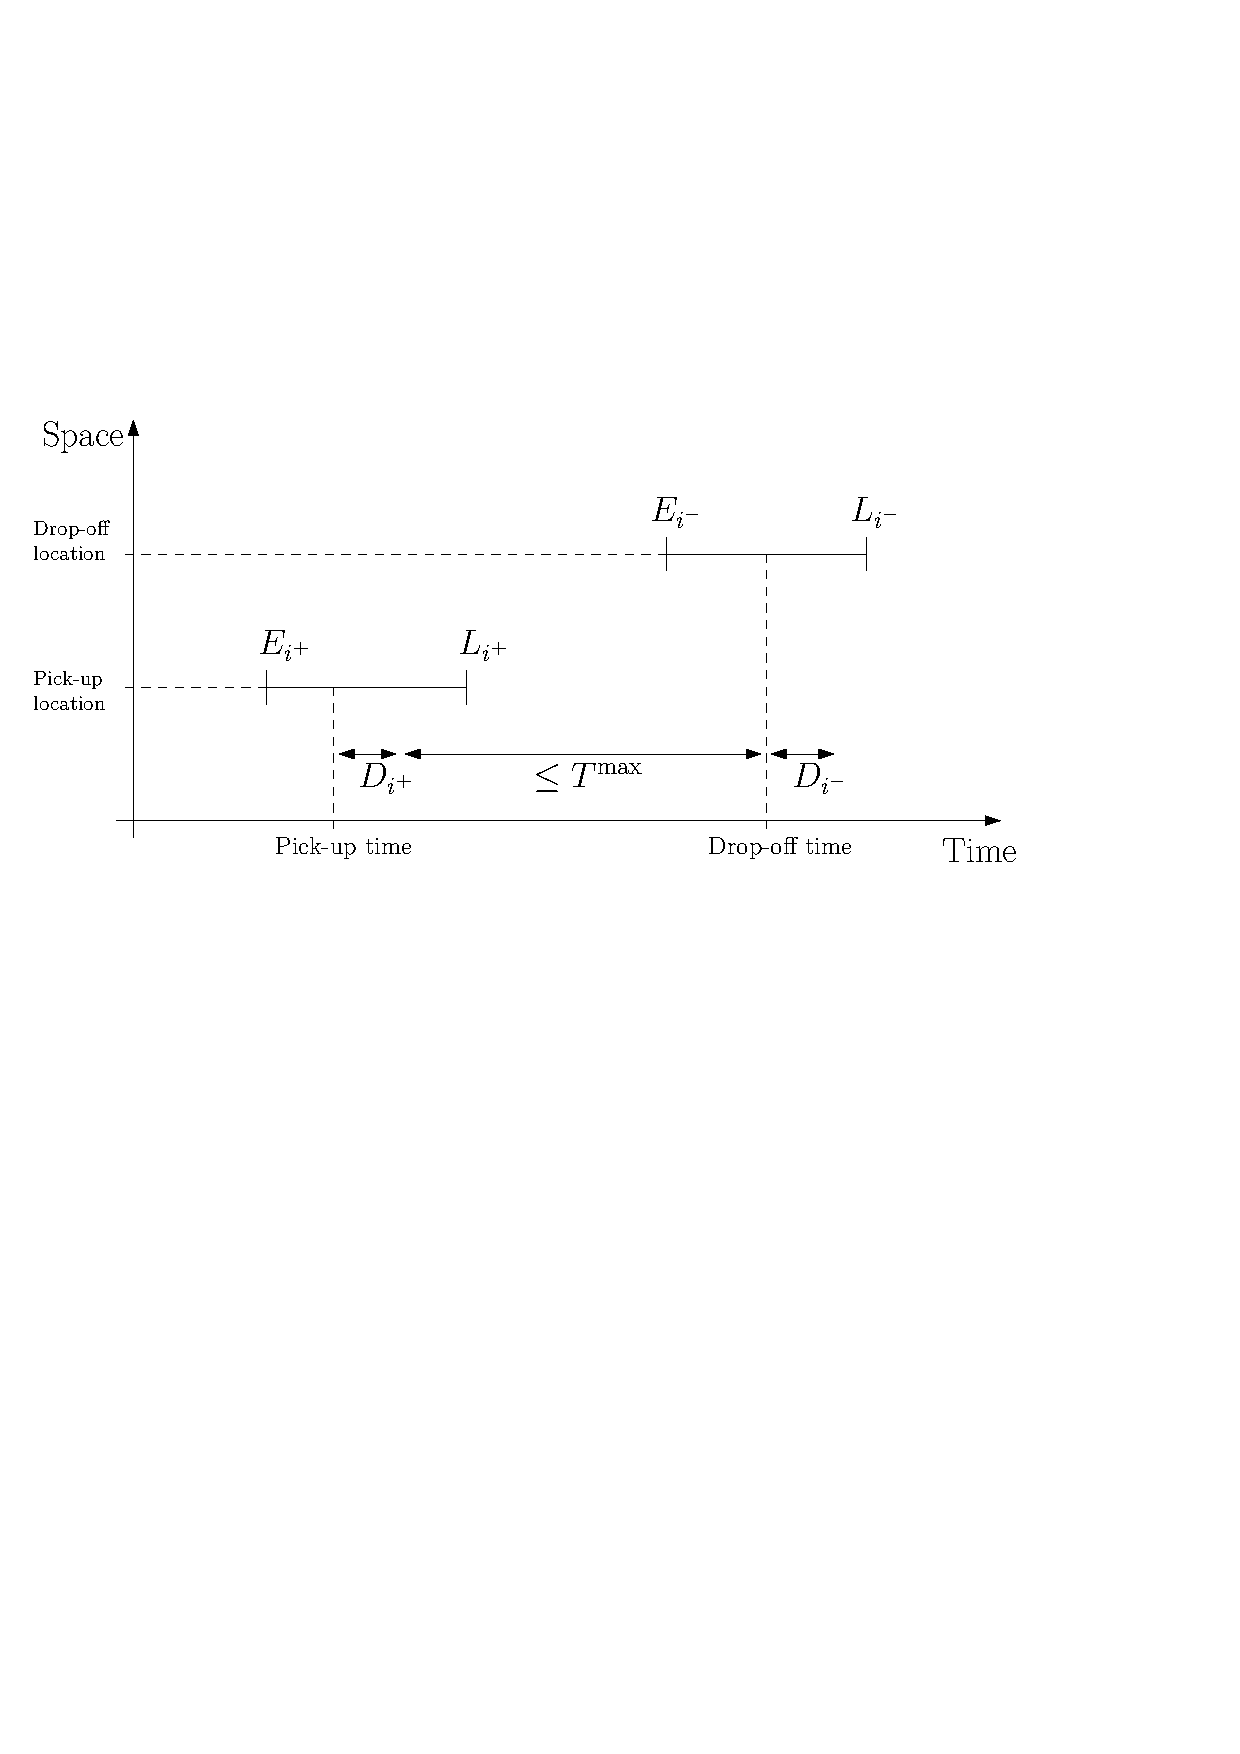
\includegraphics[width=0.9 \columnwidth]{timeline01}
\caption{Time pick-up and drop-off time windows. The pick-up point of
customer $i$ is denoted by $i^{\uparrow}$ and the drop-off point is denoted by $i^{\downarrow}$.
The customer should be picked up at $i^{\uparrow}$ within the time window $[E_{i^{\uparrow}},L_{i^{\uparrow}}]$
and the customer should be dropped off at $i^{\downarrow}$ within the time window $[E_{i^{\downarrow}},L_{i^{\downarrow}}]$.
The service times needed for the customer to get on the vehicle
and get off the vehicle are denoted by $D_{i^{\uparrow}}$ and $D_{i^{\downarrow}}$. The time between
the drop-off and the pick-up (excluding $D_{i^{\uparrow}}$) should not exceed the maximum ride time $T^{\max}$.
}
\label{timeline01}
\end{center}
\end{figure}




The goal is to find a vehicle route starting from $A$ and ending at one of
the delivery points so that the following conditions hold.
\begin{enumerate}
\item
The quantity
\begin{align}
\label{tavoitefunktio01}
w_1 T + w_2 \sum_{i=1}^N (\alpha T_i^W + (1-\alpha) T_i^R)
\end{align}
is minimized, where
$w_1,w_2 \in \mathbb{R}$ are given weight parameters,
the parameter $\alpha$ is the customers' time preference constant $(0 \leq \alpha \leq 1)$,
$T$ is the duration of the route,
$T_i^W$ is the waiting time of customer $i$, from the earliest pick-up time until the time of pick-up,
$T_i^R$ is the riding time of customer $i$, from the time of pick-up until the time of delivery.
\item
The vehicle route should be legitimate, namely each customer should be picked
up before he/she is delivered.
\item
The vehicle has a certain capacity of $C$ passengers that cannot be exceeded.
\item
All time constraints must be satisfied.
\end{enumerate}

In equation \eqref{tavoitefunktio01}, the quantity $\sum_{i=1}^N (\alpha T_i^W + (1-\alpha) T_i^R)$ is the assumed
form of the total degree of dissatisfaction experienced by the customers
until their delivery, where $\alpha$ is the customers' time preference
constant describing the impact of ride time and waiting time on the degree of
dissatisfaction. 

The feasibility of time windows is governed by the following two assumptions:
 
	If the vehicle arrives at any node (either pick-up or delivery)
	later than the upper bound of that node's time constraint ($L_j$),
	then the entire vehicle route and schedule is infeasible. In other words,
	those upper bounds constitute hard constraints that should be met
	by the vehicle. 


	If the vehicle arrives at any node earlier
	than the lower bound on that node's time constraint ($E_j$),
	then the vehicle will stay idle at that point and depart immediately 
	at $E_j$. 


\subsection{The dynamic case}
\label{dynamicdarp}
Let us discuss the extension of the predescribed single-vehicle dial-a-ride problem to 
the dynamic case, in which new customers are appended to the route in real time.
Generally, it can be seen that there is no need to compute a new route
except when a new customer request occurs, a customer does not show up at the agreed pick-up location,
the vehicle is ahead or behind of schedule or the vehicle has lost its way. 

A simple example, similar to the one presented in \cite{psaraftis01},
on the real-time updating of a vehicle route %might operate 
is shown in figure \ref{dynamicexample02}.
Initially, customers $1$ and $2$ have been assigned 
pick-up and delivery points and corresponding time windows. The vehicle located at $A$ follows the
tentative optimal route $(1^{\uparrow},2^{\uparrow},1^{\downarrow},2^{\downarrow})$,
where "$\uparrow$"-symbols denote pick-up nodes and "$\downarrow$"-symbols denote delivery nodes. 
(see figure \ref{dynamicexample02}a).
At the time the vehicle is at $B$, the vehicle route is updated with respect 
to customers $1,2$ and $3$. At this instant %in time, %the procedure revises the
% nonexecuted portion of the route and produces the 
a new tentative optimal route shown in figure \ref{dynamicexample02}b is produced. 

\begin{figure}[ht]
\begin{center}
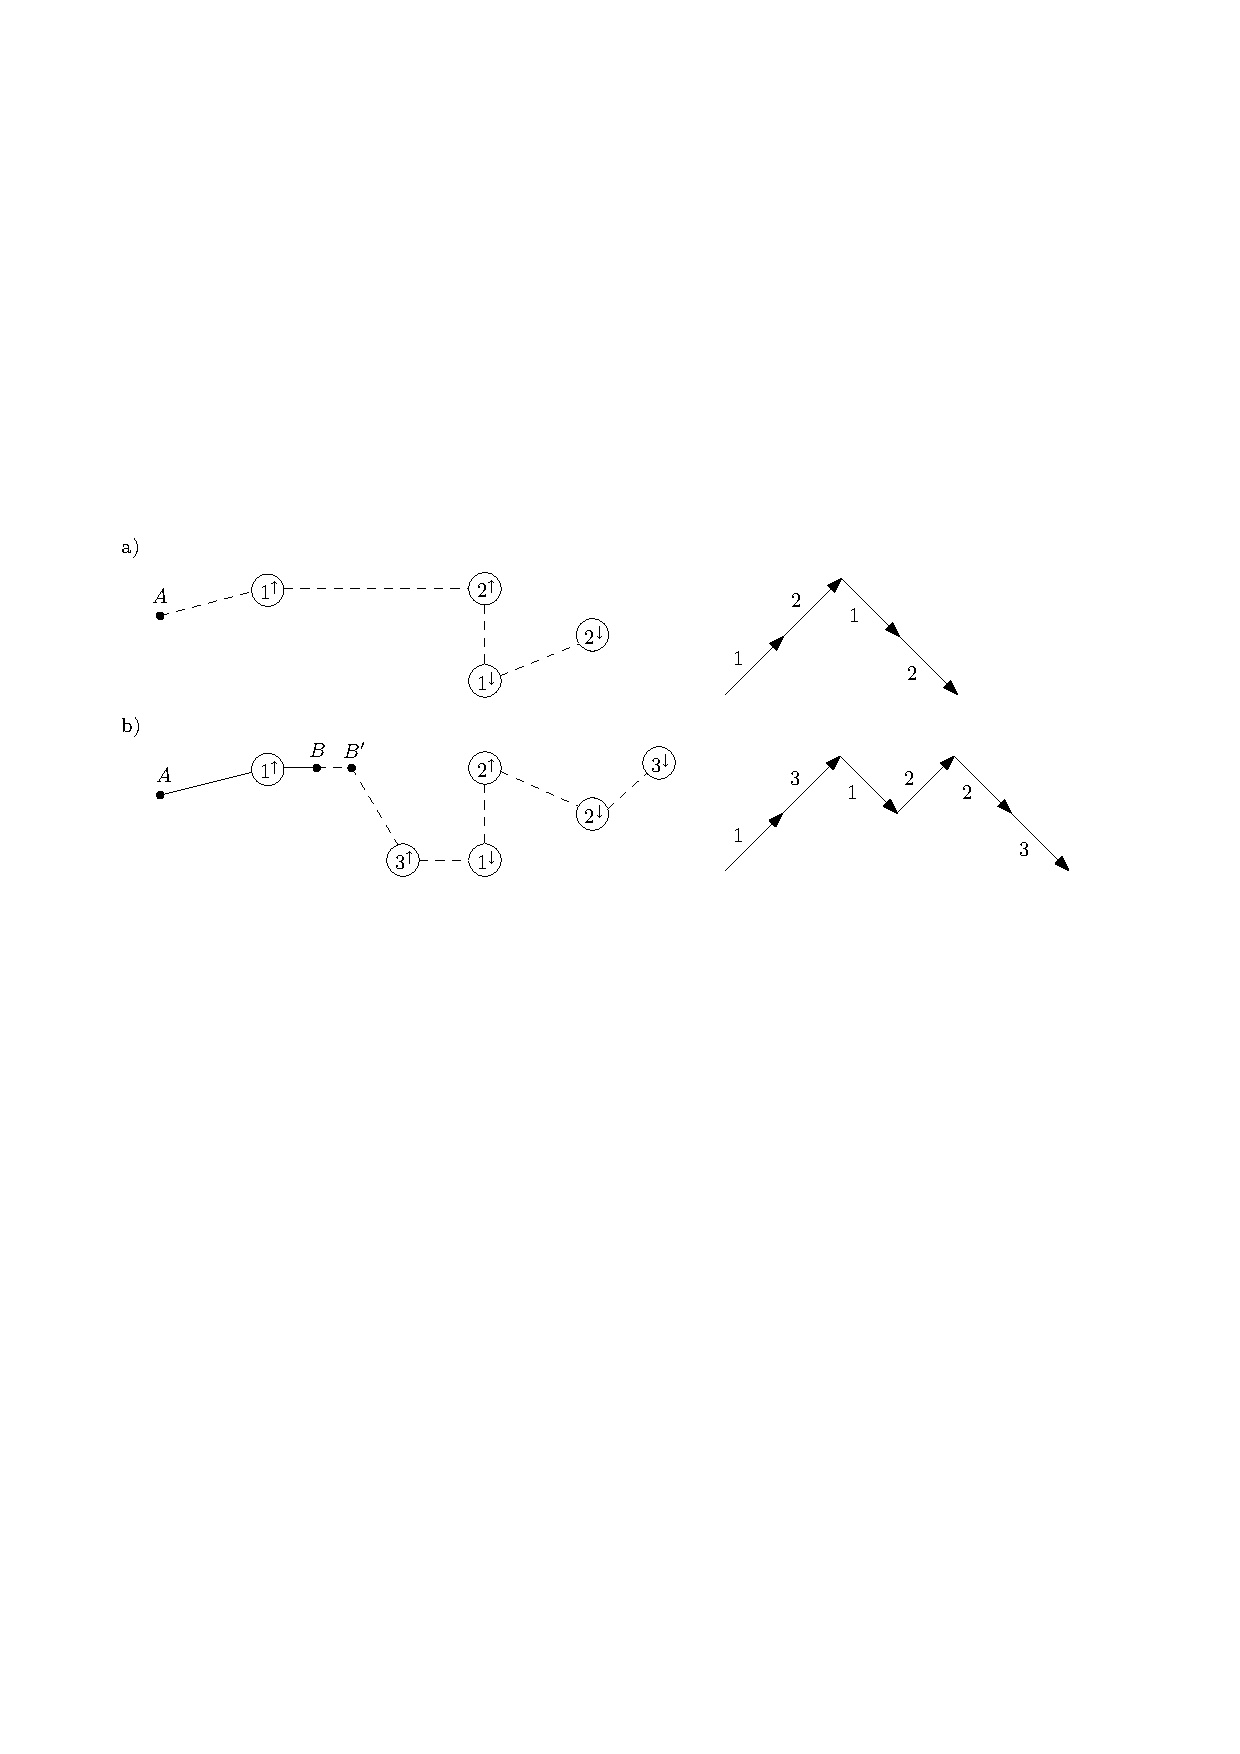
\includegraphics[width=1.0\textwidth]{dynamicexample04.pdf}
\caption{Modifications in the vehicle route. The route is updated when the vehicle is at $B$ and 
a new tentative optimal route beginning at $B'$ is produced. 
The figures on the right show the routes as so-called labeled Dyck 
paths \cite{cori}, in which each pick-up $i^{\uparrow}$ precedes the correspoding drop-off $i^{\downarrow}$. 
At the time a new customer is added to the route, a new path is formed. Clearly, the "height" of the path
shows the number of customers aboard in different parts of the route.}
\label{dynamicexample02}
\end{center}
\end{figure}

Note that the new route does not have $B$ as origin, but
a point $B'$, slightly ahead of $B$. This is due to two facts:
i) It will take some time for the algorithm to process the new input and reoptimize, 
ii) It will take some time for the driver
of the vehicle to process the information regarding the new route. 
The distance between $B$ and $B'$ depends in general on the particular 
dial-a-ride service examined. For example, in a highly dynamic setting,
in which the modification of the route is not
allowed to take more than a few seconds, it may be assumed that
the latter of the facts is more restrictive. 
Any dynamic dial-a-ride
service should make use of a mechanism to update the point $B'$
and estimated time of arrival $T'$ at $B'$ at sufficient time intervals.
The \emph{vehicle checkpoint} $(B',T')$ acts as the starting point for all service sequences.

	In addition, for customers that have already been picked up, the pick-up point 
	is not a part of the input of the problem. Thus, for such customers
	only the delivery point is considered.

	In dynamic models, the objective function
	used to find the solution over a rolling horizon has often little to do with
	the measures developed to evaluate the overall quality of a solution \cite{powell95}.
	However, the adaptive insertion method described in \ref{jeadarp} is designed in a way that several objective 
	functions, that are thought to be suitable
	for dynamic settings, may be incorporated with minimal work.
	Generally, the choice of the objective function depends 
	on the particular version of the dynamic routing problem and the performance
	of different objective functions may be sensitive to, for example, constraints, demand intensity
	or the number of vehicles. For a study related to choosing an objetive function
	for the immediate-request DARP, the reader is referred to \ref{csimutools}.


\subsection{Adaptive insertion algorithm [\citepub{jeadarp}]}
In general, exact procedures for solving routing  
problems are computationally very taxing, since the complexity is always more or 
less equal to the classical traveling salesman problem.
In addition, exact optimization can be seen to be needless at run-time if routes are modified often. 
Despite these facts, exact algorithms are useful in a way that the 
performance of different heuristics may be compared to the optimal solution. 

The main idea in the algorithm presented in \citepub{jeadarp} is that customers are added to 
the vehicle route one by one by using an \emph{exhaustive insertion} method,
which leads to a globally optimal solution, that is a vehicle route 
which is feasible with respect to all customers and minimizes a given cost function. 

Many studies related to the dial-a-ride problem, see for example \cite{jaw,madsen,diana,wong},
make use of what is called the insertion procedure, in the classical version of which   
the pick-up and delivery node of a new customer are inserted into the 
\emph{current optimal sequence} of pick-up and delivery nodes of existing customers.
In these references, several improvements to the insertion algorithm 
have been suggested. However, the main idea of the classical insertion algorithm a priori
excludes the possibility that the appearance of a new customer may render
the optimal sequencing of already existing customers no longer optimal.
While the basic insertion algorithm can be seen to
produce relatively good results for unconstrained problems, 
the performance compared to an exact algorithm is decreased as the
problem becomes more constrained.

The main idea is to construct the optimal route iteratively by implementing 
an insertion algorithm for each customer, one by one \emph{for all feasible sequences 
of pick-up and delivery nodes of existing customers}.
Namely, the procedure involves two steps for each customer:
\begin{enumerate}
	\item 
	Perform insertion of the new customer to all feasible service sequences with respect to
	existing customers.
	\item
	Determine the set of feasible service sequences with respect to the new customer and existing customers.
\end{enumerate}

It can be readily shown that the insertion of a new customer to all feasible service sequences with respect to 
existing customers 
produces all feasible service sequences with respect to the union of existing customers 
and the new customer and leads to a globally optimal solution but is computationally expensive
if the number of feasible service sequences grows large. However, if the route is constructed under relatively narrow time window constraints,
the number of feasible routes with respect to all customers
will be small compared to the number of all legitimate routes. 
Furthermore, the algorithm is easily extended to an adjustable heuristic algorithm
capable of handling any types of time windows. 

The idea of the advanced insertion method is 
clarified by the following example, where no
capacity or time constraints are taken into account. 
Let $i^{\uparrow} = i$ denote the \emph{pick-up node} of customer $i$ and let $i^{\downarrow} = N + i$ denote 
the \emph{delivery node} of customer $i$.
A \emph{service sequence} is defined as an ordered list consisting of pick-up and delivery nodes.
For instance, the service sequence $( i^{\uparrow},  j^{\uparrow}, j^{\downarrow}, i^{\downarrow})$ indicates the order
in which customers $i$ and $j$ are picked up and dropped off.

Let us start the advanced insertion process with customer 1.
Since the pick-up $1^{\uparrow}$ of customer 1 has to be before the delivery, $1^{\downarrow}$, 
the only possible service sequence at this point is $( 1^{\uparrow},  1^{\downarrow})$. Thus, the 
set of potential service sequences with respect to customer $1$ consists of this single service sequence. 
By insertion of customer $2$ into the service sequence $( 1^{\uparrow}, 1^{\downarrow})$ we get the six 
service sequences presented in table \ref{ykskakstaulukko01}.
\begin{table}[ht] 
\caption{Potential service sequences with respect to customers 1 and 2. 
No capacity or time constraints are taken into account. 
$i^{\uparrow}$ denotes the pick-up node and $i^{\downarrow}$ denotes
the delivery node of customer $i$.} 
\centering     
\begin{tabular}{|rrrrrr|rrrrrr|rrrrr|}  
\hline  & & & & & & & & & & & &  & & & &  \\ [-0.7em]                
A: & $ 1^{\uparrow} $ & $  1^{\downarrow} $ & $  2^{\uparrow} $ & $  2^{\downarrow} $ & & 
B: & $ 1^{\uparrow} $ & $  2^{\uparrow} $ & $  1^{\downarrow} $ & $  2^{\downarrow} $ & & 
C: & $ 1^{\uparrow} $ & $  2^{\uparrow} $ & $  2^{\downarrow} $ & $  1^{\downarrow} $ \\ [1ex]
\hline & & & & & & & & & & & &  & & & &  \\ [-0.7em]
D: & $ 2^{\uparrow} $ & $  1^{\uparrow} $ & $  1^{\downarrow} $ & $  2^{\downarrow} $ & & 
E: & $ 2^{\uparrow} $ & $  1^{\uparrow} $ & $ 2^{\downarrow} $ & $  1^{\downarrow} $ & & 
F: & $ 2^{\uparrow} $ & $  2^{\downarrow} $ & $  1^{\uparrow} $ & $  1^{\downarrow} $ \\ [1ex] 
\hline                      
\end{tabular} 
\label{ykskakstaulukko01} 
\end{table} 


By inserting the pick-up and delivery node of customer $3$ into all of these service sequences we get a total
of $6(5+4+3+2+1) = 90$ new potential service sequences. However, if the time and capacity
constraints are taken into account, not all service sequences described above are necessarily feasible.

For example, if after the insertion of customer $2$ it can be seen that only the
service sequences A and B in table \ref{ykskakstaulukko01}, namely 
$( 1^{\uparrow}, 1^{\downarrow}, 2^{\uparrow}, 2^{\downarrow})$ and $( 1^{\uparrow}, 2^{\uparrow}, 1^{\downarrow}, 2^{\downarrow})$,
are feasible with respect to time constraints, then it can be
shown that all feasible service sequences including customer $3$ are included in
the sequences given by insertion to these two service sequences, which gives
a maximum of $2(5+4+3+2+1) = 30$ new potential service sequences.

Briefly, the structure of the advanced insertion algorithm may be sketched as follows.
At first, the set of feasible service sequences $S_i$ is determined recursively
for each customer $i \in \{1, \ldots, N\}$ by inserting the pick-up and delivery nodes of customer $i$ into each feasible
service sequence with respect to customers $1,\ldots,i-1$. In this way the algorithm 
produces the set $S_N$ of all feasible routes with respect to customers $1,\ldots,N$. 
Then the solution to the static problem is obtained by choosing the sequence $s \in S_N$ with
minimal cost $C(s)$. In the general form \eqref{tavoitefunktio01} of the cost function, this involves
the calculation of waiting times and ride times for all customers
for all feasible service sequences. If only route duration is minimized,
we can simply choose the sequence for which the arrival time at the last
node is smallest.


\subsubsection{A priori clustering}
\label{clustering}
In problems involving a large number of customers, assuming that the time windows are relatively narrow,
a significant portion of service sequences can be eliminated before 
the actual insertion process by simply studying the mutual relationships between nodes, similarly 
as described in \cite{dumas03}.
More precisely, assume that the vehicle departs from a node $i$ at the lower
bound $E_i$ of the time window and moves directly to node $j$. If the vehicle 
does make it in time to $j$, that is, if
	\begin{align}
		E_{i} + t(i,j) & > L_{j},
	\end{align}
it is said that the transition $i\to j$ is \emph{a priori infeasible}.

Note that if for any two nodes $i$ and $j$, both transitions $i \to j$ and 
$j \to i$ are infeasible a priori, the entire problem is infeasible. 
Otherwise, either $i \to j$ or $j \to i$ or both are a priori feasible and the pick-up and delivery nodes of customers
can be divided among $m$ preceding clusters by using the following rule.

\begin{definition}
Cluster $C_k$ precedes cluster $C_l$ 
if and only if the transition $x \to y$ is a priori infeasible for all $x \in C_l$ and
$y \in C_k$. In this case, we shall use the notation $C_k \prec C_l$.
\end{definition}

Clearly, assuming that there exists a feasible solution, the above precedence relation 
of clusters is a strict order: (i) $C \not\prec C$ for all clusters, (ii) $C_a \prec C_b$
implies $C_b \not\prec C_a$ and (iii) $C_b \prec C_c$ and $C_a \prec C_b$ implies
$C_a \prec C_c$. In addition, note that if a single node $i$ has an infinite time window $[-\infty,+\infty]$, there is 
only one cluster since all transitions $j \to i$
and $i \to j$ are feasible a priori.

The clusters can be illustrated by means of an adjacency matrix $F$ for which $F_{ij}=1$ if $i\to j$ is
feasible and $F_{ij}=0$ if $i\to j$ is infeasible a priori. By arranging the rows and
columns suitably we get a block upper triangular matrix where each block corresponds to
a cluster. Figure \ref{clusterexample01} shows the adjacency matrix of a sample problem
involving four customers. The rows and columns are arranged in a descending order 
with respect to row sums. From the matrix five clusters can be identified (blocks on the diagonal), namely 
$\{1^{\uparrow} \}	\prec \{ 1^{\downarrow}, 3^{\uparrow}, 2^{\uparrow}\} \prec \{ 2^{\downarrow} \} \prec  
\{ 3^{\downarrow}, 4^{\uparrow} \} \prec  \{ 4^{\downarrow} \}$. 
Thus, since the positions of nodes $1^{\uparrow}, 2^{\downarrow}$ and $4^{\downarrow}$ are fixed,
the problem falls down to determining the 
optimal ordering of nodes $1^{\downarrow}, 3^{\uparrow}, 2^{\uparrow}$ and 
$3^{\downarrow}, 4^{\uparrow}$. 
\begin{figure}[ht]
\begin{center}
\begin{align*}
\newcommand*{\temp}{\multicolumn{1}{c|}{0}}
\newcommand*{\tempi}{\multicolumn{1}{c|}{1}}
\begin{array}{c|cccccccc}
   & 	1^{\uparrow}	   &  1^{\downarrow}   &  3^{\uparrow}   &  2^{\uparrow}   &  2^{\downarrow}   &  3^{\downarrow}   &  4^{\uparrow}   &  4^{\downarrow} \\
   \hline
1^{\uparrow} &     1   &  1   &  1   &  1   &  1   &  1   &  1   &  1 \\ \cline{2-2}
1^{\downarrow} &     \temp   &  1   &  1   &  1   &  1   &  1   &  1   &  1 \\
3^{\uparrow} &     \temp   &  1   &  1   &  1   &  1   &  1   &  1   &  1 \\
2^{\uparrow} &     \temp   &  1   &  1   &  1   &  1   &  1   &  1   &  1 \\ \cline{2-5}
2^{\downarrow} &     0   &  0   &  0   &  \temp   &  1   &  1   &  1   &  1 \\ \cline{2-6}
3^{\downarrow} &     0   &  0   &  0   &  0   &  \temp   &  1   &  1   &  1 \\
4^{\uparrow} &     0   &  0   &  0   &  0   &  \temp   &  1   &  1   &  1 \\ \cline{2-8}
4^{\downarrow} &     0   &  0   &  0   &  0   &  0   &  0   &  \temp   &  1 \\ \cline{2-8}
\end{array}
\end{align*}
\caption{A priori adjacency matrix of a sample problem involving $4$ customers. From the matrix five clusters can be identified, namely 
$\{1^{\uparrow} \}	\prec \{ 1^{\downarrow}, 3^{\uparrow}, 2^{\uparrow}\} \prec \{ 2^{\downarrow} \} \prec  
\{ 3^{\downarrow}, 4^{\uparrow} \} \prec  \{ 4^{\downarrow} \}$.}
\label{clusterexample01}
\end{center}
\end{figure}
In general, by clustering the nodes a priori, a significant amount
of insertions need not be checked for feasibility. 


\subsubsection{Structure and complexity}
The number of insertions that are tested for feasibility for customer $i$ is bounded above 
by the formula
\begin{align}
n(i) \leq m_{i-1} \sum_{x=1}^{2i-1} x  = \frac{m_{i-1}(2i)(2i-1)}{2},
\end{align}
where $m_{i-1}$ is the number of feasible service sequences with respect to customers $1, \ldots,i-1$.
The inequality can be justified by the fact that not all possible insertions  
are checked for feasibility. 
In the worst case, where capacity and time constraints are \emph{not restrictive},
we get 
\begin{align*}
& m_1 = 1, \ \ \ \ \ \ \ m_2 = (4 \cdot 3)/2 = 6,  \ \ \ \ \ \ \ m_3 = 6(6 \cdot 5)/2 = 90, \\
& m_i = \frac{(2i)(2i-1)}{2} \frac{(2(i-1))(2(i-2)-1)}{2} \cdots \frac{4 \cdot 3}{2} = \frac{(2i)!}{2^i}. 
\end{align*}
Thus the maximum number of insertions required in the solution of the static case is
$\sum_{i=1}^{N}\frac{(2i)!}{2^i} \approx \sum_{i=1}^{N} {2^{1-i} i^{2i + \frac 12} \sqrt{\pi}}$.
Thus, in the worst case, the number of feasible solutions is of order
$\mathcal{O}(\sqrt{N} (N^2/2)^N)$.

Suppose that, due to strict time (and capacity) constraints, the number of potential service sequences $m_i$ for customers $1,\ldots, i$
is bounded by some function $m:\mathbb{N} \to \mathbb{N}$ such that $m(i) \leq \frac{(2i)!}{2^i}$.
Then the number of insertions for customer $i$ is bounded by $n(i) \leq \frac{m(i-1)(2i)(2i-1)}{2}$.
The total number of insertions is bounded by $\sum_{i=1}^{N}\frac{m(i-1)(2i)(2i-1)}{2}$.
For example, if $m(i) = kN$ for some constant $k$, the computational complexity of the screening phase
is reduced to $\mathcal{O}(N^4)$. 
If $m(i) = k$, the computational complexity is reduced to $\mathcal{O}(N^3)$.

On the grounds of previous calculations, it can be stated that if the number
of feasible service sequences is bounded due to strict constraints, the 
algorithm will lead to an exact solution computationally inexpensevely.
In addition, the 
algorithm has a special property of being extendable to an adjustable heuristic,
as described in the following section.

\subsubsection{A heuristic extension}
\label{svheuristic}
Even if the capacity and time constraints were not highly restrictive, the algorithm can be 
modified easily by bounding the size of the set $S_i$ 
of service sequences, in which new customers are inserted, 
by including only a maximum of $L$ service sequences
for each customer $i$. More precisely, if after inserting 
customer $i$, the number of feasible service sequences with respect to customers $1,\ldots, i$
is larger than $L$, the set of feasible service sequences $S_i$ with respect to 
customers $1,\ldots, i$ is narrowed by including only $L$  
service sequences, that seem to allow the insertion of remaining customers.
After the last customer has been inserted, the feasible service sequences are evaluated
by means of the objective function \eqref{tavoitefunktio01}.

This modification leads to a heuristic algorithm, in which the computational
effort can be controlled by the parameter $L$, referred to as the \emph{degree} of
the heuristic. The resulting algorithm is
somewhat sophisticated in a way that it produces globally optimal solutions for
small sets of customers and when the number of customers is increased, the
algorithm still produces locally optimal solutions with 
reasonable computational effort. In the special case where $L=1$, the
algorithm reduces to the classical insertion algorithm. 
If $L \geq \frac{(2N)!}{2^N}$, the heuristic coincides with the exact version of the 
algorithm as no routes are discarded.

\subsubsection{Objective functions}
\label{hobjfunc}
In order to be able to efficiently make use of the above heuristic extension
idea, the set of service sequences is narrowed by means of a certain heuristic objective function
after the insertion of each customer.
Since the main purpose of heuristics at the operational level is to always produce some implementable 
solutions very quickly, even if they were only locally optimal, such an objective function should 
be defined in a way that the algorithm is 
capable of producing \emph{feasible} solutions even if the complexity of the problem was high. %was highly constrained.

Looking only at the cost defined in formula \eqref{tavoitefunktio01} may eliminate from consideration
sequences that are marginally costlier but would easily allow the
insertion of remaining customers in the route. 
Thus, more sophisticated criteria should be considered to help ensure that the heuristic will
find a feasible solution when one exists.

In other words, the function should favor service sequences with enough 
\emph{time slack} for those customers, that have not been inserted into the sequences.
\ref{jeadarp} suggests the following heuristic objectives.
Given the service sequence $s = (p_1, \ldots, p_{m})$, we wish to optimize one 
of the functions 
\begin{align}
\label{rl}
f_{rl}(s) &= t_m, & \mbox{(Route duration)} \\
\label{ts}
f_{ts}(s) & = \sum_{j=1}^{m} L_j -t_j ,  & \mbox{(Total time slack)} \\
\label{maxmin}
f_{min}(s) &= \min_{j \in \{1, \ldots, m\}}  L_j - t_j, & \mbox{(Max-min time slack)} 
%\label{lastnode}
%f_{LN}(s) &= L_m - t_m, & \mbox{(Last node time slack)} 
\end{align}
where $[E_j,L_j]$ is the time window and $t_j$ is the calculated time of arrival at node $p_j$.

In general, each of the above objective functions aim to 
maximize the temporal flexibility of service sequences in different ways.
\begin{description}
\item[Route duration]
%The route duration objective function 
\eqref{rl} favors service sequences in
which the time to serve all customers is as small as possible. 
This objective can be justified by the fact that 
it is likely that new customers may be inserted at the rear of 
a route that is executed quickly.
\item[Total time slack] 
\eqref{ts} stores sequences in which
the sum of excess times (or the average excess time) at the nodes is maximized, that
is, sequences which are likely to allow the insertion of a new customer %can be inserted
before the last node.
\item[Max-min] \eqref{maxmin} seeks sequences in which the 
minimum excess time at the nodes of the route is maximized. In other words,
the sequences in which there is at least some time slack at each node
are considered potential.
\end{description}

A simple example motivating the use of the above objective functions is 
presented in figure \ref{flexibility01}.

\begin{figure}[ht]
\begin{center}
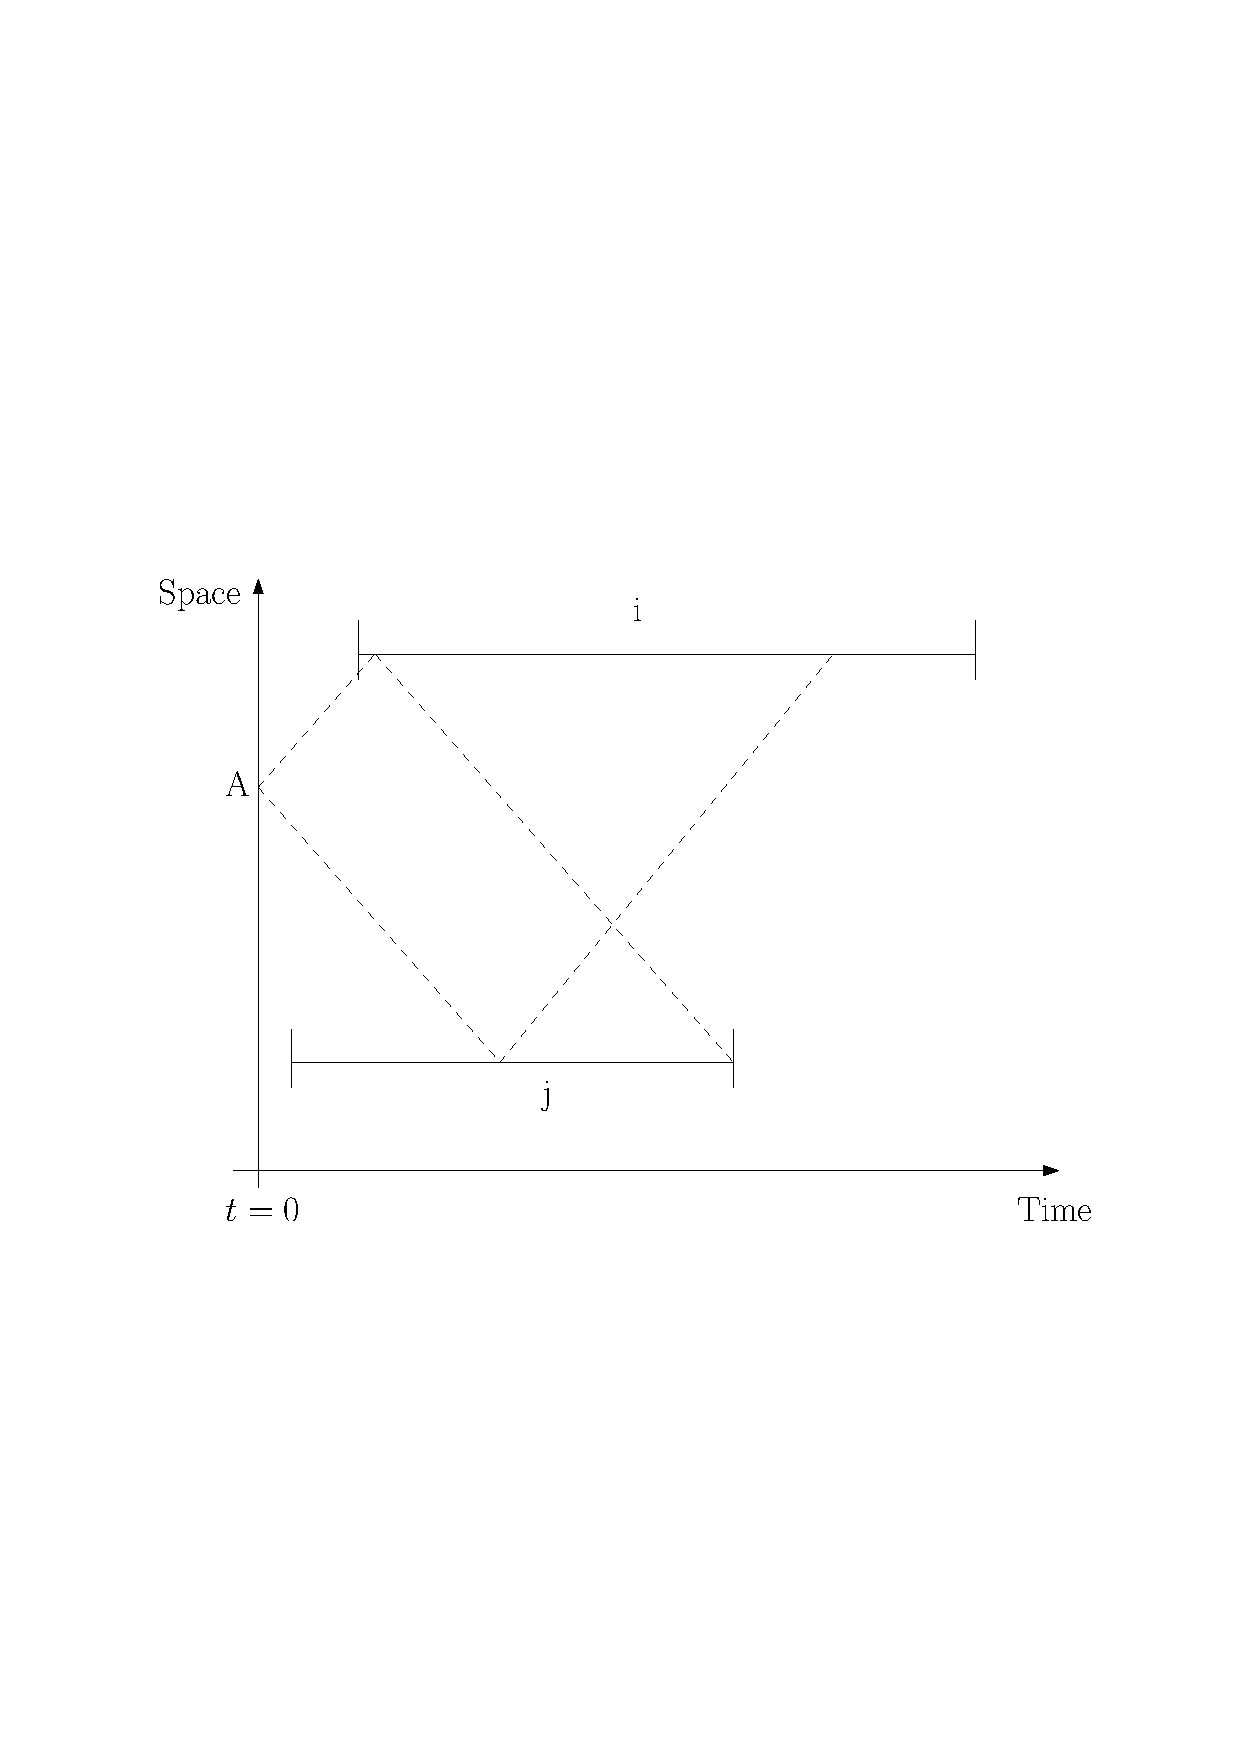
\includegraphics[width=0.9\textwidth]{flexibility03.pdf}
\caption{Route flexibility. A vehicle is located at $A$ at $t = 0$,
and two customers are due to be picked up within the presented time windows at $i$ and $j$.
The dashed lines represent two possible routes for the vehicle.
If the route duration were minimized, $i$ should be visited before $j$. However, since
there would be no "slack time" at $j$, this decision would a priori 
exclude the possibility that new customers could be inserted between $i$ and $j$. 
On the other hand, if $j$ were visited before $i$, there would be
more possibilities for inserting new customers on the route before $i$. However, 
the route $A \to i \to j$ is shorter and thus it is more likely that 
customers can be inserted at the end of the sequence.}
\label{flexibility01}
\end{center}
\end{figure}



\subsubsection{Tuning}% $K$-multiplying}
\label{doubling}
In order to ensure that the heuristic always produces a feasible solution when one exists,
the parameter $L$ can be tuned during run-time by using the following idea. 
\begin{enumerate}
\item
At first, the problem is solved by using an initial degree $L_0$. 
\item
Each time the algorithm is unable to find a feasible solution, the degree is increased and 
the problem is solved again.
\end{enumerate}
Let us study the expected CPU time of the tuning method described above.
Let $P(S|L=l)$ denote the probability that a solution is found by using the degree $L=l$
and let $T(l)$ denote the average running time of the algorithm with $L=l$. 
The expected CPU time for a given tuning strategy $(L_0,L_1,\ldots)$, where $L_0 < L_1 < L_2 < \ldots$, 
is given by the formula %can be written in the form
\begin{align*}
%E(\tau(\textbf{L})) & = 
T(L_0) + \sum_{i=1}^{\infty} T(L_i) \prod_{j=0}^{i-1} (1- P(S|L=L_i)). 
\end{align*}
It should be noted that the above probabilities are actually conditional: If a solution
is not found with some value of $L$, there is no point in solving the problem 
again with the same value. In addition, a relatively small increase in 
the value of $L$ will not significantly affect the possibilities
of finding a solution. Thus, the tuning approach used in the following examination
is based on multiplying the value of $L$ by a number $K$ each time a feasible
solution is not found. This method will be referred to as $K$-multiplying.

Assuming that %for sufficiently small values of $l$, 
the complexity grows linearly with $l$, that is $T(l) = l T(1)$, and %, which implies that $E(\tau(L_0)) \geq T(L_0)$. 
that the probability of finding a solution is sufficiently high, %$1/2 < P(S|L=1) < P(S|L=2) < \ldots$, 
it can be shown that the optimal initial degree
for the $K$-multiplying method has to be relatively small. %is $L_0=1$. 
At first we will show %, for the $K$-multiplying method, where $K \geq 2$ is a natural number, 
that if $P(S|L \geq 1)>1/2$, then %and $k=2$ corresponds to the doubling method, 
any initial degree $L_0 = mK$, where $m \in \mathbb{N}$, is suboptimal. %the optimal value satisfies $1 \leq L_0 < k$,

\begin{theorem}
\label{doublingthm01}
Let $E(\tau(L_0))$ denote the expected CPU time of the $K$-multiplying method for the initial value $L_0$. If
$T(l) = l T(1)$ for $l \in \mathbb{N}$ and $P(S|L \geq 1) > 1/2$, then
\begin{align*}
E(\tau(L_0)) \leq E(\tau(KL_0))
\end{align*}
for all $L_0 \in \mathbb{N}$ and $K \geq 2$.
\end{theorem}
Then, the following theorem states that if the probability of finding a solution
is at least $1 - 1/K$, the optimal initial value is 
bounded above by the logarithm of the smallest natural number $l$ for which $P(S|L=l)=1$.

\begin{theorem}
\label{doublingthm02}
Let $l'$ denote the smallest natural number $l$ for which $P(S|L=l)=1$.
If $P(S|L \geq 1) > 1 - 1/K$, then 
\begin{align*}
E(\tau(L_0)) < T(L_0(1+\log_K l'/L_0))
\end{align*}
for all $L_0 \in \mathbb{N}$ and for all $K > 1$.
\end{theorem}

In general, the two theorems (for proofs, see \ref{jeadarp}) suggest that the expected 
CPU time is minimized when the initial degree $L_0$ is small. 
For example, if $l' = 16$ , $K=2$ and $P(S|L \geq 1) > 0.5$, theorem \ref{doublingthm02} states that
that $E(\tau(1)) < T(5)$. By theorem \ref{doublingthm01} we know that
the values $2$ and $4$ are suboptimal for $K=2$. Thus, the optimal initial value
is either $1$ or $3$ depending on the actual probabilities of finding solutions with different values of $L$. 

Finally, it should be noted that 
by increasing the values of $K$ and $L_0$, the optimality of the 
solution with respect to the objective of the problem is increased as well since more sequences are evaluated.

\subsection{Routing by ranking [\citepub{jrbrorl}]}
\label{routingbyranking}
Several web information retrieval (IR) methods have been developed
for finding the most appropriate web pages corresponding to 
queries given to search engines. The most sophisticated methods, such as HITS \cite{kleinberg}, PageRank \cite{brin01} and SALSA \cite{lempel}
in use today make use of the hyperlinked structure of the web, since
the goodness of a web page and the position of the page with respect to
other web pages seem to have a certain connection. 
For example, a web page may be
considered good if there are many other web pages linking to that page. In other words, 
web pages are ranked by search engines not only by means of the content of the page, but
also by exploiting information regarding the hyperlink-induced relationships between pages.

The bringing of hyperlinks to bear on the ordering of web pages has given rise to
a mathematical analysis related to hyperlink-induced web IR methods, such as in
\cite{farahat, langville, ng, agosti}, in which the 
behaviour of several IR methods is studied from the computational point of view.

The HITS (Hyperlink-Induced Topic Search) algorithm defines \emph{authorities} 
(web pages with several inlinks) and \emph{hubs} (several outlinks). 
The HITS thesis is that \emph{good hubs point to good authorities and good authorities
are pointed to by good hubs}. Based on this thesis, both a hub score and an authority score is assigned to
each web page \cite{langville}. 

\ref{jrbrorl} presents an application of HITS on the dial-a-ride problem (DARP)
\cite{berbegliathesis,berbegliahybrid,berbegliafeas}.
Here the DARP is examined as a \emph{constraint satisfaction problem}, in which the goal
is to find a feasible vehicle route that serves all customers, or to maximize the number of served customers.

In the context of the dial-a-ride problem, 
the links between nodes are defined as feasible transitions with respect to the %time, capacity and precedence 
constraints of the problem: If node $j$ can be visited after $i$, a link from $i$ to $j$ 
is formed. Thus, a good hub score of a pick-up or drop-off node $i$ means 
that many nodes can be reached in time from $i$. 
Thus, in order to efficiently find feasible solutions to the dial-a-ride problem, we suggest that nodes with large 
hub scores should be visited first since there are many nodes that can
be visited after such nodes. 


\subsubsection{The HITS algorithm \cite{kleinberg}}
\label{hits}
Given a web graph $G = (V,A)$ consisting of pages $V$ and links $A$ between pages,
the authority and hub scores $a_i$ and $h_i$ are computed for each page $i$ as follows.
Letting 
$(i,j)$ represent a link from page $i$ to page $j$, given that each page has been 
assigned an initial authority score $a_i(0)$ and hub score $h_i(0)$, HITS successively
refines these scores by computing
\begin{align*}
a_i(k) & = \sum_{(j,i) \in A} h_j(k-1) \\
h_i(k) & = \sum_{(i,j) \in A} a_j(k-1)
\end{align*}
for $k \in \{1,2,\ldots\}$. By using matrix notation, these equations can be written the form 
$a(k) = L^T h(k-1)$ and $h(k) = L a(k-1)$,
where $a(k)$ is the authority vector containing the authority scores of
each of the pages at step $k$, $h(k)$ is the corresponding hub vector and
$L$ is the adjacency matrix of the graph with elements $L_{ij} = 1$ if
$(i,j) \in A$ and $L=0$ otherwise \cite{langville}. 

It has been shown in \cite{farahat} that the authority and hub vectors
describing the authority and hub scores of nodes of a given graph are given by 
the dominant eigenvectors of the matrices $L^TL$ and $LL^T$ 
(or equivalently, dominant singular vectors of $L$), 
where $L$ is the adjacency matrix of the graph. 
%Thus the authority and hub
%scores may be efficiently calculated by using eigenvalue (or singular value) algorithms. 

\subsubsection{Modified HITS}
\label{modifiedhits}
For constrained routing problems, a modified version of the HITS algorithm is used, in which only the hub scores
are considered. More precisely, the thesis is that \emph{good hubs point to good hubs}. 
This formulation is motivated by Theorem \ref{polut}, which states that for a specific class of graphs,
the hub score of a node $i$ corresponds to the number of self-avoiding paths
from $i$ to a given destination node.
When attempting to construct a path that visits all nodes, or to maximize the number of visited nodes, 
the modified HITS idea induces the following intuitive policy: 
Good hubs are visited first, since many nodes can be reached from good hubs. 

The hub scores are calculated as follows.
Let $L$ denote the adjacency matrix of a directed graph $G$. 
Similarly as in the HITS algorithm, the hub vector containing the \emph{hub scores} of nodes is first initialized, $h(0) = (1,1,\ldots,1)$ 
and the hub vector is successively updated by means of the power method
\begin{align}
\label{modhub}
h'(k) & = L h(k-1).
\end{align}
Similarly as in the original HITS algorithm, the hub vector
converges to a dominant eigenvector of $L$.

Theorem \ref{polut} characterizes the hub scores produced by the modified HITS algorithm for 
\emph{sink graphs} defined as follows.
\begin{definition}
  Let $G=(V,A)$ be a directed acyclic graph and let $s \in V$ be a node such that $(s,i) \notin A$ for all $i \in V$.
The graph $G_s=(V, A \cup (s,s))$ is called a \emph{sink graph}. 
\end{definition}
In other words, a sink graph is a directed acyclic graph $(V,A)$ with the exception that one node $s \in V$ with zero outdegree is
associated with a loop $(s,s)$.

\begin{theorem}
\label{polut}
Let $L$ denote the adjacency matrix of a sink graph $G_s=(V,A)$, where $V=\{1,\ldots,|V|\}$,  
let $h_i$ denote the number of self-avoiding paths from $i$ to $s$ for $i \in V \setminus \{s\}$ and let $h_s=1$. 
Then, $h=(h_1,\ldots,h_{|V|})^T$ is a unique dominant eigenvector of $L$.
\end{theorem}

Note that since $h_i \leq h_j$ for all $i,j \in V$ for which $L_{ij} = 1$, the vector $h$ defines a \emph{topological
ordering} \cite{cormen} of the nodes for which $h_i > 0$.
Although Theorem \ref{polut} considers a special class of 
graphs\footnote{The calculation of self-avoiding paths in graphs with cycles is discussed in \cite{ponstein}.}, 
the result gives us an idea of the behaviour of the modified HITS method: There are many paths beginning from 
nodes with high hub scores. 

In the following section, we show how the 
hub scores are used to give indicative guidance to 
a dynamic programming algorithm for the dial-a-ride problem.

\subsubsection{The ranking method}
\label{svsolution}
\ref{jrbrorl} presents an exact constraint programming method for the single-vehicle DARP that 
produces a feasible solution whenever one exists or proves that the problem is infeasible.
In the latter case, the algorithm returns a route that maximizes the number of served customers.
The main challenge is to find a sequence of pick-up and drop-off nodes for which 
the time and precedence constraints are satisfied. While capacity constraints are 
also considered, the focus is on problems, in which time limits are more restrictive.

Letting node $0 \in V$ be the location of the vehicle at $t=0$,
we aim to find a feasible path $(0,p_1,\ldots,p_{2n},0)$
consisting of the pick-up and drop-off nodes of $n$ customers.
The number of permutations is $(2n)!$ and the number of feasible permutations
with respect to precedence constraints is $(2n)!/2^n$, see \ref{jeadarp}.

Briefly, our approach to the problem is a \emph{depth-first} search, in which the
remaining nodes are ranked by means of hub scores at each step and the order of the depth-first search is determined by the 
ranking. %\footnote{This idea is remotely similar to lexicographic depth first search (LDFS) \cite{golumbic}.}.
The search begins from node $0$ by ranking the pick-up and drop-off nodes $P$ of all customers.
Then, the node $p^{*}$ with the highest ranking is added to the sequence and the ranking procedure is
repeated for the remaining nodes $P \setminus \{p^{*}\}$.

Formally, the search is executed by means of the recursion 
REC($S,R_S$) shown in Algorithm \ref{rralg}, where $S$ denotes a sequence of nodes (initially $S=(0)$), $R_S$ denotes %based on a two-step feasibility check 
the set of remaining nodes at $S$ (initially $R_S=\{1^{\uparrow},1^{\downarrow}, \ldots, n^{\uparrow},n^{\downarrow}\}$) and $S_{\max}$ denotes the sequence that maximizes the number 
of served customers (initially $S_{\max} = (0)$). $C(S)$ denotes the number of served customers in sequence $S$, which is equal to the 
number of drop-off points in $S$.
\begin{algorithm}
{\footnotesize
\begin{algorithmic}
\STATE Check time, capacity and precedence constraints;
\IF {$S$ is infeasible} 
\STATE \ \ Return;
\ENDIF
 \IF {$C(S) > C(S_{\max})$}
 \STATE \ \ $S_{\max} \leftarrow S$;   \hfill (Store the current sequence $S$.) %$C(S) = $ The set of served customers in sequence $S$)
 \STATE \ \ \textbf{if} $C(S) = n$
 \STATE \ \ \ \ Terminate recursion; \hfill (Feasible route.)
 \STATE \ \ \textbf{end if}
 \ENDIF
%\IF {$C(S) = n$}
%\STATE \ \ Terminate recursion; \hfill (Feasible route.)
%\ENDIF
\STATE Rank the remaining nodes $i \in R_S$ and remove infeasible nodes from $R_S$; 
\FOR{all $i \in R_S$ (in ranked order)}
\STATE \ \ REC$((S,i) , R_S \setminus \{i\})$; %\hfill ($R_{(S,i)}$ = the set of remaining nodes at $(S,i)$.) 
%\ELSE 
%\STATE \ \ \ \ $R = R \setminus \{i\}$; 
\ENDFOR
\end{algorithmic}
\caption{\footnotesize A recursive solution REC($S,R_S$) to the single-vehicle DARP. $S$ denotes a sequence of 
nodes (initially $S=(0)$), $R_S$ denotes %based on a two-step feasibility check 
the set of remaining nodes (initially $R_S=\{1^{\uparrow},1^{\downarrow}, \ldots, n^{\uparrow},n^{\downarrow}\}$) and $S_{\max}$ denotes the sequence that maximizes the number 
of served customers (initially $S_{\max} = (0)$). $C(S)$ denotes the number of served customers in sequence $S$, which is equal to the 
number of drop-off points in $S$.}
\label{rralg}
}
\end{algorithm}

The main idea of the recursion is that at each step, we have the current sequence $S$ 
and the set of remaining nodes $R_S$ (nodes that can possibly be added to the sequence). 
At first, we check the time, capacity and precedence constraints of $S$.
If $S$ is feasible and all customers have been served, that is, if $C(S) = n$, a feasible solution is found and 
the recursion is terminated.
Otherwise,
the remaining nodes $R_S$ are ranked by hub scores and the infeasible nodes 
are removed from $R_S$.
Then, the recursive function REC($(S,i),R \setminus \{i\}$) is called
for all sequences $(S,i)$ in ranked order.
In the following, we describe the ranking of remaining nodes in more detail.


\subsubsection{Hub scores}
\label{feasibility}
The ranking of the remaining nodes $R_S$ is determined in two phases: 
First, the adjacency matrix of the remaining nodes is determined by studying 
feasible transitions between the nodes.
Then, the hub vector is calculated by means of Equation \eqref{modhub}.

Given that the vehicle is at the last node $s$ of sequence $S$, we study which sequences $(S,i,j)$, where 
$i,j \in R_S$, are feasible with respect to the time and precedence constraints. %, capacity and precedence constraints. 
Let $t_s$ denote the departure time and $Q_s$ denote the load of the vehicle at $s$, 
and $t_i = t_s + T_{si}$ denote the arrival time at $i \in R_S$. For clarity, service times are 
assumed equal to zero. However, the modification
of the following equations for non-zero service times is straightforward.
In addition, we consider %The above definition of feasible transitions %\ref{feasibletransitions} 
fixed time windows $[E_i,L_i]$ for each node.
However, maximum ride time constraints \cite{hunsaker} are taken into account by updating the 
upper bounds $L_i$ of the time windows during run-time as described in \ref{jhitsdarpts}.

First, all nodes that are seen to be non-reachable from $S$ are removed from the set $R_S$ of remaining nodes.
\begin{definition}
 \label{linkki02}
A node $i \in R_S$ is said to be infeasible if
there does not exist a feasible sequence $(S,\ldots,i)$ ending at $i$.
\end{definition}
Clearly, if the time of arrival $t_i$ staisfies $t_i > L_i$, the node $i$ is infeasible.
The nodes $i \in I$ for which $t_i > L_i$ are removed from $R_S$, 
that is, $R_S \leftarrow R_S \setminus I$. This elimination criteria is similar to 
the one presented in \cite{desrosiers01}.

For nodes that are not seen to be infeasible, we define feasible transitions as follows.
\begin{definition}
\label{feasibletransitions}
The transition 
$i \to j$ from node $i \in R_S$ to node $j \in R_S$ is said to be \emph{feasible}, if 
$\max(t_i, E_i) + T_{ij} \leq L_j$. 
\end{definition}
The above definition is similar to the one studied in \cite{dumas03}, 
in which the set of \emph{admissible arcs} between the pick-up and delivery nodes is constructed
as a preprocessing step in the pickup and delivery problem. The set of admissible arcs is 
made up of arcs which a priori satisfy the precedence, capacity and time constraints of the problem.
The difference in \eqref{feasibletransitions} is that feasibility of 
transitions is defined as a function of the state of the vehicle (see Figure \ref{transitions01}).

\begin{figure}[ht]
\begin{center}
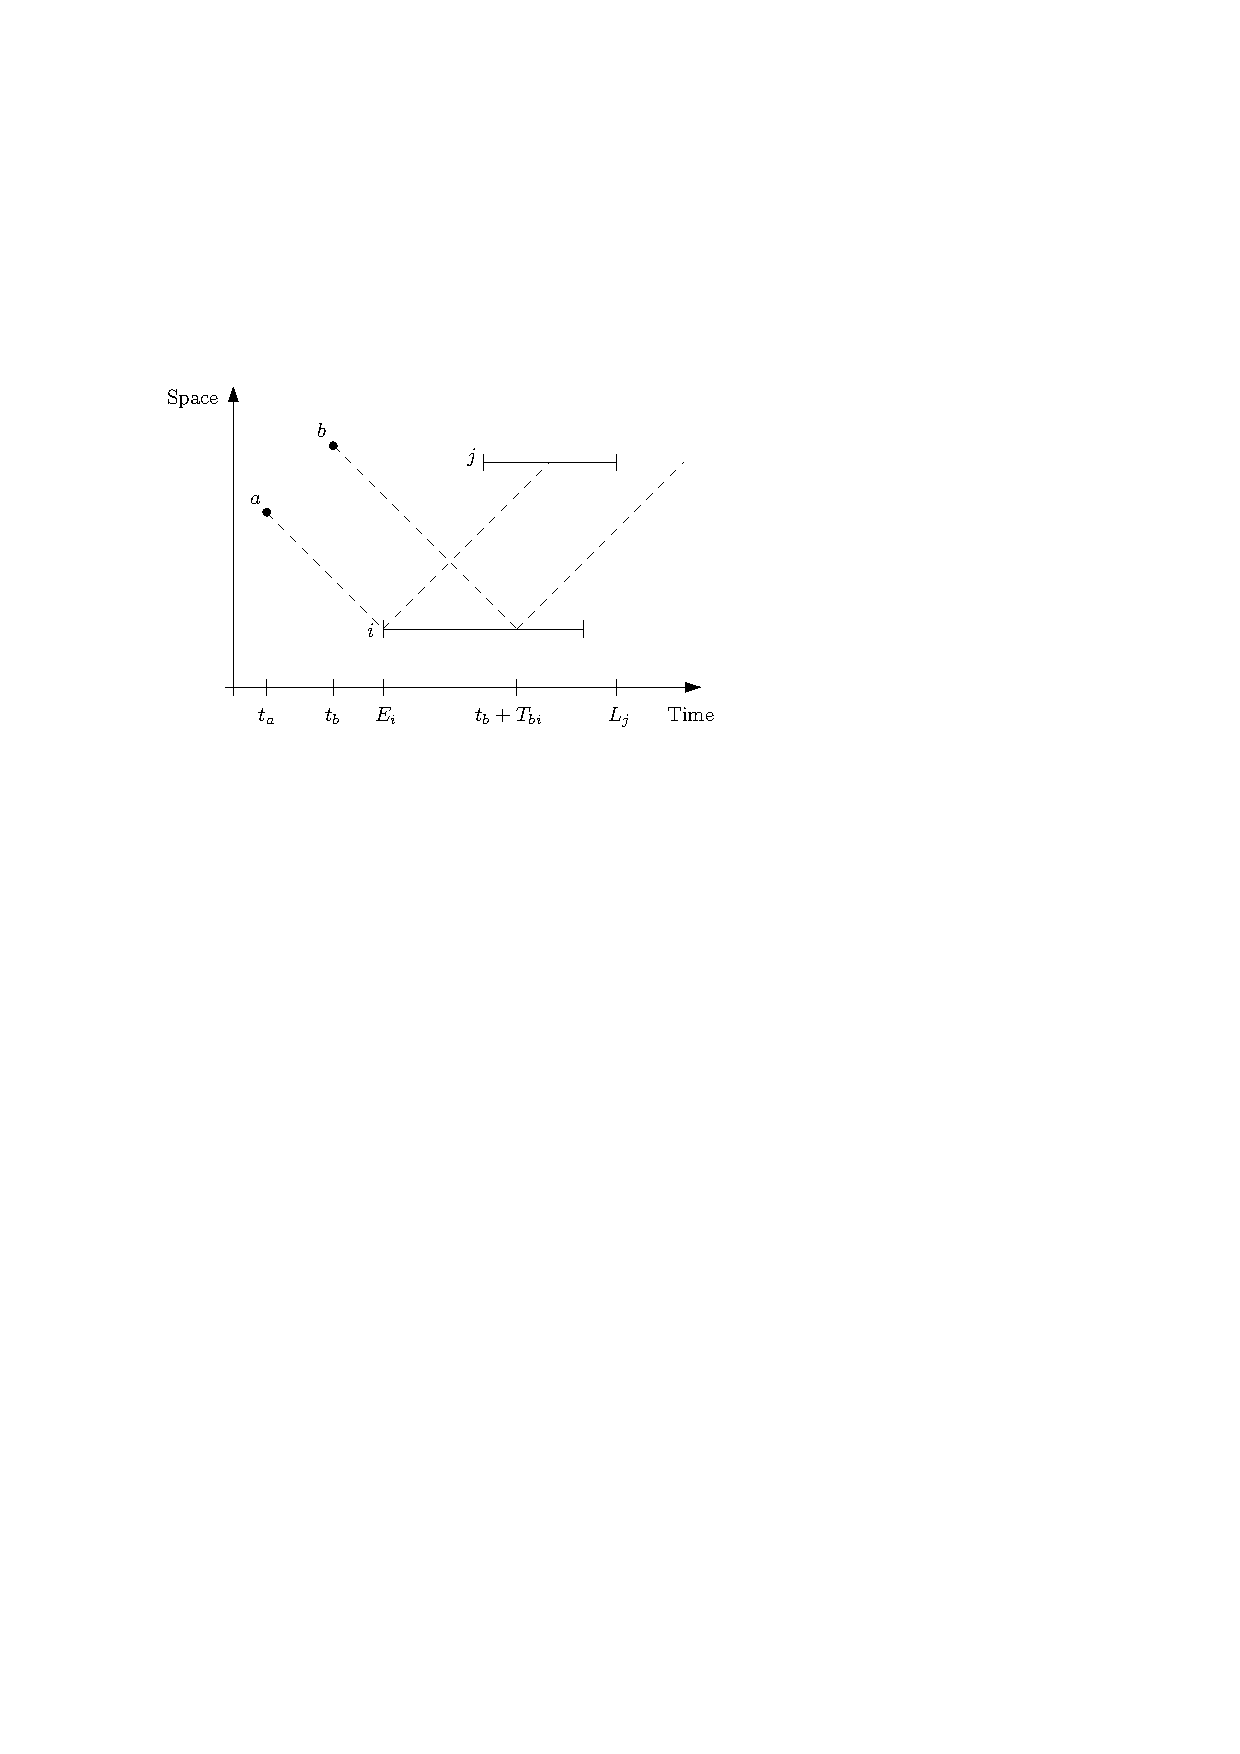
\includegraphics[width=0.9\columnwidth]{transitions01.pdf}
\caption{Feasible transitions. The figure shows the 
locations and time windows of two nodes $i$ and $j$.
If the vehicle left from $a$ at the instant $t_a$, visited node $i$
and moved directly to node $j$, the time constraint $L_j$ would be satisfied. 
However, assuming that at the instant $t_b$ the vehicle is located at $b$, the
transition $i \to j$ is seen to be infeasible.
}
\label{transitions01}
\end{center}
\end{figure}
The elements of the adjacency matrix are defined for all $i,j \in R_S$ by 
$L_{ij}= 1$, if $i \neq j$ and $i \to j$ is feasible, $L_{ij} = 0$ otherwise.

After the adjacency matrix $L$ has been determined, the hub vector $h=(h_1,\ldots,h_{|R_S|})$ of $L$ is determined by 
Equation \eqref{modhub} (here the remaining nodes $i \in R_S$ are numbered from $1$ to $|R_S|$ for clarity). 
A large hub score of node $i$ means that many 
nodes can be visited after $i$. 
The hub ranking method is defined as follows.
\begin{definition}[Hub ranking]
The remaining nodes $i \in R_S$ are sorted in descending order of the hub scores $h_i$: 
The branches are evaluated in the order $i_1,\ldots,i_{|R_S|}$, where
$h_{i_1} \geq h_{i_2} \geq \ldots \geq h_{i_{|R_S|}}$.
%branches beginning from good hubs
%are evaluated first.  
\end{definition}

% \textbf{Authority ranking:}
% The remaining nodes are sorted in ascending order of the authority scores; branches beginning from
% bad authorities are evaluated first.
The hub scores are used to give guidance to the algorithm regarding the order in which the 
depth-first search visits the nodes. 
Since the goal is to maximize the number of served customers, the sequences that can not improve the maximum 
number of served customers, can be discarded by studying the neighborhoods of the remaining nodes. 
\begin{definition}
 The neighborhood of node $i \in R_S$ is defined by $N(i) = \{i\} \cup \{j \in R_S \mid L_{ij} = 1\}$.
\end{definition}
\begin{theorem}
Let $S_{\max}$ denote the best found solution.
The sequence $S$ is suboptimal if 
\begin{align*}
C(S) + \max_{i \in R_S} C(N(i)) \leq C(S_{\max}),
\end{align*}
where $C(S), C(N(i))$ and $C(S_{\max})$ denote the number of drop-off points in $S,N(i)$ and $S_{\max}$,
respectively. 
\end{theorem}


\subsubsection{A heuristic extension}
\label{rrheuristic}
Algorithm \ref{rralg} describes an exact procedure for maximizing the number of served customers
in a single route. In order to find the exact solution, the algorithm goes through all
branches until no further nodes can be added to the current sequence or the sequence is seen to be suboptimal.

The effort of the algorithm can be controlled by limiting the number of branches that are evaluated
by means of a positive parameter $J$. For example, if $J=1$, the algorithm constructs a single sequence
and stops when the set of remaining nodes is empty. By increasing $J$ the search space is expanded and
if $J = (2n)!/2^n$ (the number of permutations that satisfy precedence constraints), the heuristic
coincides with the exact algorithm.


\subsubsection{Structure and complexity}
\label{rrstructure}
The structure of the ranking algorithm is as follows. 
Briefly described, each recursion step involves checking the the feasibility
of sequences $(S,i,j)$, where $i,j \in R_S$.
Clearly, this process has a complexity of order $\mathcal{O} (|R_S|^2)$,
where $|R_S|$ is the number of remaining nodes. 
After the adjacency matrix $L$ of the remaining nodes has been determined, the complexity of 
calculating $k$ steps of the power method (Equation \eqref{modhub}) is of order $\mathcal{O} (k |R_S|^2)$.

The overall complexity of finding a feasible solution is strongly dependent on the number of recursion
steps needed to find the solution. 
Finding a feasible solution to a problem with $n$ customers involves at least $2n$
recursion steps: At first, the number of remaining nodes is $2n$ and each time 
a feasible node is added to the end of the service sequence, the 
number of remaining nodes is decreased by one.
In the best case, no infeasible states are encountered and thus there are $2n$ recursion steps 
(one for each node added to the sequence).
At step $k \in \{1,\ldots,2n\}$, the number of remaining nodes is $2n+1-k$
and thus the complexity is of order $\mathcal{O} (\sum_{k=1}^{2n} (2n+1-k)^2) =\mathcal{O}(n^3)$.
Roughly, the computational work is linearly increased with the 
number of dead ends $M$ encountered during the recursion.
The overall complexity of the single vehicle algorithm is thus $\mathcal{O}(Mn^3)$.


\subsection{Numerical experiments}
\label{svexperience}
The following paragraphs present a summary of the computational results reported in \ref{jeadarp}. 
The exact and heuristic versions of the single-vehicle algorithm
were tested on a set of problems involving different numbers of customers and different time
window widths determined by a travel time ratio $R$ describing the maximum allowed ratio of travel time
to direct ride time. The pick-up and drop-off points of customers were chosen randomly from a
square-shaped service area and the ride times between the points were modeled by euclidean distances.

At first, the complexity of the problem was studied with respect to three parameters, namely
i) the number of customers $N$, ii) travel time ratio $R$ and iii) the average time interval $\mu$
between customer requests. The complexity of the exact algorithm was measured in terms of the
average number of feasible sequences
in \emph{feasible problem instances}, that is, randomized
problems for which at least one feasible solution was found. 
The number of feasible sequences gives us an insight on the complexity of the problem itself,
since any enumeration algorithm would have to evaluate the same number of feasible sequences.

Then, the performance of the heuristic with different objective functions was evaluated.
The complexity was measured in terms of the number of sequences evaluated by the heuristic.

The experiments were performed on a standard laptop computer with a 2.2 GHz processor. 
The CPU times and the number of evaluated sequences appeared to have a roughly linear relationship.
A typical problem instance involving 20 customers could be solved up to optimality within less than a second.

\begin{figure}[ht]
\begin{center}
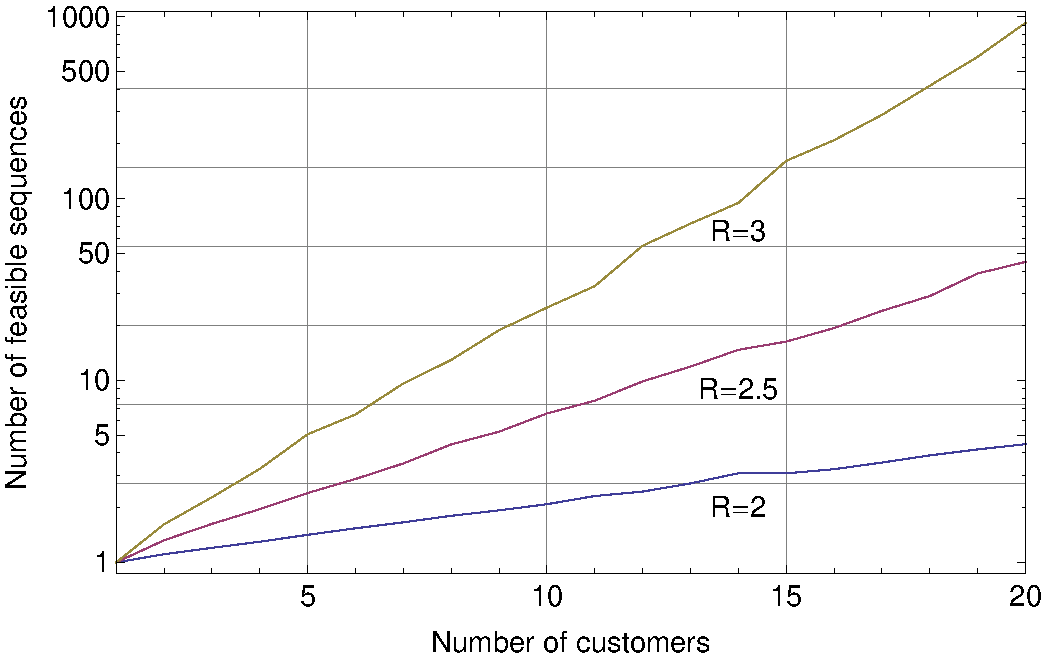
\includegraphics[width=0.9\textwidth]{nvertailu01.pdf}
\caption{Experiment 1. The complexity of the exact algorithm with respect to the number of customers on a logarithmic scale. 
The three curves represent, as a function of the number of customers, the average number of feasible sequences 
for $R=2,2.5,3$ and $\mu=1800$s. Clearly, the complexity increases exponentially with respect
to the number of customers.}
\label{nvertailu01}
\end{center}
\end{figure}



\begin{figure}[ht]
\begin{center}
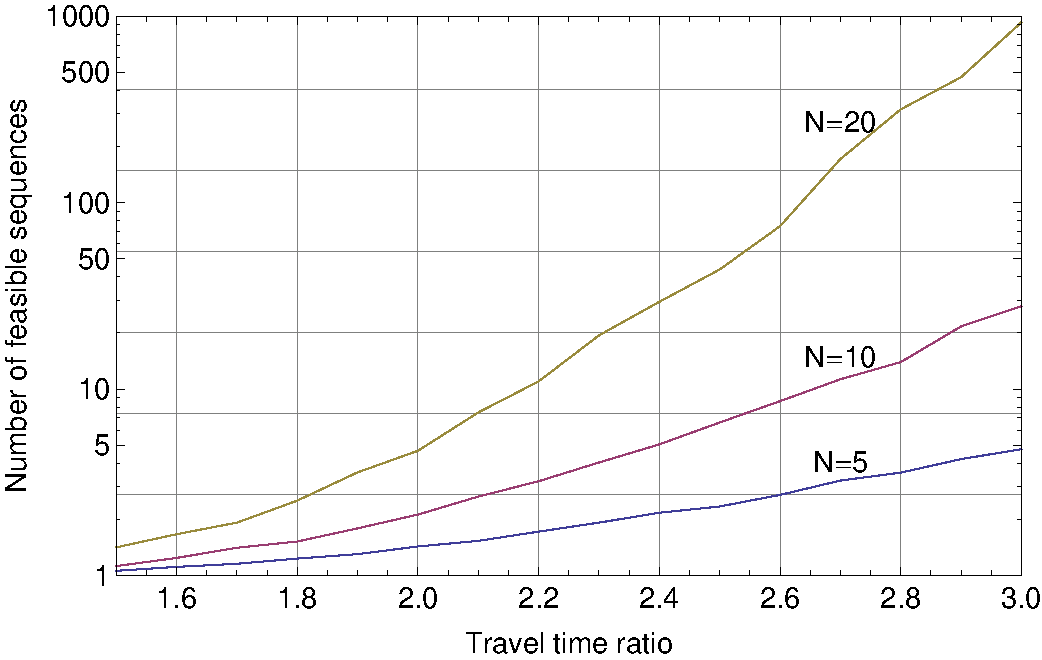
\includegraphics[width=0.9\textwidth]{ttivertailu01.pdf}
\caption{Experiment 2. The complexity of the exact algorithm with respect to travel time ratio on a logarithmic scale. 
The three curves represent, as a function of the travel time ratio, the average number of feasible sequences
for $N=5,10,20$ and $\mu = 1800$s.}
\label{ttivertailu01}
\end{center}
\end{figure}


\begin{figure}[ht]
\begin{center}
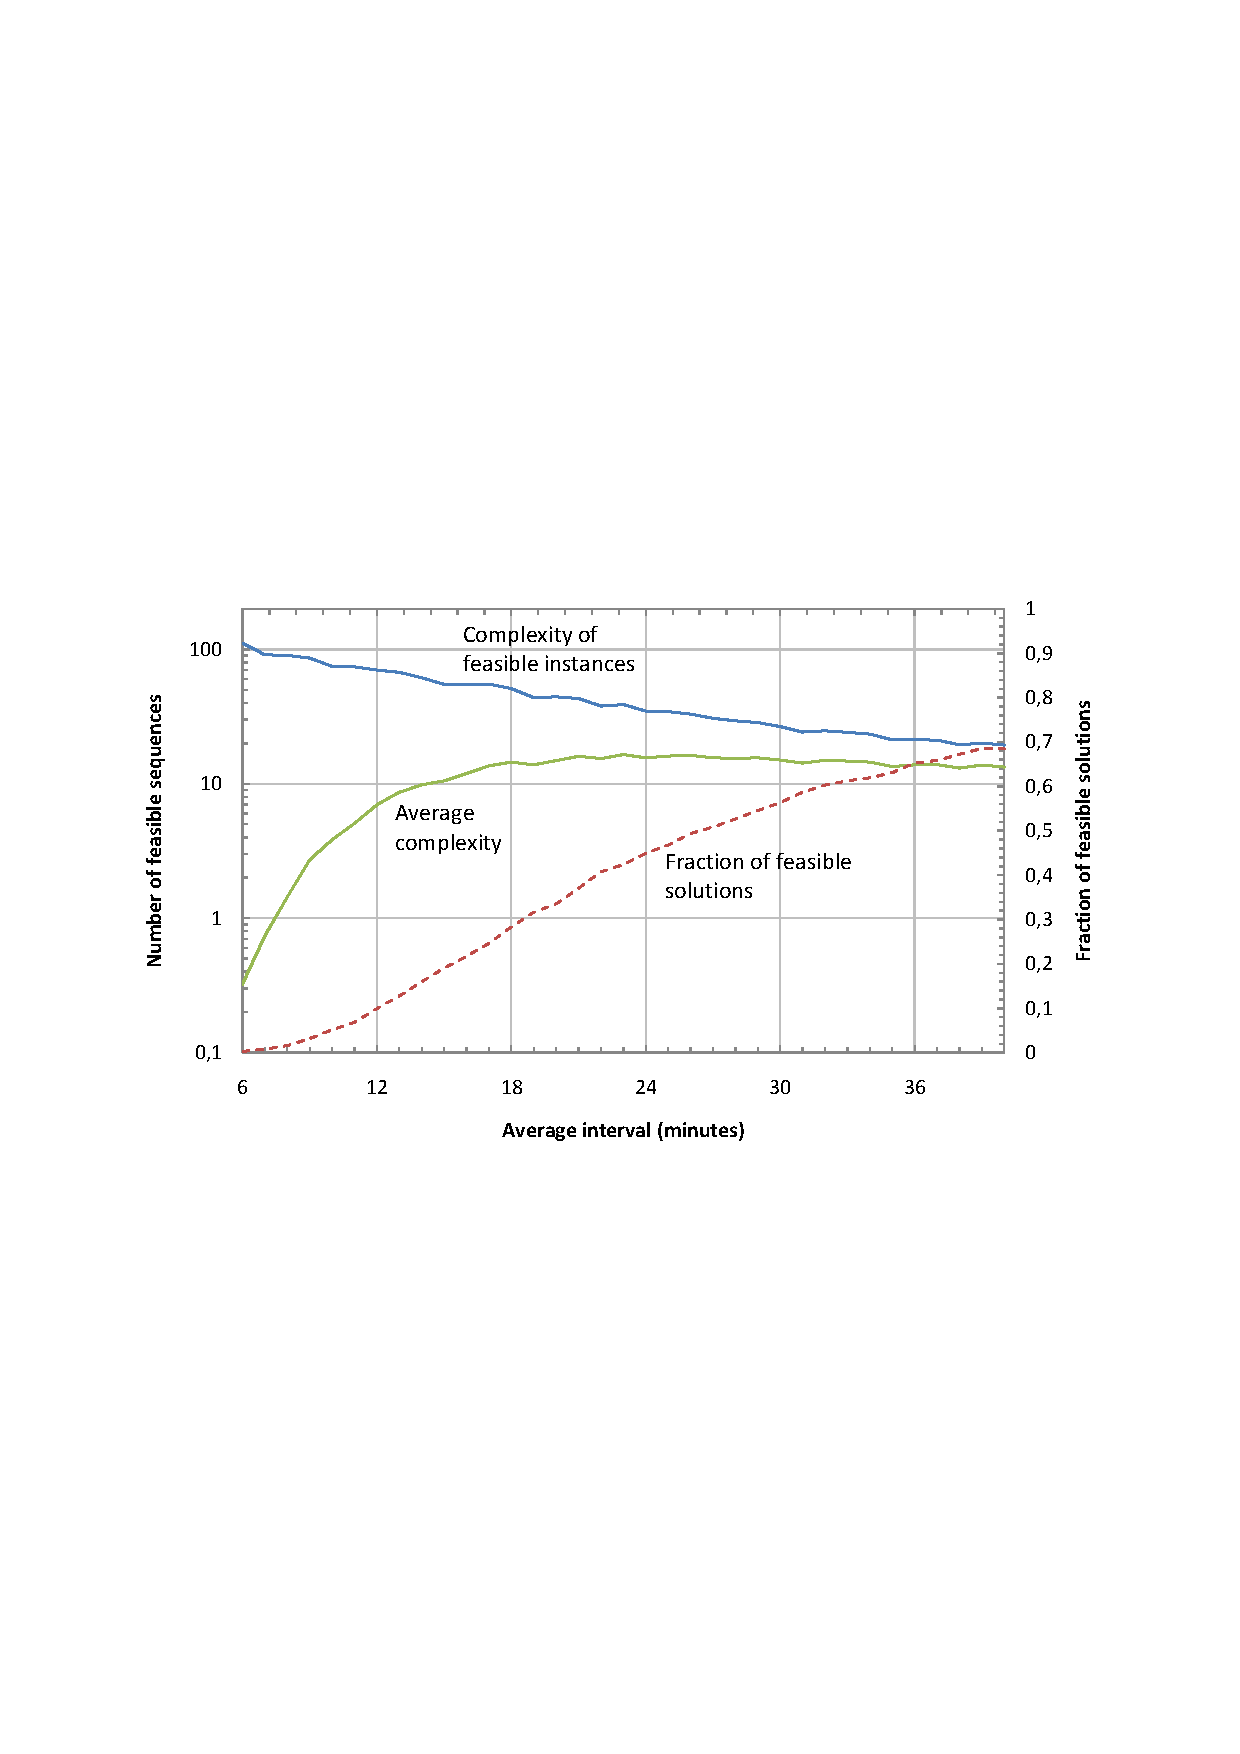
\includegraphics[width=1.0\textwidth]{intvertailu01.pdf}
\caption{Experiment 3. The complexity of the exact algorithm with respect to the average time 
interval between customers. The solid lines represent the average number of feasible sequences in
feasible problem instances and all problem instances, on a logarithmic scale for $N=10$ and $R=3$.
The dashed line corresponds to the fraction
of problem instances, for which at least one feasible solution was found.}
\label{intvertailu01}
\end{center}
\end{figure}


\begin{figure}[ht]
\begin{center}
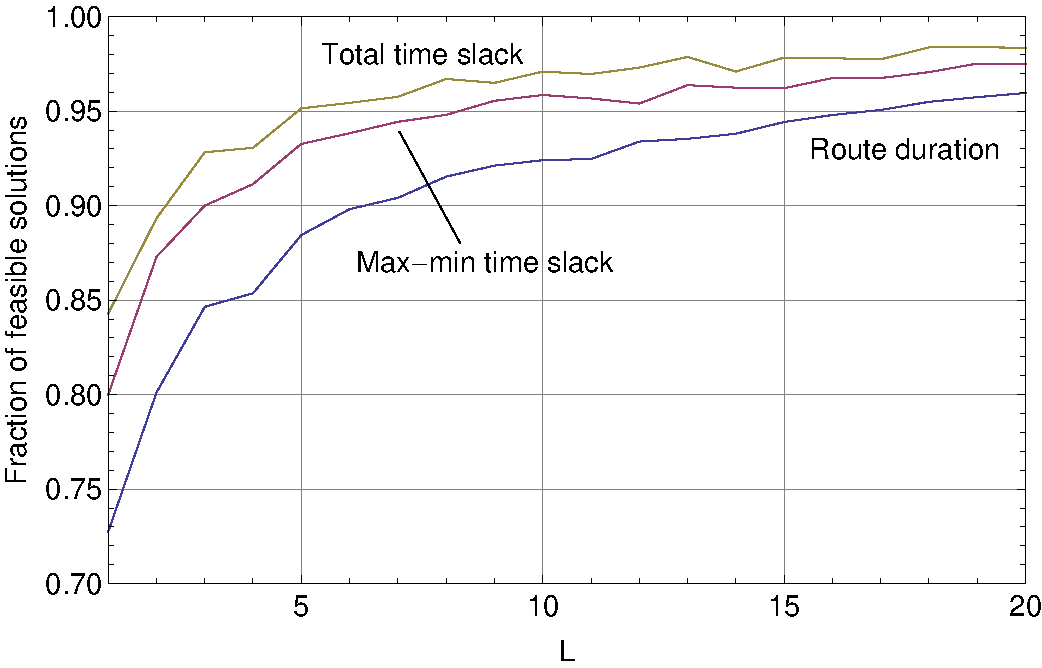
\includegraphics[width=0.9\textwidth]{objvertailu01.pdf}
\caption{Experiment 4. The performance of three different heuristic objective functions as functions of degree $L$.
The curves represent the fractions of instances for which a feasible solution was found by the objective functions 
(compared to the exact algorithm), 
for $N=20$, $R=3$ and $\mu=1800$s. The total slack time objective function
outperforms the other two in all studied cases.
}
\label{objvertailu01}
\end{center}
\end{figure}




\subsubsection{Experiment 1: Number of customers}
%At first we study the complexity of the exact algorithm with respect to the number of customers.
In practice, the number of customers assigned to a single vehicle is governed by the
pre-order time of the dial-a-ride service: If customers may request service in
advance, the planned vehicle routes are expected to be longer than in immediate-request
services. Figure \ref{nvertailu01} shows the average number of feasible sequences in feasible problem instances 
on a logarithmic scale, computed over 10000
randomized instances for $N=1\ldots 20$, $R = 2,2.5,3$ and $\mu = 1800$s.

Referring to the figure, it can be seen that the complexity of the problem increases exponentially
with respect to the number of customers with all studied values of the travel time ratio.  
In addition, the complexity is increased with the travel time ratio. 

\subsubsection{Experiment 2: Travel time ratio}
%Let us study the complexity of the exact algorithm as a function of travel time ratio.
Figure \ref{ttivertailu01} shows the average number of feasible sequences in feasible problem instances 
on a logarithmic scale, computed over 10000
randomized instances for $R=1.5\ldots 3$, $N = 5,10,20$ and $\mu = 1800$s. 


The figure shows that the effect of the travel time ratio on the complexity of the problem is significant.
The fact that the slopes of the curves increase with $R$ on the logarithmic scale indicates that the relation 
between complexity and $R$ is superexponential.


\subsubsection{Experiment 3: Time interval}
%Let us conclude the study of the exact algorithm by examining complexity with respect to the average time interval between customer requests. 
The solid lines in Figure \ref{intvertailu01} represent the average number of feasible sequences in
(i) feasible problem instances and (ii) all problem instances, on a logarithmic scale, computed over 10000
randomized instances for $N=10$, $R=3$ and $\mu = 6 \ldots 40$ minutes. The dashed line corresponds to the fraction
of problem instances, for which at least one feasible solution was found.

The figure indicates that the complexity of feasible problem instances decreases exponentially 
with respect to the average time interval $\mu$. On the other hand, the probability of finding
at least one feasible solution is increased with $\mu$. By looking at the curve corresponding 
to the average complexity of all problem instances (including infeasible cases), it can be seen that the
complexity is maximized at a certain time interval ($\mu = 24$ minutes in this case), in which both the probability of
finding a feasible solution and the number of feasible sequences in feasible cases are relatively large.

At this point, it should be emphasized that the above results apply to randomized instances for the 
single vehicle problem. In a dynamic multiple vehicle setting, an effort is made to 
divide the customers among available vehicles optimally. Thus, it is suggested that a larger number of customers
can be served by a single vehicle in less time than in the case in which the customers' pick-up
and drop-off locations are completely random. However, the above results give us an insight on
how the complexity of the single vehicle subroutine behaves with respect to the average time interval between
the earliest pick-up times of customers assigned to a single vehicle.


\subsubsection{Experiment 4: Objective functions}
Let us study the performance of the three different heuristic cost functions \eqref{rl}, \eqref{ts} and \eqref{maxmin}
as a function of the degree $L$ of the heuristic.
Figure \ref{objvertailu01} shows the fraction of problem instances for which a feasible solution was 
% in feasible problem instances obtained 
found by the heuristic (compared to the exact algorithm), computed over 10000
randomized instances. 
The number of customers was set to $N=20$, the travel time ratio
was $3$ and the average time interval $\mu = 1800$s was used.

Referring to the figure, it can be seen that the total time slack cost function \eqref{ts} is capable of finding
a feasible solution to randomized problems most often, while the performance of the route duration cost
function \eqref{rl} is worst of the three algorithms. Note that as the degree $L$ is increased, 
the fraction of feasible solutions converges to 1 for any heuristic cost function, since whenever $L \geq \frac{(2N)!}{2^N}$,
the heuristic coincides with the exact algorithm regardeless of the studied problem.



% 
% \subsection{Conclusions}
% In this work, an exact optimization procedure is developed to solve the
% static and dynamic versions of the single vehicle dial-a-ride problem with time 
% windows. Using complete enumeration to solve the problem with respect
% to a generalized objective function is motivated by the dynamic nature of 
% online demand responsive transport services,
% in which looking only at the tentative route duration, as in existing algorithms for the problem,
% may decrease the possibilities of serving future customers.
% 
% In addition, an adjustable heuristic extension to the algorithm
% is introduced, in order to be able to control the CPU times:
% If the problem size is reasonable, the proposed solution method
% produces globally optimal solutions. If the problem size is increased, 
% the algorithm adjusts itself to produce locally optimal solutions,
% closing the gap between the classical insertion heuristic and the exact solution and thus
% making the algorithm applicable to any static or dynamic dial-a-ride problem.
% 


\section{Multi-vehicle dial-a-ride problem}
\label{multivehicle}
Most recent studies related to the dial-a-ride problem are related to the multi-vehicle case, in which 
a set of vehicle routes is designed for a predefined set of customers, see for example 
\cite{cordeau02, cordeau01, bent, ropke, xiang2006, melachrinoudis, parragh, garaix, berbegliathesis,berbegliafeas,berbegliapdp}.
Reference \cite{berbegliafeas} examines the multi-vehicle dial-a-ride problem as a \emph{constraint satisfaction problem}, in which the goal
is to find a set of $m$ feasible vehicle routes that serve all customers, where $m$ is the 
number of vehicles, or to prove that such a set of routes does not exist.
In this reference, it is noted that 
an algorithm for checking the feasibility of a DARP instance has two main applications:  
1) Determining the feasibility can be the first phase in an 
optimization algorithm in a \emph{static} setting, where all trip requests are known, for example, one day in advance. 
2) In \emph{dynamic} services, a constraint satisfaction algorithm can be used 
for deciding whether to accept or reject incoming user requests. 

This work is partly motivated by the latter application, namely, a dynamic demand-responsive transport (DRT) service 
currently being planned to operate in Helsinki. The service, run by 
Helsinki Region Transport, The Finnish Transport Agency and Aalto University,
will be deployed by the end of 2012.
Similarly as the current service routes \cite{jouko}, the new DRT
service is designed to operate on a demand-responsive basis, that is, 
each trip is booked in advance and the vehicle routes are modified according to
the trips. The main difference to existing services is 
that no pre-order times for trips are required and the trips can be booked
"on the fly" by means of an interactive user interface. 
A main goal is to provide high-quality service that could compete with
private car traffic. 

In addition to passenger transportation, we note that a time-constrained problem similar to the DARP arises in 
food delivery services. Instead of passengers with pick-up and drop-off time windows, the goal is to transport 
\emph{meals} from restaurants to specified delivery points within guaranteed time limits.
Similarly as in the dynamic DARP, the food delivery service provider needs to decide quickly whether to take an incoming order or not,
if there is a guaranteed maximum delivery time, for example, one hour.

In both contexts (passenger transportation and food service), a good level of service means that the problem is highly constrained \cite{jokinen-fists-2011}. 
In such problems, the number of feasible solutions becomes so limited that often
any feasible solution will be relatively close to the optimal solution with respect to the
objective function \cite{psaraftis02}.
Thus, we suggest that in highly constrained cases, solving the consraint satisfaction problem provides, 
if not the optimal solution, at least a good initial solution. 

The main result of \ref{jhitsdarpts} is an exact algorithm for the constraint satisfaction dial-a-ride problem
introduced in \cite{berbegliafeas}. In contrast to most works related to vehicle routing and dial-a-ride problems,
no specific cost function is considered\footnote{
For approaches to vehicle routing and dial-a-ride problems with cost functions, 
we refer to \cite{braysy01,braysy02,groer} and \cite{cordeau02,berbegliahybrid}.}. 
The algorithm stops as soon as a feasible solution is found regardeless of
the quality of the solution. If a feasible solution is not found through exhaustive search, the algorithm 
proves that the problem instance is infeasible. In addition, some infeasible instances are detected in advance
by studying the feasiblility of routes involving two customers. 



\subsection{The maximum cluster algorithm [\ref{jhitsdarpts}]}
\label{mvsolution}
\ref{jhitsdarpts} presents the following exact approach to the multi-vehicle DARP as a constraint satisfaction problem.
By using the ranking algorithm (Algortithm \ref{rralg}) described in Section \ref{routingbyranking} as a subroutine,
 the method produces a feasible solution to 
any instance or proves that the instance is infeasible. The main idea is that the vehicle routes are constructed
one by one, each maximizing the number of served customers in the set of remaining customers.
The customers are denoted by numbers $1,\ldots,n$ and the vehicles are denoted by numbers $1,\ldots,m$.

First, a route is constructed for vehicle $1$, serving as many 
customers as possible. Then, the process is repeated with vehicle $2$ for the set of customers
that were not served by vehicle $1$ and so forth (see Figure \ref{greedyidea}). 
Letting $X$ denote a
set of customers, we denote by RR($X$) the single-vehicle ranking algorithm (Algorithm \ref{rralg}) that returns a route 
that maximizes number of served customers in set $X$ and the corresponding set of served customers.
This set will be referred to as a maximum cluster of $X$, which is formally defined as follows.
\begin{definition}
Let $X$ be a set of customers and $M \subset X$ be a subset of $X$, for which there exists a feasible 
route serving all customers in $M$. If $|M| \geq |Y|$ for all sets $Y \subset X$
for which there exists a feasible route serving all customers in $Y$, then $M$ is a \emph{maximum cluster} of $X$.
\end{definition}
Note that if there exists a feasible route serving all customers in $X$, we have $M(X) = X$.
The solution to the multi-vehicle case is outlined in Algorithm \ref{alg03}.

\begin{algorithm}
\begin{algorithmic}
\FORALL {$k \in \{1,\ldots,m\}$}
\STATE \ \ $[S_k,X_k'] \leftarrow $ RR($X_k$); \hfill ($S_k$ = route, $X_k'$ = set of served customers)
\STATE \ \ $X_{k+1}  \leftarrow X_{k+1} \cup (X_k \setminus X_k')$, where $X_{m+1} = X_1$;
\ENDFOR
\end{algorithmic}
\caption{Outline of the multi-vehicle algorithm. $X_k$ denotes the set of customers assigned 
to vehicle $k$ and RR($X_k$) denotes the single-vehicle 
subroutine presented in Algorithm \ref{rralg} that returns
a maximum cluster $X_k'$ of $X_k$ and the corresponding route $S_k$. 
Initially, all customers are assigned to the first vehicle, that is, $X_1 = \{1,\ldots,n\}$ and $X_k = \emptyset$ for all $k \in \{2,\ldots,m\}$.}
\label{alg03}
\end{algorithm}


\begin{figure}[ht]
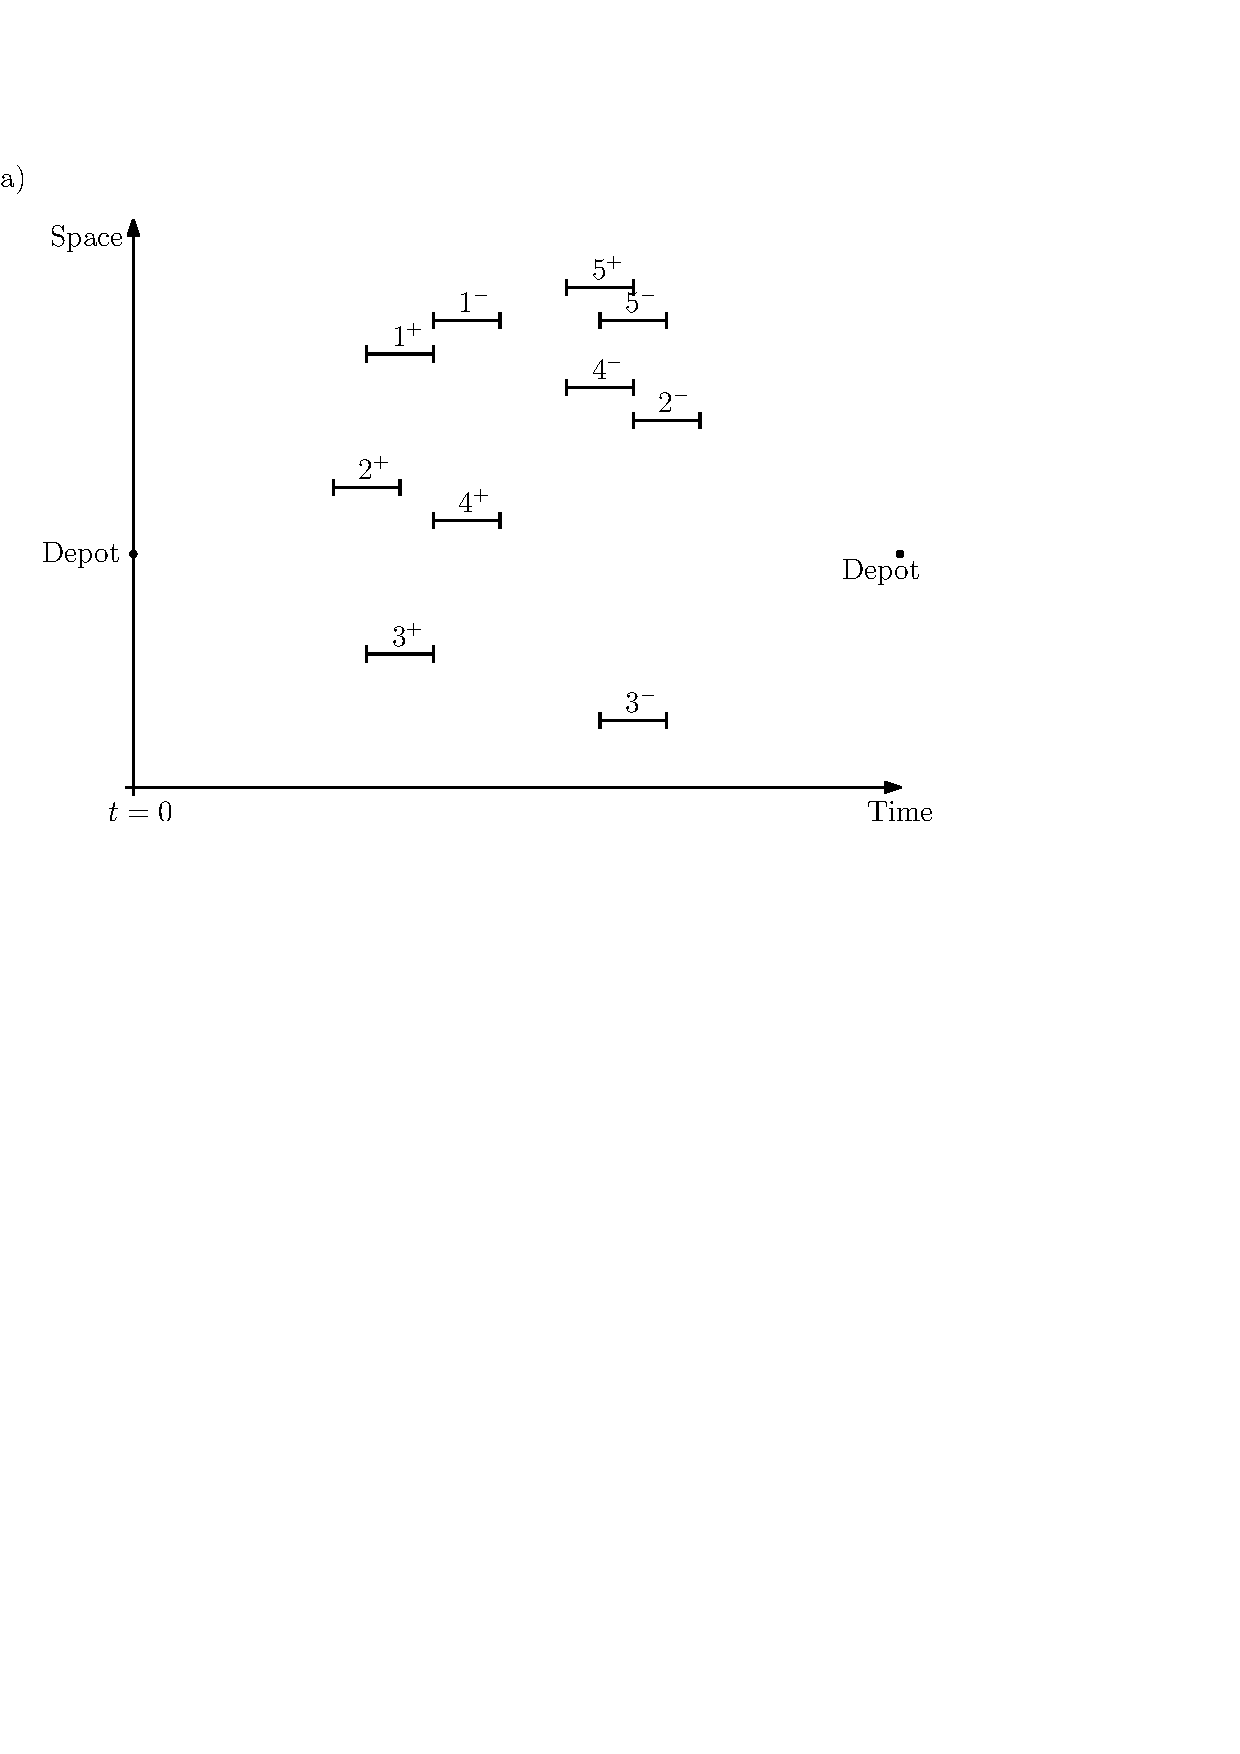
\includegraphics[width=0.45\textwidth]{greedy01b.pdf} \ \ \ \ \  \ \ \ \ \  
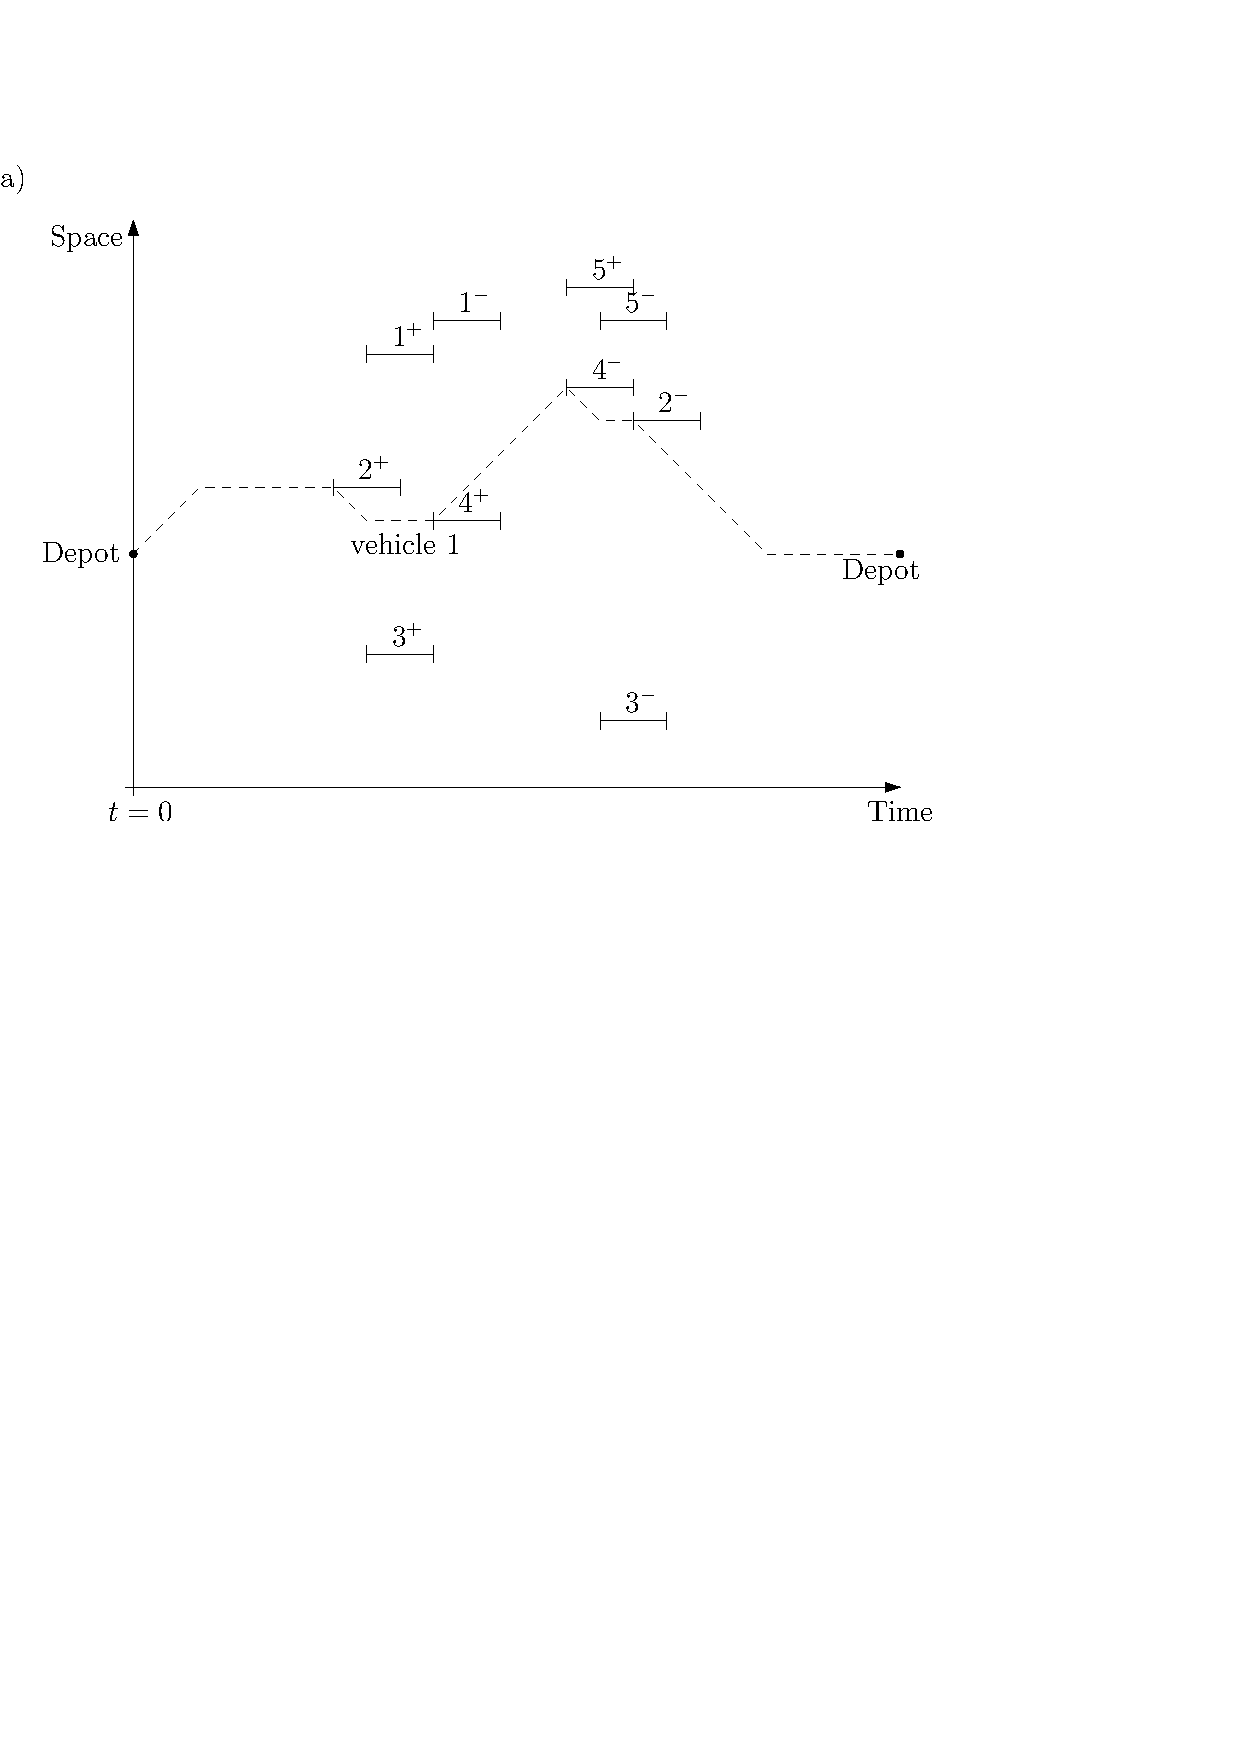
\includegraphics[width=0.45\textwidth]{greedy05b.pdf}  \\ \ \\  
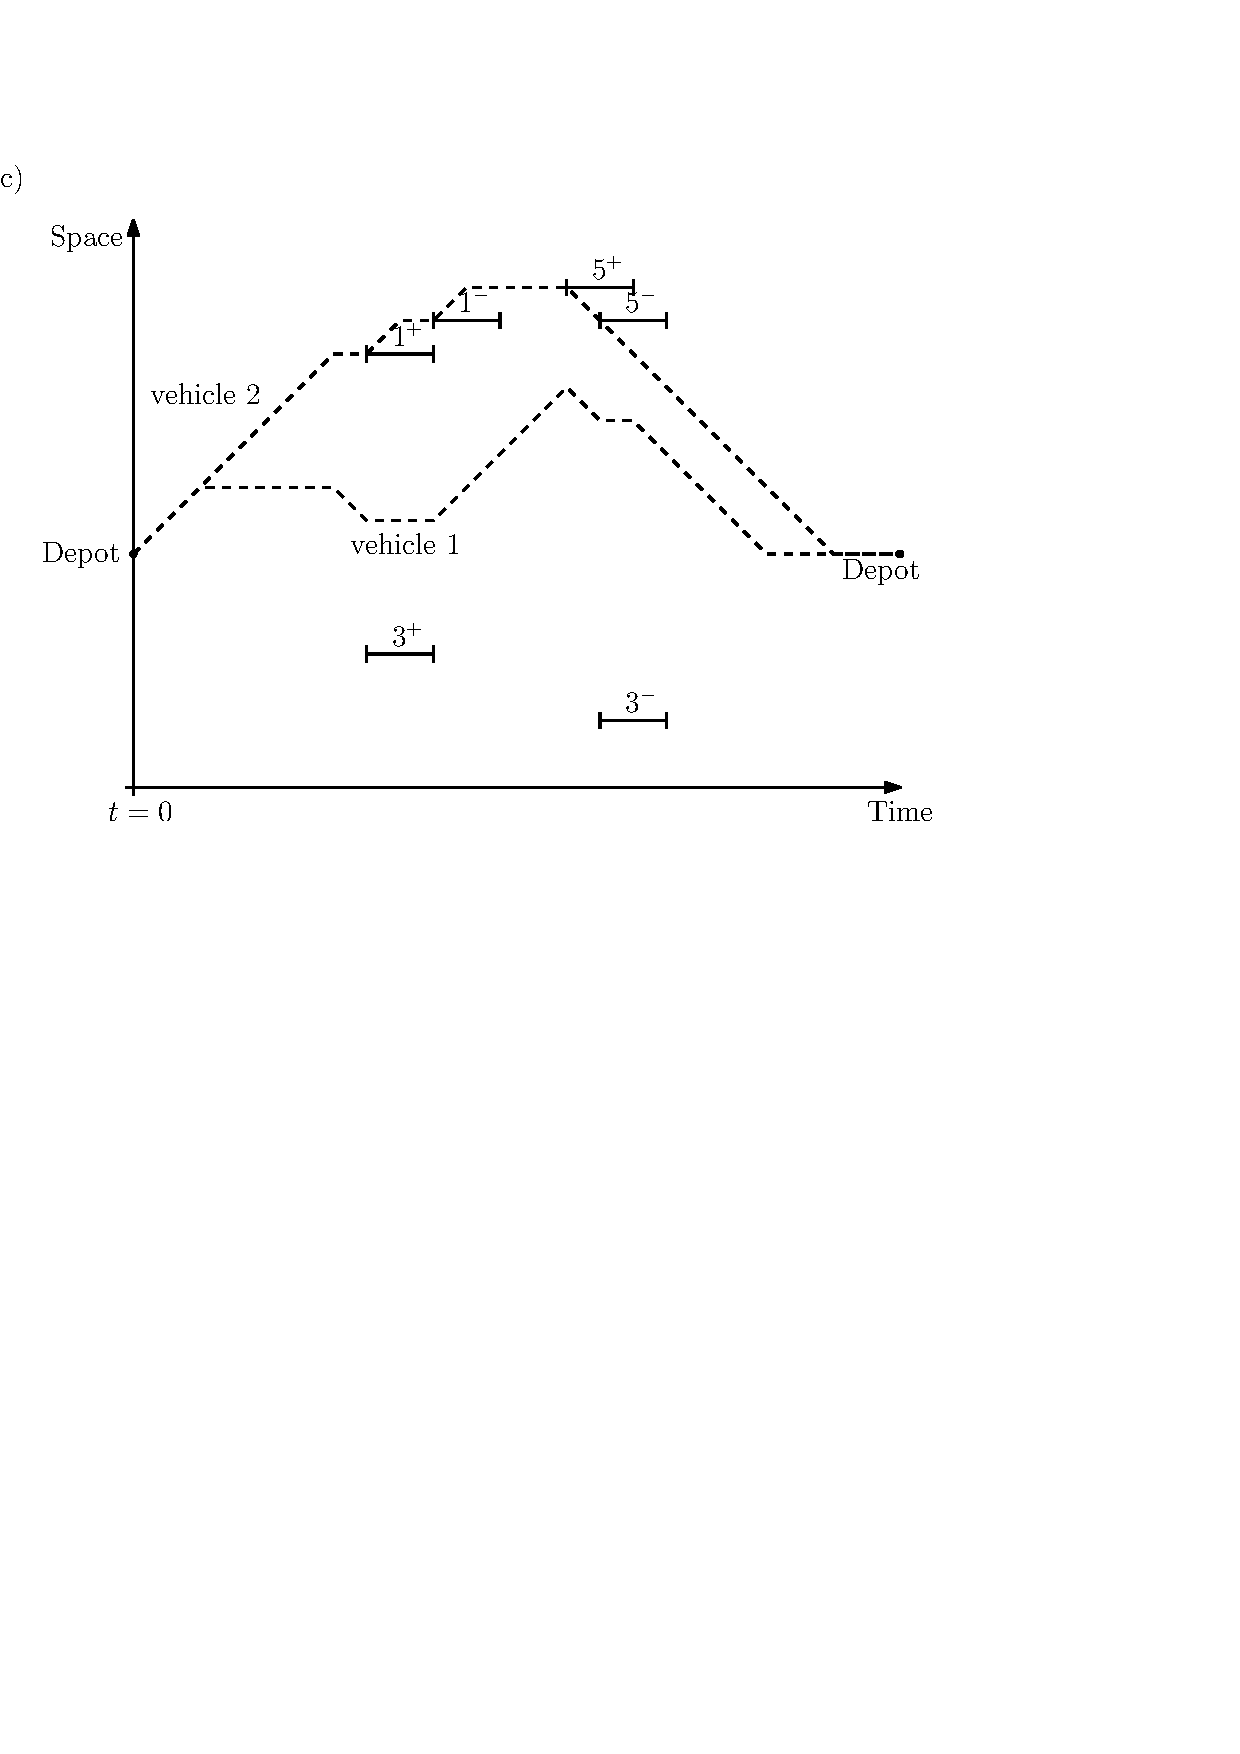
\includegraphics[width=0.45\textwidth]{greedy06b.pdf} \ \ \ \ \  \ \ \ \ \   
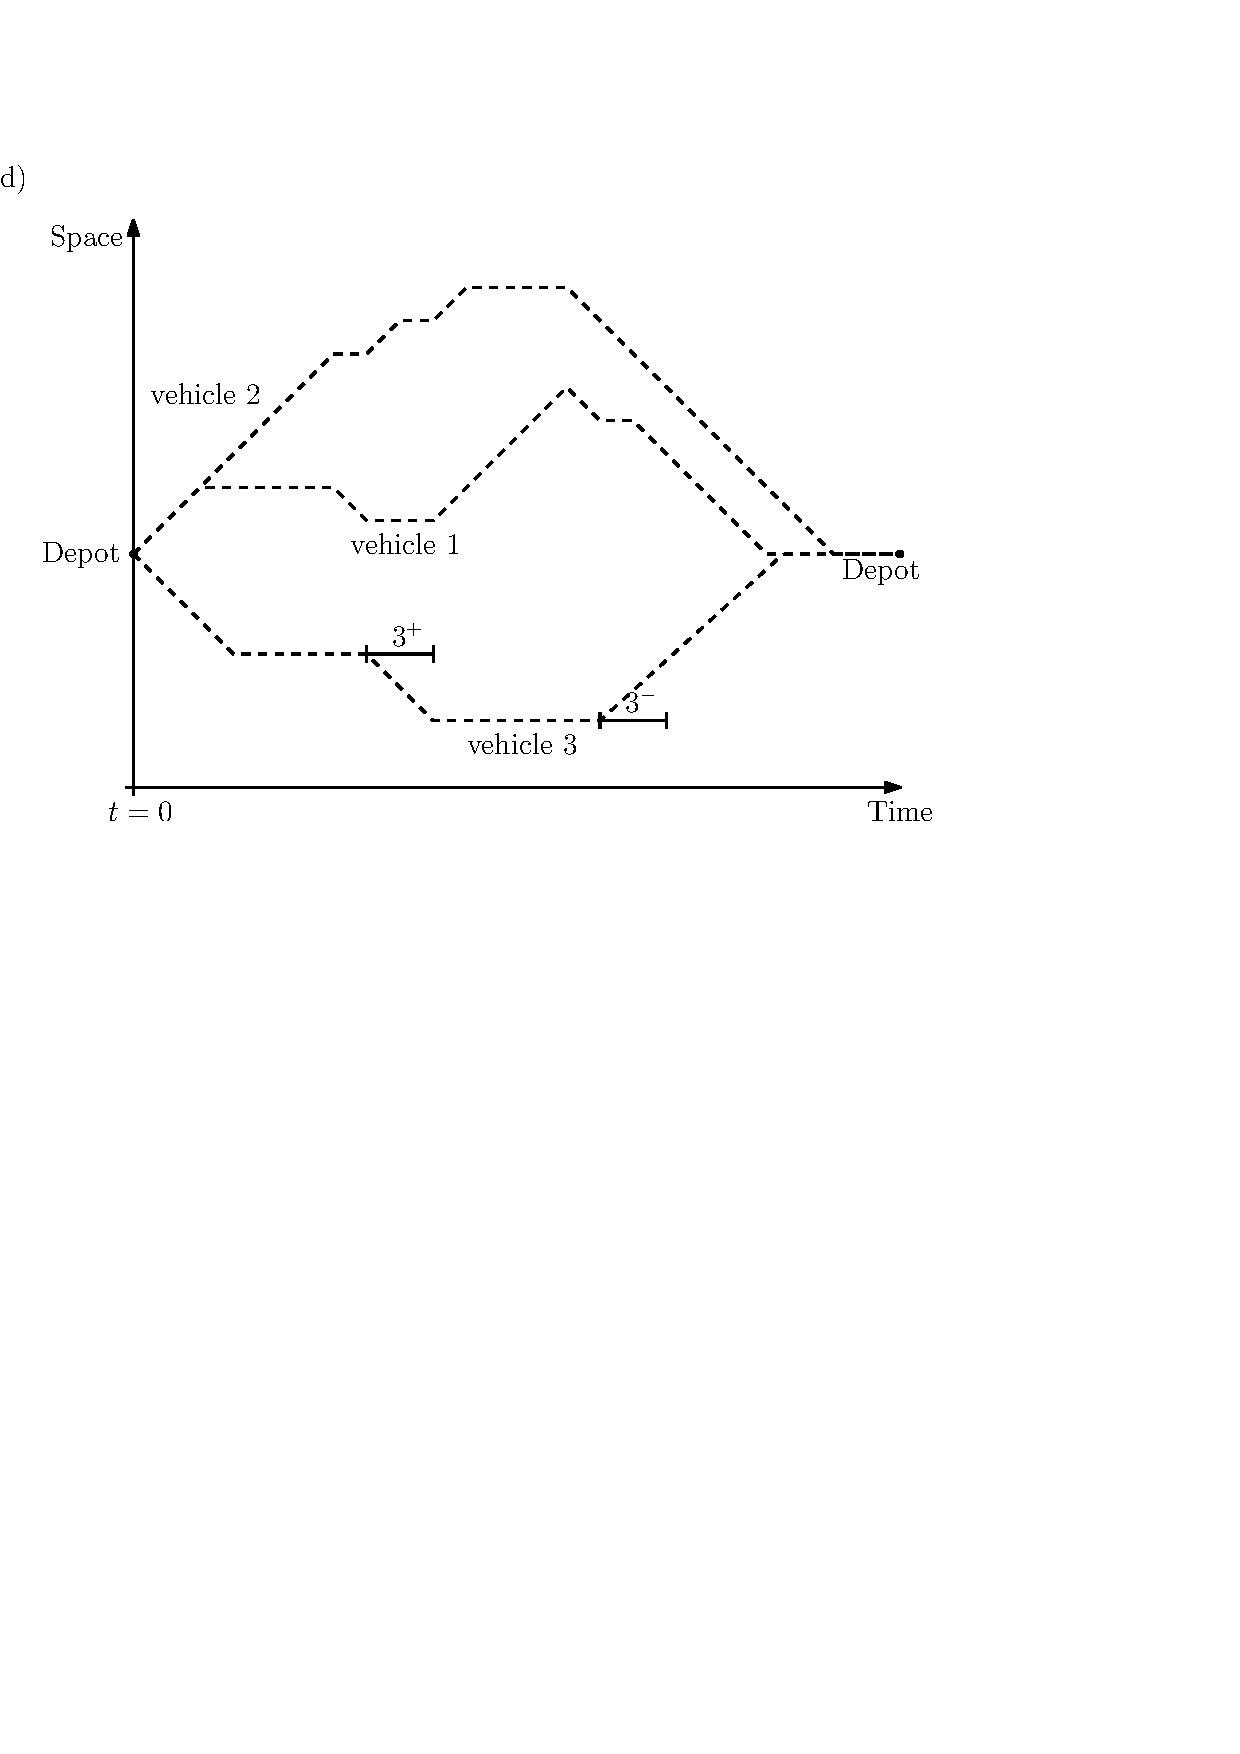
\includegraphics[width=0.45\textwidth]{greedy07b.pdf}  \\ \ \\   
\caption{A one-dimensional example of the approach to the multi-vehicle problem involving five customers 
and three vehicles. The first route is constructed by maximizing 
the number of customers that can be served by a single vehicle (Figure b). 
Then, the customers $2$ and $4$ served by the first vehicle are removed from the set of remaining customers and the process 
is repeated for the second vehicle (Figure c). Finally, a route is construced for the third vehicle, serving the
last remaining customer $3$ (Figure d).
}
\label{greedyidea}
\end{figure}

\subsection{Iteration}
\label{iteration}
If a feasible solution is not found directly by using the procedure described in Algorithm \ref{alg03}, 
the process is repeated. The goal is to find a set of customer-vehicle assignments 
such that for each vehicle there exists a feasible route serving all customers assigned to the vehicle
or to prove infeasibility by going through all possible sets of customer-vehicle assignments.

Formally, we define a \emph{partition} of customers as a disjoint cover of $\{1,\ldots,n\}$ consisting of $m$ sets $(X_1,\ldots,X_m)$,
where $X_k$ denotes the set of customers assigned to vehicle $k$.
The set of all partitions is denoted by $\mathcal{P}$. Since each customer can be assigned to any of the $m$ vehicles, the total 
number of possible partitions is equal to the Stirling number of the second kind, that is,
$|\mathcal{P}| = S_2(n,m) = \frac {1}{m!} \sum_{i=0}^{m} (-1)^i {m \choose i} (m-i)^n$.
A partition is said to be \emph{feasible}, if $M(X_k) = X_k$ for all $k \in \{1,\ldots,m\}$.

Note that if the multi-vehicle instance has a solution,
there exists a partition $(X_1^*, X_2^*, \ldots, X_m^*)$ for which $M(X_k^*)=X_k^*$ for all $k \in \{1,\ldots,m\}$. 
Thus, infeasibility can be proved by iteratively checking all partitions for feasibility.

%The main idea in going through all partitions is that 
Each iteration starts with the \emph{candidate} partition $(X_1,\ldots,X_m)$ and 
results in another partition $(X_1',\ldots,X_m')$. If the partition $(X_1',\ldots,X_m')$ is not feasible,
the candidate partition $(X_1,\ldots,X_m)$ is marked as 'checked'. Otherwise, a feasible solution 
has been found and the algorithm is terminated.

If $(X_1',\ldots,X_m')$ is marked as 'checked', the algorithm proceeds to the next candidate partition that is
not marked as 'checked'.
Otherwise, $(X_1',\ldots,X_m')$ becomes the
candidate partition, $(X_1,\ldots,X_m) \leftarrow (X_1',\ldots,X_m')$. 

The main idea is that the first iteration (Algorithm \ref{alg03}) produces an \emph{initial candidate partition} of customers, 
which is improved during later iterations. This procedure is motivated by the fact that the initial vehicle routes are
constructed by attempting to serve as many customers as possible from the initial set 
$\{1,\ldots,n\}$ of all customers. After the initial routes have been determined, 
we know that at least the 
customers in $X_k'$ can be served by vehicle $k$. Thus, for any set $X$, the number of 
served customers from the set $X \cup X_k'$ is \emph{at least} equal to the number of customers
in the set $X_k'$. A customer $x$ that has relatively few feasible transitions to all nodes may 
be in a good position with respect to the customers assigned to a
single vehicle $k$. That is, even if customer $x$ was left out of the initial 
vehicle routes due to a small number of feasible transitions to other nodes,
$x$ can be added to one of the routes during a later iteration. 


\subsection{A priori screening}
\label{earlydetection}
Since the  
number of possible partitions of $n$ customers into $m$ sets is equal to the Stirling number of the second kind,
going through all possible partitions is computationally taxing.
However, some instances 
are rendered infeasible by studying the feasibility of routes involving two customers as follows: 
If there exist no feasible
routes involving customers $\{i,j\}$, an arc between $i$ and $j$ is formed. This means that 
customers $i$ and $j$ can not be assigned to the same vehicle. Then, the \emph{maximum clique} $C$
is determined, that is, the largest set of customers for which there is
an arc between all pairs of nodes $i,j \in C$, see \citep{wood1997}. If the size of the maximum clique
is greater than the number $m$ of vehicles, the instance is infeasible since there are $|C| > m$ customers
which should all be served by different vehicles. 

Otherwise, since the customers in the maximum clique $C = \{c_1,\ldots,c_{|C|}\}$ all have to be assigned to different vehicles, 
with no loss of generality we may initially assign customer $c_j$ to vehicle $j$ for all $j \in \{1,\ldots,|C|\}$.
Then, the set of \emph{feasible vehicles} $V_i$ for each customer $i$ is determined by noting that if there is an 
arc between $i$ and $c_j \in C$, customer $i$ may not be assigned to the same vehicle as $c_j$.

After the set of feasible vehicles $V_i$ has been determined for each customer $i \in \{1,\ldots,n\}$,
the set of \emph{a priori feasible partitions} is defined as follows.
\begin{definition}
A partition $(X_1,\ldots,X_m)$ of customers is feasible a priori, if $i \in X_k \Rightarrow k \in V_i$ for all $k \in \{1,\ldots,m\}$.
The set of a priori feasible partitions is denoted by $\mathcal{P}'$.
\end{definition}
Note that assigning each customer $i$ a vehicle number $v_i \in V_i$ defines a unique partition.
Since the vehicle number of customer $i$ can be chosen from the set $V_i$ of feasible vehicles, 
the number of a priori feasible partitions is given by $|\mathcal{P}'| = \prod_{i=1}^n |V_i|$.

\begin{theorem}
\label{partitions}
The number of a priori feasible partitions satisfies $|\mathcal{P}'| \leq m^{n-|C|}$.
\end{theorem}

The set of a priori feasible partitions is represented by the set $V_1 \times \ldots \times V_n$ and each a 
priori feasible partition is represented by a vector $(v_1,\ldots,v_n) \in V_1 \times \ldots \times V_n$.
Information on checked partitions is stored in a sparse array 'CHECKED'.
The partitions not marked as checked are included in the set of remaining partitions $I$
(initially $I = V_1 \times \ldots \times V_n$).
During run-time, each candidate partition is marked as 'checked' by setting CHECKED$(v_1,\ldots,v_n) = 1$ and
removed from the set of remaining partitions, that is, $I \leftarrow I \setminus \{(v_1,\ldots,v_n)\}$.
If the iteration results in a partition that is marked as 'checked', the 
next candidate partition is chosen randomly from the set of remaining partitions $I$.
This way, the iteration described in Section \ref{iteration} goes through all feasible partitions.



\subsection{Structure and complexity}
\label{mvstructure}
The multi-vehicle algorithm involves solving the single-vehicle case
for each vehicle in $r$ iterations. Thus the complexity is bounded above by $\mathcal{O}\left(rmA(n)n^3\right)$, 
where $A(N) \leq (2N)!/2^N$.                                                                                                                  

Note that the complexity is in general lower since the size of the set of customers is
$n$ only for the first vehicle in the first iteration. For the other vehicles, the number of customers is
smaller since the customers that are already included in another vehicle route
are not a part of the subproblem. 
Since the total number of possible partitions is 
equal to the Stirling number of the second kind, the number of iterations $r$ needed to find a feasible solution
or to prove infeasibility satisfies $r \leq S_2(n,m) = \frac {1}{m!} \sum_{i=0}^{m} (-1)^i {m \choose i} (m-i)^n$.
Given the maximum clique $C$ (see section \ref{earlydetection}), we have $r \leq |\mathcal{P}'| = \prod_{i=1}^n |V_i| \leq m^{n-|C|}$.

In summary, the worst case complexity is high especially when the set of a priori feasible partitions $\mathcal{P}'$ is large. 
However, as will be seen in the next section, solutions to problems with loose constraints are usually found with little effort. 
On the other hand, tight constraints reduce the set of a priori feasible partitions $\mathcal{P}'$ 
and thus also the complexity of the algorithm.

%Similarly, for $N$-step feasibility screening discussed in Section \ref{nstep}, 
%the complexity is bounded above by $\mathcal{O}(rmn^{N+1})$.

%Note that in this case the dominant eigenvector is not recalculated.
%If all candidate nodes at a certain step result in an infeasible
%sequence, the recursion takes two steps back, as described in section \ref{recursion}. 


\subsection{Numerical experiments}
\label{mvexperience}
In the following, we present a summary of the results of computational tests reported in \ref{jhitsdarpts}.
An algorithm using the ranking idea (Algorithm \ref{rralg}) is compared with two existing solution methods,
namely, a tabu search algorithm \citep{cordeau02} and
a constraint programming (CP) algorithm \citep{berbegliafeas}. 

The ranking algorithm was implemented in Matlab and the tests were performed on a 2.2 GHz Dual Core Intel PC. 
The tabu and CP algorithms were tested on a 2.5 GHz Dual Core AMD Opteron computer \citep{berbegliathesis}. 

In the studied instances the pick-up and drop-off points are located in a $20 \times 20$ square and the 
ride times between points (in minutes) are equal to Euclidean distances. The time windows
have 15 minutes of length. In the first set of instances marked with $a$, the capacity of a vehicle equals $Q=3$ and 
the load of each customer is $1$. In the 
second set marked with $b$, we have $Q=6$ and the load associated to each customer
is chosen randomly according to a uniform distribution on the set $\{1, \ldots,Q\}$.
In both sets, the maximum ride time is equal to $R=22$ and the service time is 
proportional to the number of passengers, namely $d_i = d_{n+i} = q_i$.
The instances are described in more detail in \citep{cordeau01,ropke2007,berbegliafeas}.

The results of the tests are shown in Table \ref{comparisontable}. The first
column shows the instance labels of the form $am$-$n$ or $bm$-$n$, where $m$
indicates the number of vehicles and $n$ corresponds to the number of customers.
The other columns show the average time (in seconds) needed to solve the
instances and the corresponding modifications by using the different solution methods,
calculated over ten runs. 
The results obtained by the first two algorithms, tabu and CP, have been reported
previously in \citep{berbegliathesis,berbegliafeas}\footnote{The computing time for the instance 
'b6-48' has been reported for the tabu algorithm in \citep{ropke2007}.}. 
A number in parentheses indicates that the instance was proven to be infeasible,
a dash indicates that a solution was not found in three minutes computing time and
a star indicates that results for the instance have not been reported. 
First, the heuristic version of the ranking algorithm was executed with $L=1$. If a solution was not found and the problem
was not rendered infeasible by the a priori screening procedure described in
Section \ref{earlydetection}, the exact version of the algorithm was executed.

\begin{table}
{\tiny
\begin{center}
\begin{tabular}{|c|ccc|ccc|ccc|ccc|}
\hline
Instance & \multicolumn{3}{|c|}{Original} & \multicolumn{3}{|c|}{RT=30} & \multicolumn{3}{|c|}{RT=22} & \multicolumn{3}{|c|}{75 \% of vehicles} \\
\hline
& Tabu & CP & Ranking & Tabu & CP & Ranking & Tabu & CP & Ranking & Tabu & CP & Ranking\\
\hline
a4-40 & 0.8 & 0.5 & 0.02 & 0.8 & 0.5 & 0.02 &0.5 & 0.3 &0.05 & 1.7 & 0.3 & 0.64\\ % (0.2)\\
\hline
a4-48 & 1.0 & 0.5 & 0.05 & 1.0 & 0.5 & 0.05 &1.3 & 0.4 &0.05& 78.5 & 0.6 & 0.08 \\ % (0.2)\\
\hline
a5-40 & 0.3 & 0.3 & 0.02 & 0.3 & 0.3 & 0.02 &0.3 & 0.3 &0.02& 1.3 & 0.3 & 0.02\\ % 0.2 \\
\hline
a5-50 & 0.7 & 0.5 & 0.04 & 0.7 & 0.5 & 0.04 &0.6 & 0.6 &0.03& 3.9 & 1.3 &2.0\\ % 0.3\\
\hline
a5-60 & 1.4 & 1.0 & 0.05    & 1.4 & 1.0 & 0.05 &1.5 & 0.9 &0.05& - & 24.5 & 64.7 \\ % 0.5 \\
\hline
a6-48 & 0.4 & 0.6 & 0.03    & 0.4 & 0.6 & 0.03 &0.4 & 0.7 &0.03& 1.1 & 0.5 &0.07\\ % 0.2 \\
\hline
a6-60 & 1.0 & 5.6 & 0.04    & 1.0 & 5.6 & 0.04 & - & (1.1) &(0.63)& 11.6 & 6.2 & 10.7 \\ % (0.4)\\
\hline
a6-72 & 1.9 & 5.0 &  0.06   & 1.9 & 5.0 & 0.06 & - & (1.7) &(0.77) & 5.7 & 2.0 &0.90\\ % 0.7\\
\hline
a7-56 & 0.5 & 1.8 &  0.04   & 0.5 & 1.8 & 0.04 & - & (0.6) &(0.40)& 0.9 & 1.5 &0.06\\ % 0.3 \\
\hline
a7-70 & 1.7 & 41.5 & 0.06   & 1.7 & 41.5 & 0.06 & 1.4 & 7.6 &0.06& 3.2 & 5.1 &0.06\\ % 0.6 \\
\hline
a7-84 & 2.7 & 3.4 & 0.08   & 2.7 & 3.4 & 0.08 & 3.0 & 4.1 &0.08& 7.5 & 3.5 &0.07\\ % 1.0\\
\hline
a8-64 & 0.8 & 6.2 & 0.05    & 0.8 & 6.2 & 0.05 & - &  (1.9) & (0.84) & 1.1 & 2.5 &0.04\\ % 0.4\\
\hline
a8-80 & 1.5 & 8.5 & 0.07    & 1.5 & 8.5 & 0.07 & 1.8 & 6.0 &0.07& 3.0 & 3.6 &0.07\\ % 0.9\\
\hline
a8-96 & 3.5 & 37.7 & 0.11   & 3.5 & 38.7 & 0.11 &- & (3.7) & (1.72) & 8.1 & 5.3 &0.15\\ % 1.6 \\
\hline
b4-40 & 0.6 & 0.4 & 0.02    & 0.4 & 0.3 & 0.05 & 0.4 & 0.3 &0.05& - &(0.1) & (0.40) \\ % (0.1)\\
\hline
b4-48 & 1.3 & 0.4 & 0.03    & 1.6 & 0.4 & 0.08 & - & (0.1) & (0.32) & - & (0.1) & (0.59)\\ % (0.2)\\
\hline
b5-40 & 0.4 & 0.3 & 0.03    & 0.4 & 0.4 & 0.03 & - & (0.1) & (0.27) & - &  (0.1) & (0.37)\\ % 0.1\\
\hline
b5-50 & 1.2 & 6.8 & 0.06    & 0.9 & 0.8 & 0.05 & 1.1 & 0.9 &0.18& - & (0.1) & (0.58) \\ % (0.2)\\
\hline
b5-60 & 1.5 & 109.5 & 0.04  & 1.8 & 3.1 & 0.04 & 1.6 & 1.2 &0.04& - & (0.1) & (0.78) \\ % 0.4\\
\hline
b6-48 & 0.3 & * & 0.02    & * & * & 0.02 & * & * &0.02& * & * & (0.54) \\ % 0.3\\
\hline
b6-60 & 0.9 & 5.1 & 0.04    & 1.5 & 1.5 & 0.04 & 1.0 & 1.4 &0.04& 5.3 & 3.8 & 3.2 \\ % 0.3\\
\hline
b6-72 & 2.1 & 27.3 & 0.05   & 2.3 & 2.4 & 0.06 & 2.4 & 2.4 &0.05& 9.7 & 25.6 & 5.1 \\ % 0.5 \\
\hline
b7-56 & 0.5 & 13.3 & 0.04   & 0.6 & 1.5 & 0.03 & 0.5 & 1.5 &0.04& 2.1 & 3.9 & 0.19\\ % 0.2\\
\hline
b7-70 & 1.4 & 5.6 & 0.08    & 1.6 & 18.4 & 0.08 & 1.3 & 2.7 &0.05& 12.6 & 78.7 & 4.3\\ %(0.4)\\
\hline
b7-84 & 3.0 & 25.8 & 1.60      & 2.9 & 6.3 & 0.08 & - & (0.1) & (0.64) & - & - & - \\ %0.7\\
\hline
b8-64 & 0.7 & 12.7 & 0.09   & 0.8 & 1.9 & 0.09 & 0.8 & 1.9 &0.04& 1.8 & 4.8 & 0.98 \\ % 0.3\\
\hline
b8-80 & 1.9 & 23.9 & 0.07   & 1.8 & 19.2 & 0.07 & - & (0.5) &(1.28)& 4.0 & 13.9 &0.27\\ % 0.6\\
\hline
b8-96 & 4.1 & 149.1 & 0.12 & 3.9 & 34.8 & 0.12 & 3.9 & 56.1 &0.15& 8.2 & - &0.74 \\ % 1.0\\
\hline
\end{tabular} \\ 
\end{center}
\caption{Comparison between a tabu search algorithm \citep{cordeau02}, 
a constraint programming algorithm \citep{berbegliathesis} and the ranking algorithm.
The results obtained by the first two algorithms are given in \citep{berbegliathesis,berbegliafeas}.
The upper table shows the average time (in seconds) needed to solve the
instance of the dial-a-ride problem in the first column by using the different solution methods,
calculated over ten runs. The times without parentheses indicate that a feasible solution was found and 
the times in parentheses indicate that the instance was proven to be infeasible. A star (*) indicates that 
the computing time has not been reported.
}
\label{comparisontable}
}
\end{table}

By looking at the results obtained by the ranking algorithm we see that most instances
were solved within a fraction of a second. 
Except for a single modified instance (b7-84, 75\% of vehicles), the 
ranking algorithm produced a feasible solution or proved ineasibility in all instances.
Note that the ranking algorithm produced a feasible solution or proved infeasibility in 
the modified instances with six vehicles and 48 customers (b6-48), for which results have not been previously reported.

The CPU times obtained by the ranking algorithm are 
typically of order ten times smaller
compared to the results of the tabu and CP algorithms. 
The best improvement factor is 
$109.5 / 0.04 \approx 2 700$ compared to CP (instance b5-60)
and $78.5/0.06 \approx 1300$ compared to tabu (instance a4-48, 75\% of vehicles).
Although the algorithms
were tested on different platforms, the results seem to justify the efficiency of the 
ranking algorithm on the test instances. We acknowledge that 
there are instances in wich tabu and CP produced a feasible solution or 
proved infeasibility faster than the ranking algorithm.
However, the results suggest that the ranking algorithm may have practical importance
since it is capable of handling large problems in short computation times.



\chapter{Journey planning}
\label{journeyplanning}
The urban journey planning problem involves
determining a path, possibly involving transfers between different transport modes, 
from a specified origin to a similarly specified destination 
in a transport network. Common criteria used for evaluating journeys
include the total duration, number of transfers and cost \cite{androutsopoulos, 
zografos,peng,modesti,huang, huang2, horn2003, tong, tong2, ziliaskopoulos, 
berube, cooke, cai, chabini, kostreva, hamacher, bander,tan}.

Reference \cite{zografos} classifies the journey planning models into
the following types of formulations: 1) the headway-based model, in which
a constant headway for each transit line is assumed \cite{wong1998}
and 2) the schedule-based model, which assumes a
fixed route and timetable for each transit line.

\ref{jdjuejor} extends approach 2) into a dynamic model taking into account the 
uncertainty of transport services (buses, trams, trains, ferries, \ldots). 
In contrast to existing itinerary planning algorithms designed for scheduled public transport networks, 
where the path is a priori optimized with respect to an objective, for example,
\cite{androutsopoulos}, the realized journey may differ from the original plan. 

Real-time information on the status of transport services is available via mobile devices 
with location-based capabilities. This makes it possible for a commuter to
dynamically modify the planned journey in case of a delay or cancellation.
For example, if a transfer from a transport service
to another is unsuccessful due to a delay, the commuter may reconsider the 
remaining path to the destination. 
Clearly, the importance of being able to modify the planned journey dynamically
is emphasized when the number of transfers between different transport services is increased.

Taking into account the uncertainty in transport services is particularly important in difficult weather conditions
when delays are common. In addition to traditional public transport with fixed schedules, uncertainty 
should be given special attention in flexible transport 
services without fixed routes \cite{mulley}. If the vehicle routes are modified 
in real time, the estimation of travel times between subsequent stops is more difficult than in the case
of fixed routes.

\begin{figure}[ht]
\begin{center}
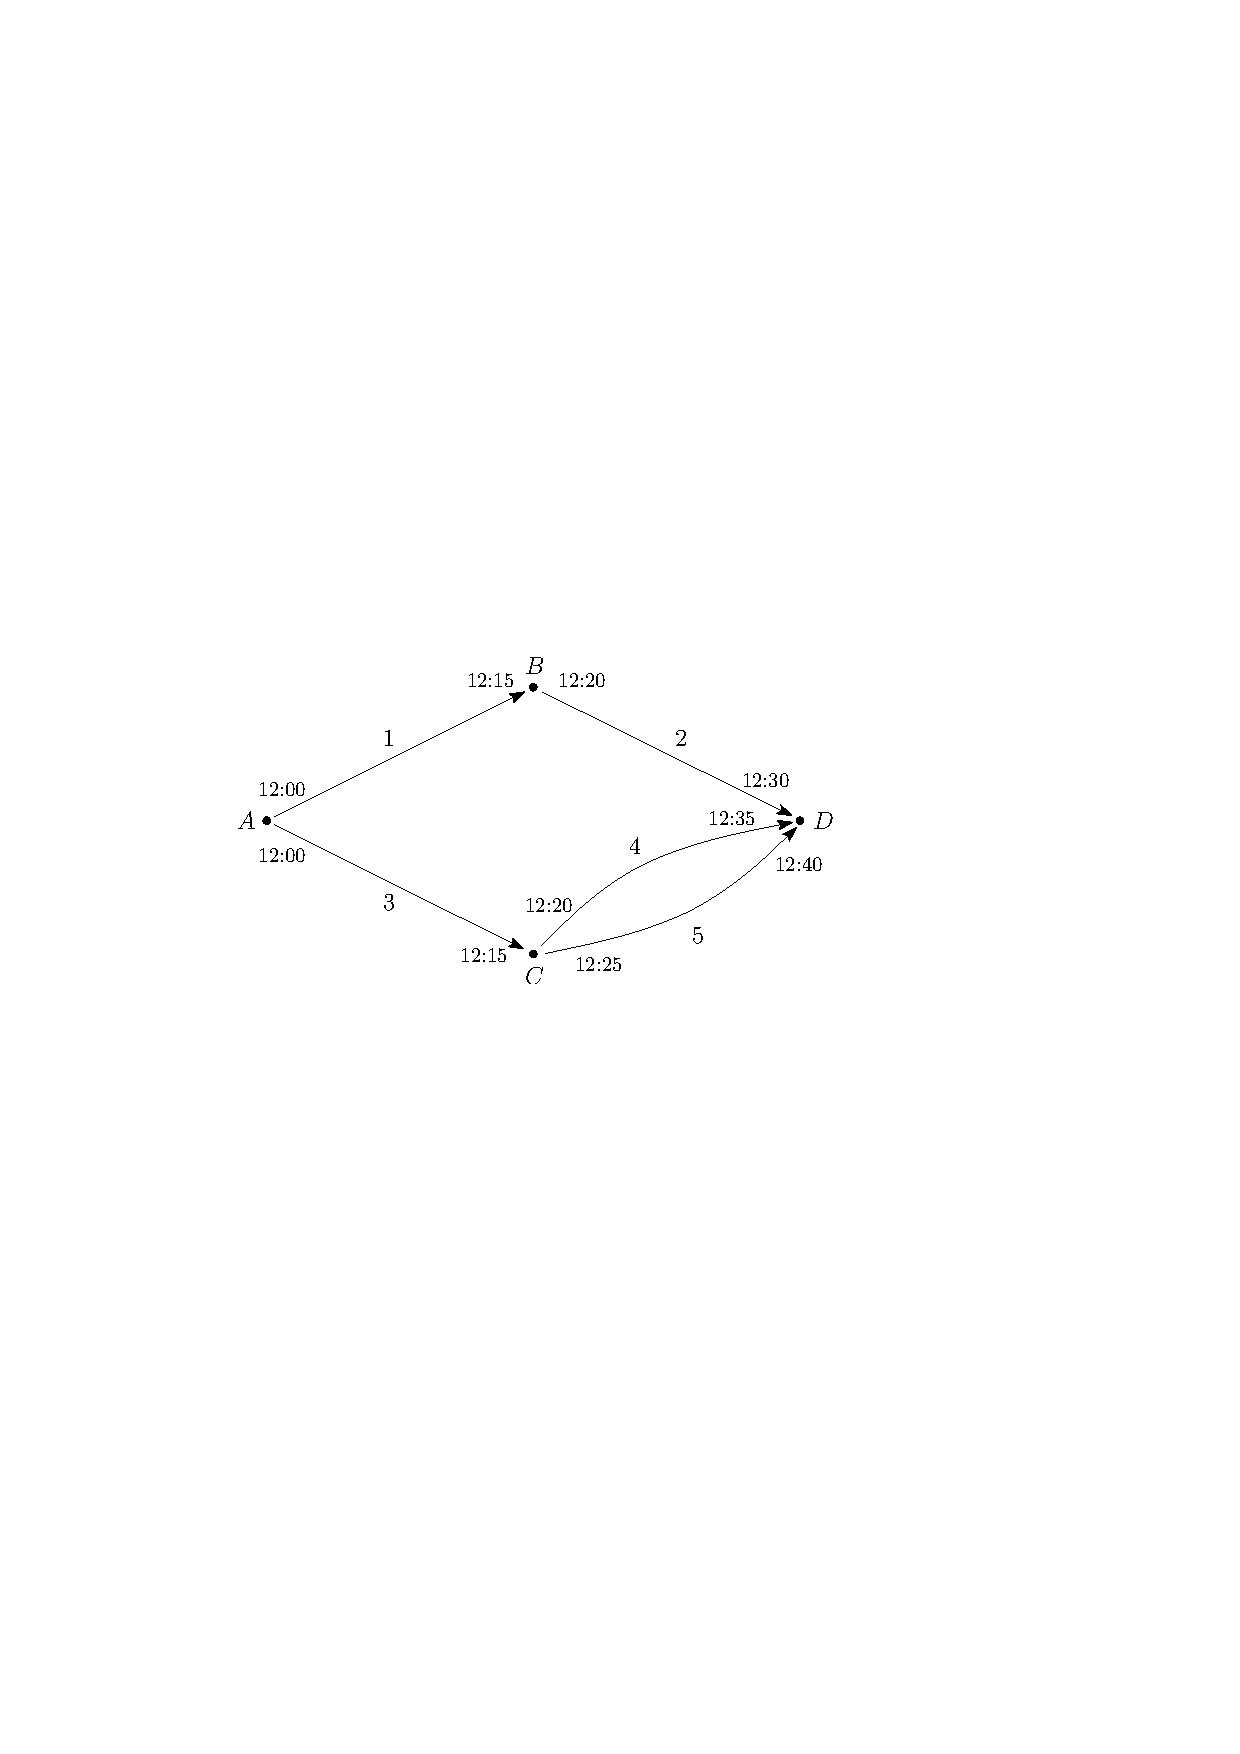
\includegraphics[width=0.9\columnwidth]{stokvsdet01}
\end{center}
\caption{The difference between dynamic and a priori journey planning for a commuter 
traveling from $A$ to $D$. The four points represent public transport stops ($A,B,C,D$) and 
the arrows between them represent public transport services ($1,\ldots,5$).
Initially, there are three possible journeys from $A$ to $D$: $(1,2),(3,4)$ and $(3,5)$.
If the commuter initially chooses service $1$, the success of the journey is 
dependent of the success of the transfer from $1$ to $2$ at stop $B$. If the commuter chooses
service $3$ first, the destination is reached if one of the transfers $3 \to 4$ or $3 \to 5$
is successful at stop $C$.
}
\label{stokvsdet01}
\end{figure}

A simplified example clarifying the main difference between dynamic and a priori journey planning is 
shown in Figure \ref{stokvsdet01}. 

Generally, a commuter wishes to travel from an origin node $v_o$ 
to a destination node $v_d$ within a time horizon $[0,T]$ using different transport services.
Each transport service is represented as a sequence of \emph{legs}. Each leg is associated
with a \emph{start node} and \emph{end node}, as well as a random \emph{start time} and \emph{end time}.
Adjacent nodes in the network are connected with similarly defined walking legs. %, as in \cite{zografos}.

A path from the origin to the
destination is represented as a sequence of legs, in which the start node of
each leg is equal to the end node of the previous leg.
We assume that during the execution of a leg, 
the commuter receives information on which
services have already visited the end node %stop $v_i'$ 
and which are yet to arrive.
In other words, the customer ``sees'' the available successor legs of the current leg
and may choose to (i) stay in the vehicle, %if leg $i$ is not the last leg of the service, 
(ii) transfer to another vehicle or (iii) get off the vehicle and start
walking towards a nearby stop (or the destination).
The goal the above context is to determine an optimal policy specifying the actions
that are executed in different situations in order to 
optimize reliability, ride time, waiting time, walking time, the number of transfers
of a combination of these objectives.

Dynamic path finding problems (see \cite{hall,bander2002,fu1998,miller-hooks2000,davies,kim2005a,kim2005b,azaron,ferris,thomas,waller}) are often modeled
as \emph{Markov decision processes} \cite{psaraftis93,polychronopoulos}, in which the 
\emph{actions} of a decision maker at a given \emph{state} are independent of all previous actions and states.
\ref{jdjuejor} presents a conditional Markov model, in which the path history is included in each state by
defining states as sequences of legs in the transport network.
That is, the current state is determined by the path taken so far.
This model is approximated in \ref{jtoits}, where the current state is defined as the current leg.

The demand-responsive transport service currently being planned to operate in Helsinki
is designed to operate on a demand-responsive basis, that is, 
vehicle routes are modified according to the demand situation. The main difference to existing services is 
that no pre-order times for trips are required and the trips can be booked
``on the fly'' by means of an interactive user interface. 
This type of new service calls for a journey planner that is
capable of communicating with flexible services as well as traditional
public transport, thus combining the benefits of both transport modes.

In addition to public transport, a journey planning problem with a similar objective 
arises in freight transportation by for-hire carriers. 


\section{Stochastic model of a scheduled network [\ref{jdjuejor}]}
Let $\mathcal{V}$ denote a set of \emph{nodes} representing public transport stops
in a specific area and let $\mathcal{K} \subset \mathbb{N}$ denote a set of public 
transport \emph{services} operating in this area, indexed by natural numbers. 

Each service $k \in \mathcal{K}$ follows a \emph{route}, represented as a sequence of nodes $(v_1^k,\ldots,v_m^k)$ in $\mathcal{V}$. 
Each service departs at node $v_1^k$ at a specific time and proceeds to nodes $v_2^k, \ldots,v_m^k$ in the order determined by the route.
Due to uncertainty in departure and travel times, we define the arrival times of services at nodes
as real-valued random variables. Letting $\tau_j^k$ denote the \emph{random arrival time} of 
service $k$ at node $v_j^k$, 
a service $k$ can be represented as a sequence of deterministic nodes and random arrival 
times $((v_1^k, \tau_1^k), \ldots, (v_m^k, \tau_m^k))$, see Figure \ref{stokvsdet02}.
Any two arrival times $\tau_j^k$ and $\tau_l^h$ of 
distinct services $k$ and $h$ are assumed to be independent,
whereas the arrival times $\tau_j^k$ and $\tau_l^k$ of a single 
service $k$ at stops $v_j^k$ and $v_l^k$ are not necessarily independent (see Section \ref{durationmodels}).

\begin{figure}[ht]
\begin{center}
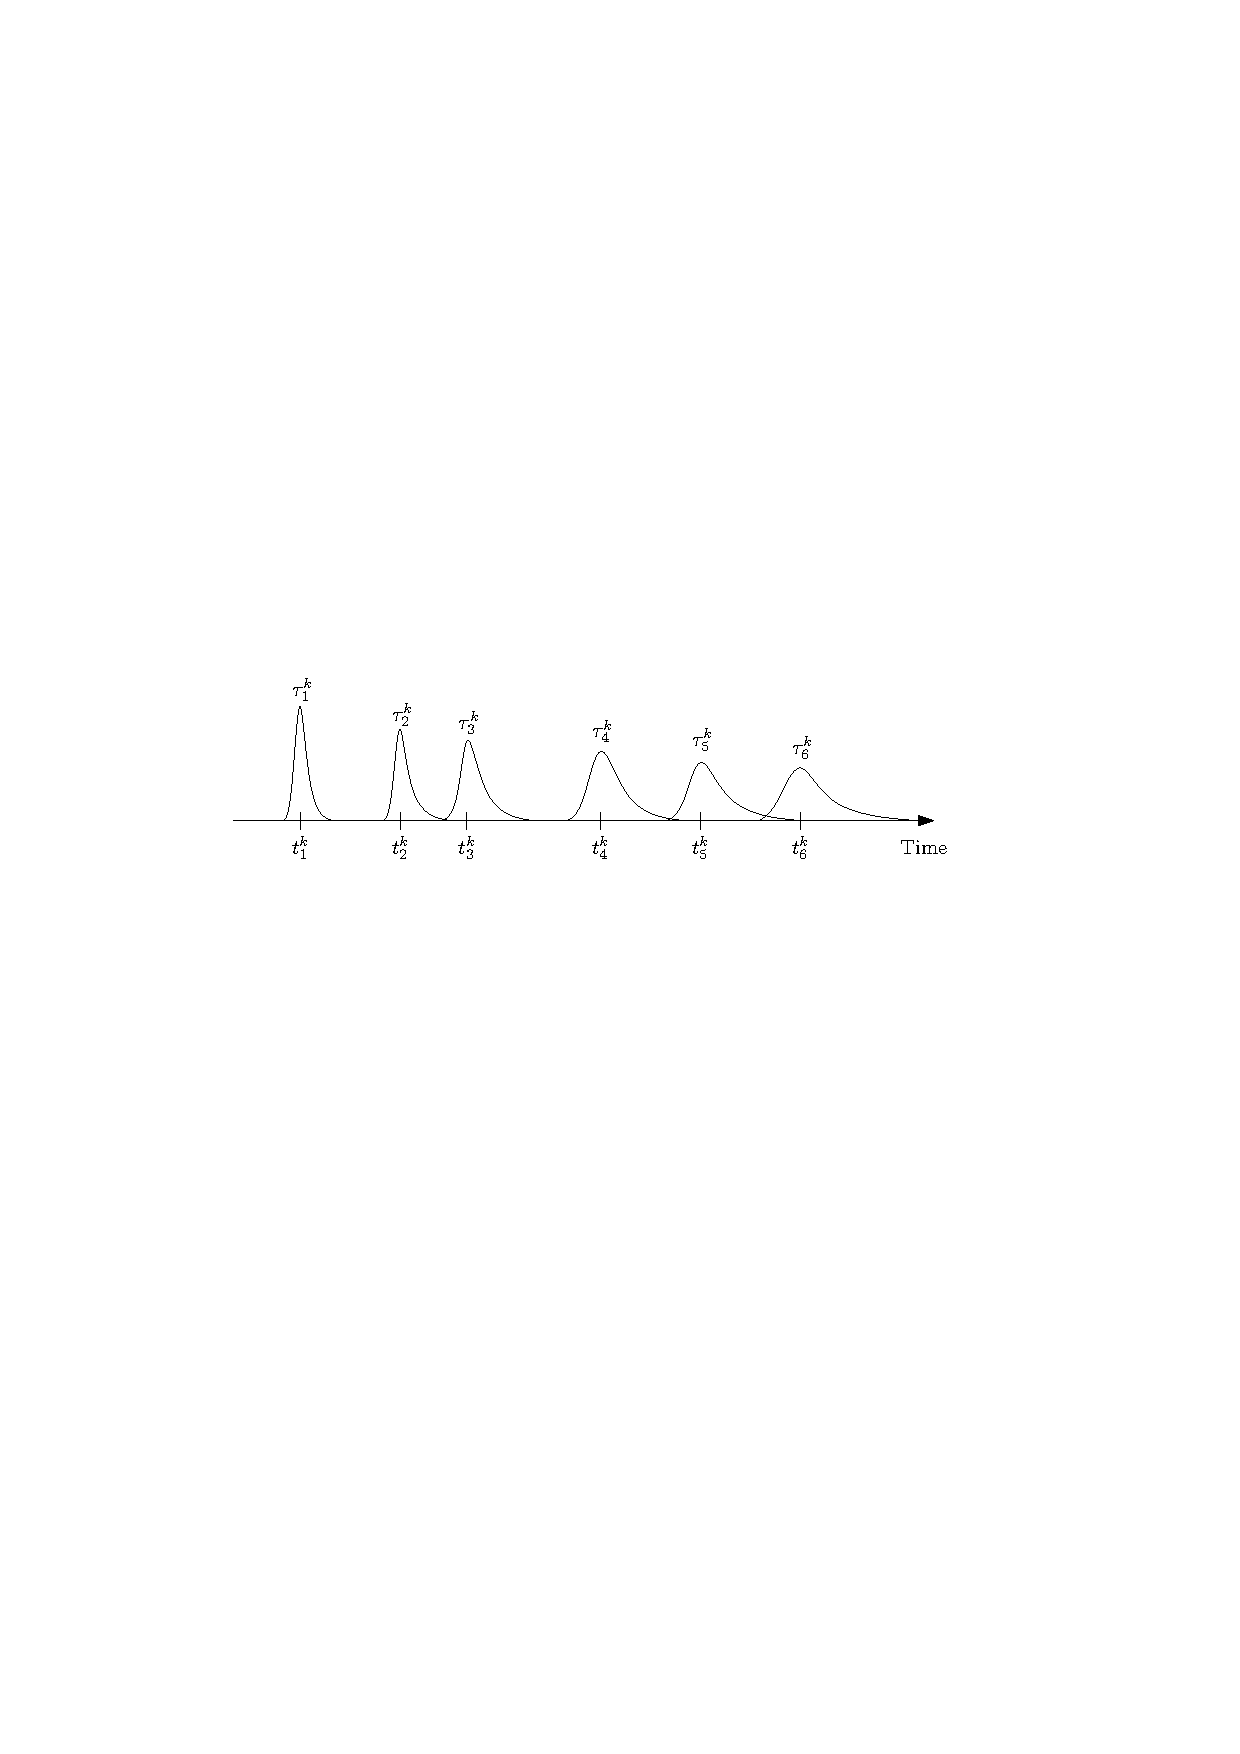
\includegraphics[width=0.9\textwidth]{stokvsdet02}
\end{center}
\caption{The schedule of a transport service. The real numbers $t_j^k$ represent the scheduled arrival
times of a transport service at six subsequent stops. The curves  
represent the distributions of random variables $\tau_j^k$ that are used to model the actual arrival 
times of the service at stops $v_j^k$, $j \in \{1,\ldots,6\}$.}
\label{stokvsdet02}
\end{figure}

\subsection{Service legs}
Each service $k \in \mathcal{K}$ can be decomposed as a set of scheduled \emph{legs} between subsequent stops.
That is, each leg has a start node, end node, start time and end time.
By this decomposition, we can represent any path in the transport network as a sequence 
of legs indexed by natural numbers. For example, consider a transport network consisting of ten legs
numbered from $1$ to $10$. Then, the sequences $(5,2,7)$ and $(5,8,3,7)$ define two paths in the network 
involving two and three \emph{transfers}, respectively. Each transfer between two legs has a specific probability of success.
Transfers between subsequent legs of the same service are assumed to be successful with 
probability $1$.

Formally, letting $\mathcal{L} \subset \mathbb{N}$ denote the set of indices of legs, 
a leg corresponding to index $i \in \mathcal{L}$ is defined by a pair of 
node-arrival time pairs and a service number $((v_i, \tau_i), (v_i', \tau_i'), k_i)$,
where $v_i$ is the \emph{start node}, $v_i'$ is the \emph{end node}, $\tau_i$ is the \emph{start time}, $\tau_i'$ 
is the \emph{end time} and the \emph{service number} $k_i$ is the index of the service that executes leg $i$.

By using this definition, a service  $((v_1^k, \tau_1^k), \ldots, (v_m^k, \tau_m^k))$ is
represented by a set of legs ${\{i_1^k,\ldots,i_{m-1}^k\} \subset \mathcal{L}}$, where leg $i_h^k$
is determined by 
\begin{align}
\label{legdefinition}
\left( (v_{i_h^k}, \tau_{i_h^k}), (v_{i_h^k}', \tau_{i_h^k}'),k_{i_h^k} \right) 
= \left((v_{h}^k, \tau_{h}^k),(v_{h+1}^k, \tau_{h+1}^k),k \right)
\end{align}
for $h \in \{1,\ldots , m-1\}$. 
Note that the end time $\tau_{i_h^k}'$ of leg $i_h^k$ refers to 
the same specific random variable as the start time $\tau_{i_{h+1}^k}$ of leg $i_{h+1}^k$, that is, 
$\tau_{i_h^k}' = \tau_{i_{h+1}^k} = \tau_{h+1}^k$. 
To keep track which legs are subsequent
legs of the same service, we define for each leg $i_h^k$ the \emph{set
of immediate successors} $I_{i_h^k} = \{ i_{h+1}^k\}$ for $h \in \{1,\ldots , m-1\}$.

\subsection{Walking legs}
After each leg traversed, a commuter may choose to continue the journey by foot. 
Similarly as the service legs defined above, each \emph{walking leg} $i \in \mathcal{L}$ 
is determined by a start node $v_i$, end node $v_i'$, start time $\tau_i$, end time $\tau_i'$ 
and service number $k_i$. For all walking legs, we choose $k_i < 0$ in order to have a distinction 
between walking legs and service legs.

Walking legs are added by associating with each service leg $((v_i, \tau_i), (v_i', \tau_i'),k_i)$ a set 
$L_i \subset \mathcal{L}$ of walking legs beginning at $v_i'$ and ending at a stop within a specific 
\emph{maximum walking distance} $d_w^{\max }$ from $v_i'$, see Figure \ref{walking01}a. Such walking legs $j \in L_i$
are of the form
$
\left((v_j, \tau_j), (v_j', \tau_j'),k_j\right)=\left( (v_i', \tau_i'),(v_j',\tau_j'),-k_i \right),
$
where the walking distance $d_w$ satisfies $d_w(v_i',v_j') \leq d_w^{\max }$. % and
Note that the end time $\tau_i'$ of service leg $i$ and the start time $\tau_j$ of a walking leg $j \in L_i$
refer to the same specific random variable. 
For each service leg $i$, the walking legs are added to the set of immediate
successors $I_{i}$ of $i$, that is, $I_{i} \leftarrow I_{i} \cup L_i$.

\begin{figure}[ht]
\begin{center}
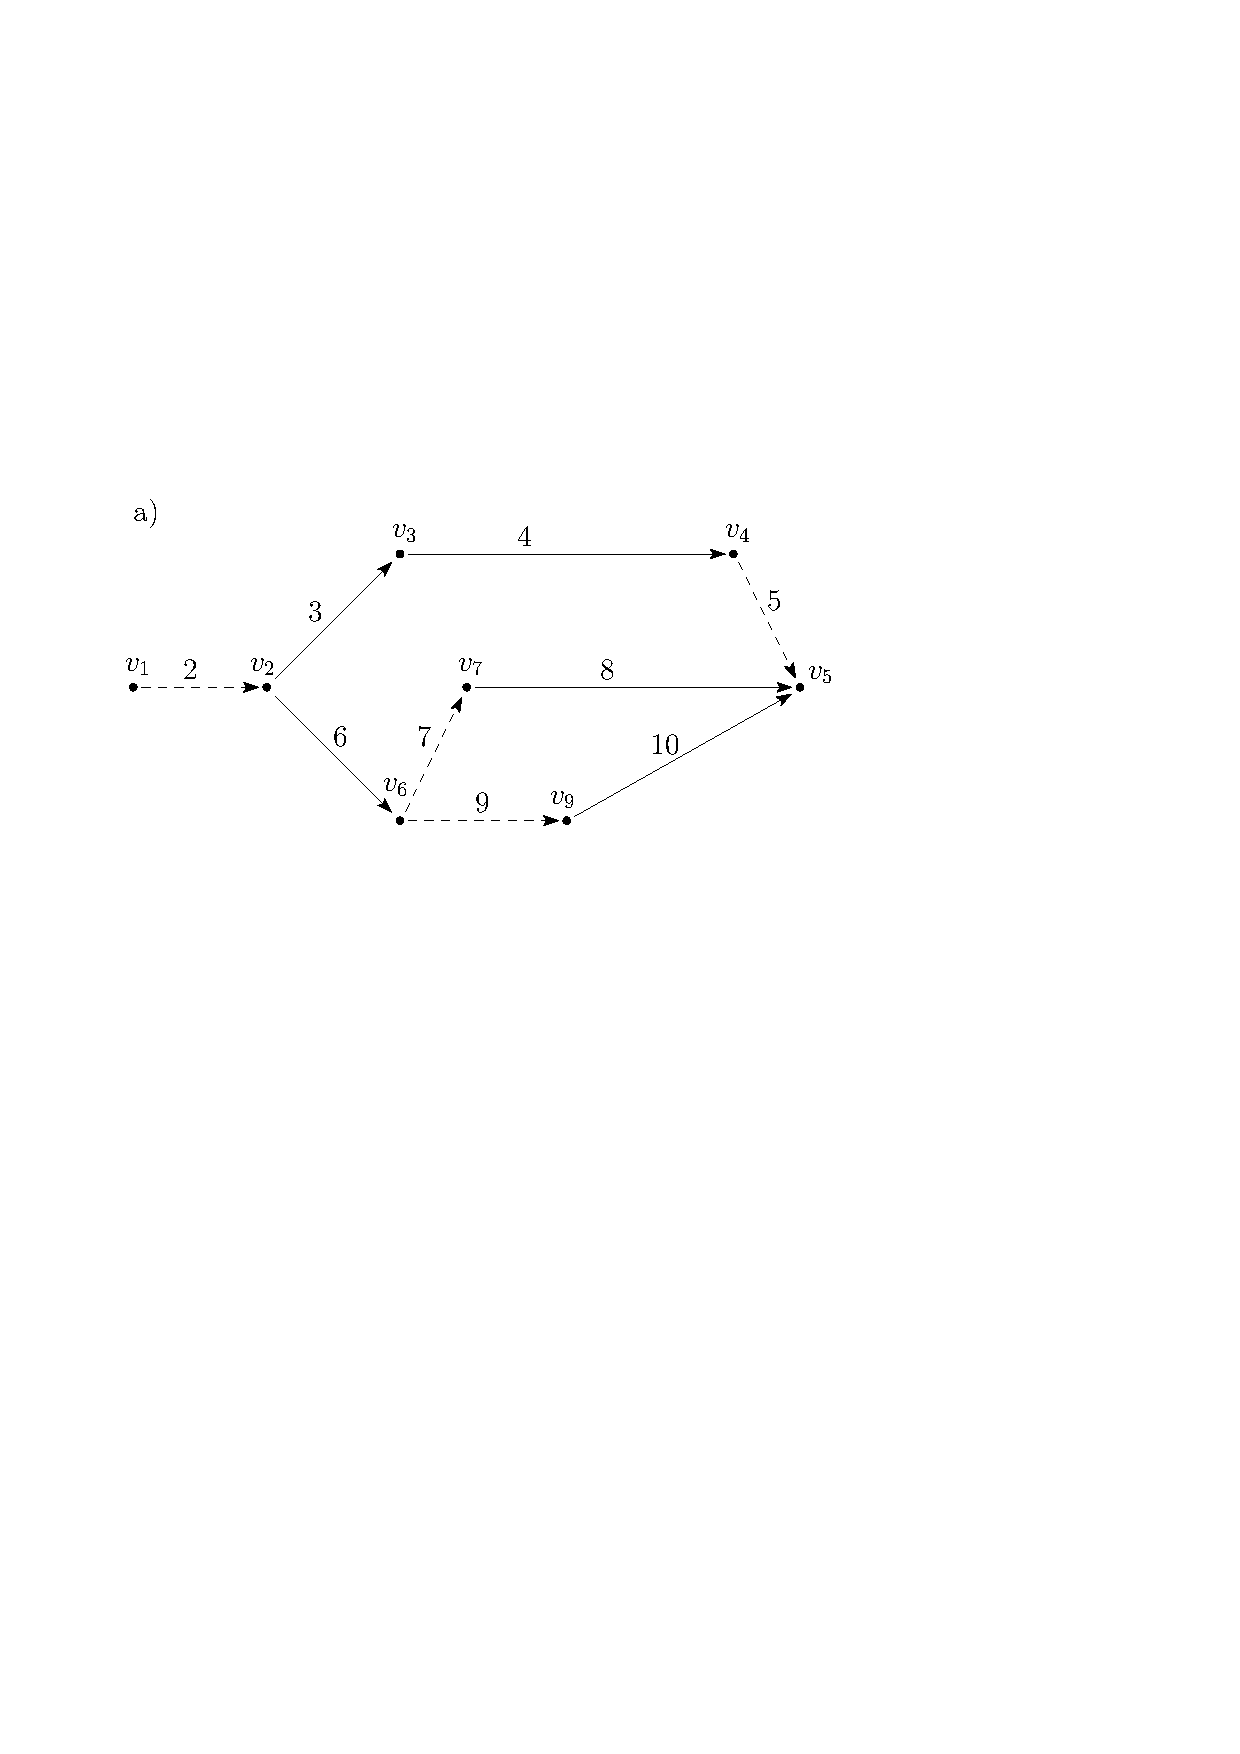
\includegraphics[width=0.45\textwidth]{walking01}
\ \ \ \ \ \ \ 
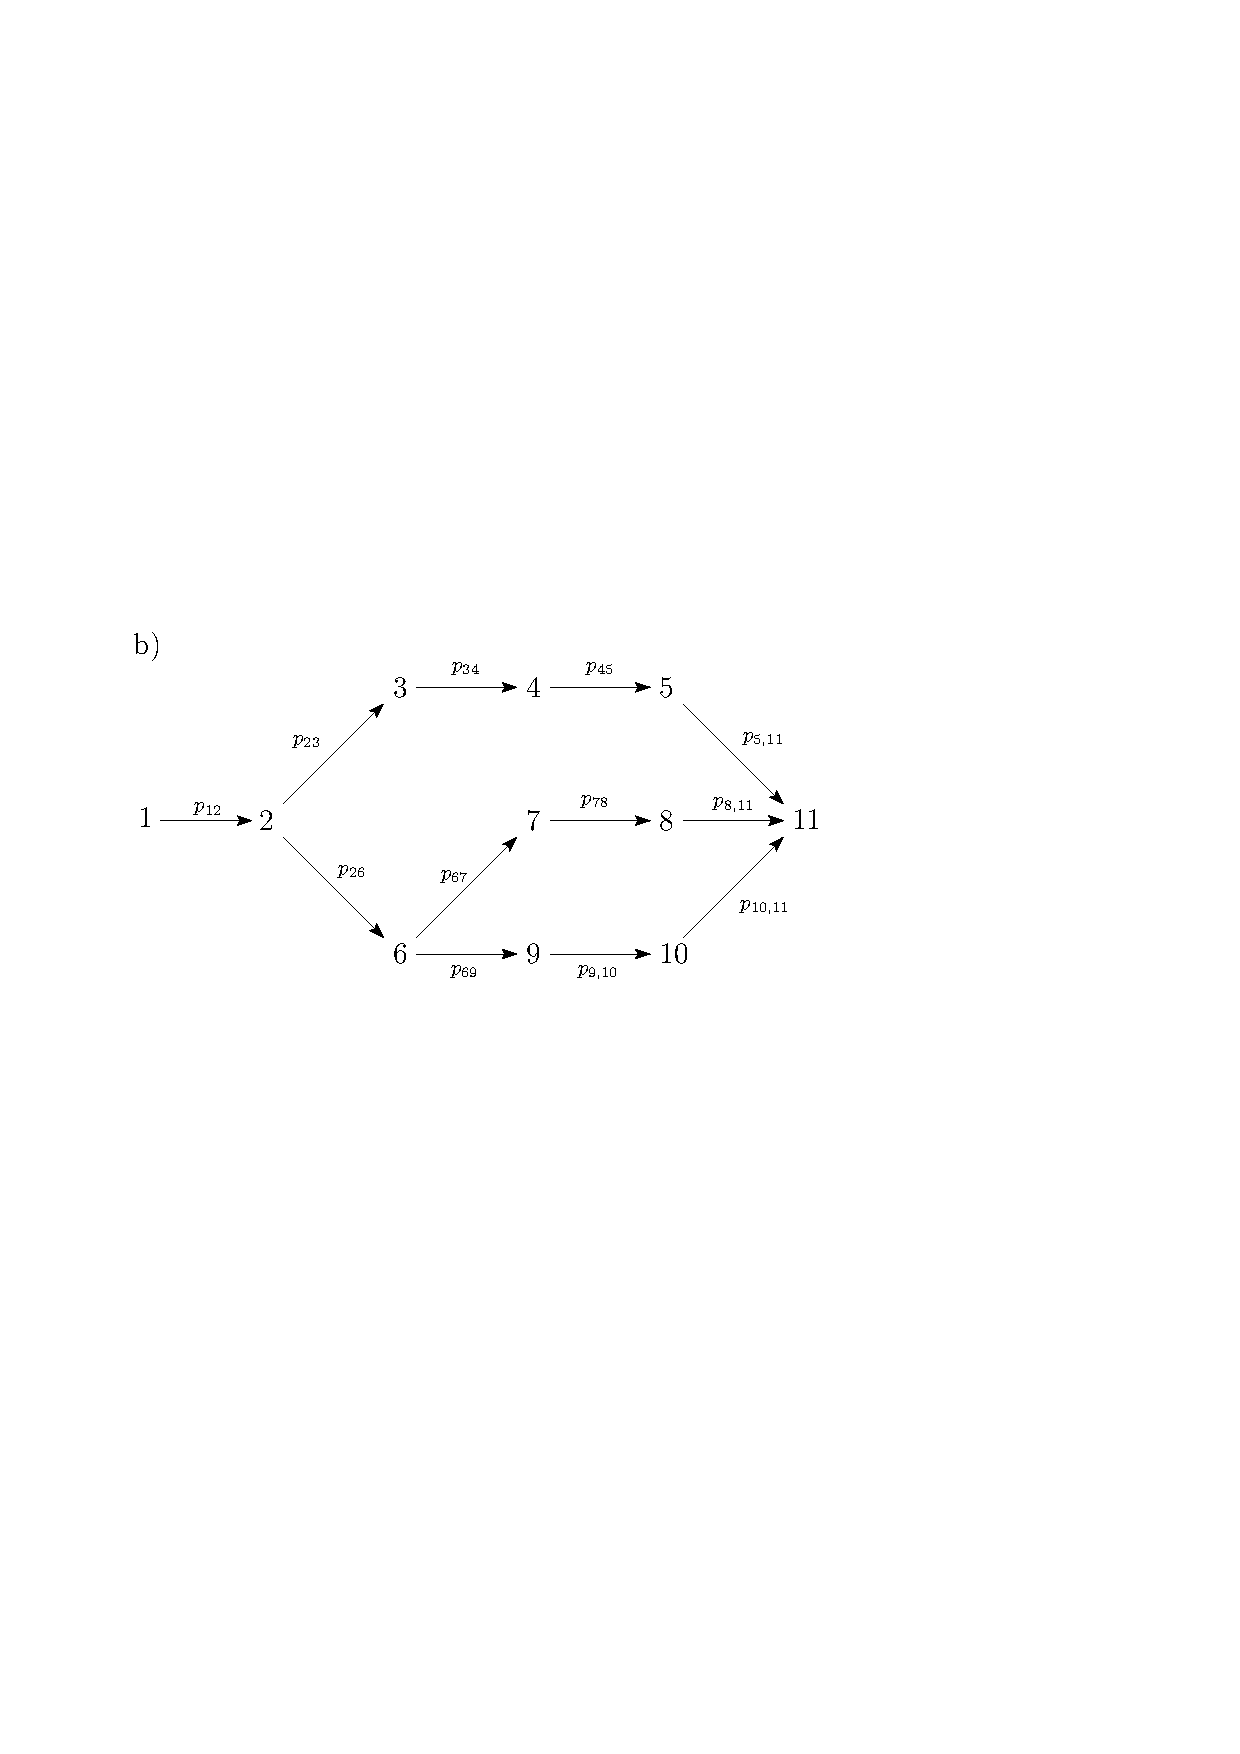
\includegraphics[width=0.45\textwidth]{walking01c}
\end{center}
\caption{a) A sample transport network with eight stops and five 
transport services consisting of a single leg (solid arrows $3,4,6,8,10$).
Adjacent stops are connected with walking legs (dashed arrows $2,5,7,9$).
b) A directed graph representing the relations of legs in Figure \ref{walking01}a. 
The origin and destination are represented by legs $1$ and $11$. 
%Note that legs $1$ and $5$ have two successors whereas the other legs have a single successor.
The prior transfer probability from leg $i$ to leg $j$  is denoted by $p_{ij}$.
Note that $p_{12}=p_{45}=p_{67}=p_{69}=1$, since $2,5,7$ and $9$ are walking legs.
}
\label{walking01}
\end{figure}

Sequential walking legs are added to the network iteratively:
First, walking legs (indexed with service number $-k_i$) are added to the end of each each service leg $i$ (step 1).
Then, walking legs (indexed with service number $k_j$) are added to the end of each walking leg $j$ (step 2).
Step 2 is repeated until the desired amount of walking legs is obtained.
The number of walking legs included in the model is thus controlled by two parameters:
The maximum walking distance $d_w^{\max }$ and the maximum number of sequential walking legs.


\subsection{Transfer probability}
A transfer from leg $i$ to leg $j$ is possible only if leg $i$ ends at the node from which leg $j$ begins, that is, $v_{i}' = v_{j}$ (see Figure \ref{walking01}b).
Letting $\mathcal{L}$ denote the set of legs and $S_i = \{j \in \mathcal{L} \ | \ v_{i}' = v_{j} \}$ denote the 
\emph{successor set} of leg $i$,
%In this case, 
the \emph{prior transfer probability} from leg $i$ to leg $j$ is defined by
\begin{align}
\label{transferprob}
p_{ij}=
\left\{
\begin{array}{ll}
P(\tau_{i}' \leq \tau_{j}), & \mbox{if $j \in S_{i}$}, \\
0, & \mbox{otherwise.}
\end{array}
\right.
\end{align}

Note that if $j$ is a walking leg beginning at the end of leg $i$
or if $i$ and $j$ are successive legs of the same service,
by definition we have $p_{ij}= 1$, since $\tau_{i}'$ and $\tau_{j}$ refer to the same random variable. 
The legs and prior transfer probabilities
form a directed graph (Figure \ref{walking01}b).

More generally, since the start and end time of a leg are not necessarily independent, 
the transfer probability from $i$ to $j$ depends on the \emph{path} taken to get to $i$.
A path can be represented as an acyclic sequence of legs $(i_1,\ldots,i_m)$ satisfying
$i_{h+1} \in S_{i_h}$ for all $h \in \{1,\ldots,m-1\}$, see Figure \ref{journey01}. 
The path is \emph{successful}, if $\tau_{i_h}' \leq \tau_{i_{h+1}}$ for all $h \in \{1,\ldots,m-1\}$.

\begin{figure}[ht]
\begin{center}
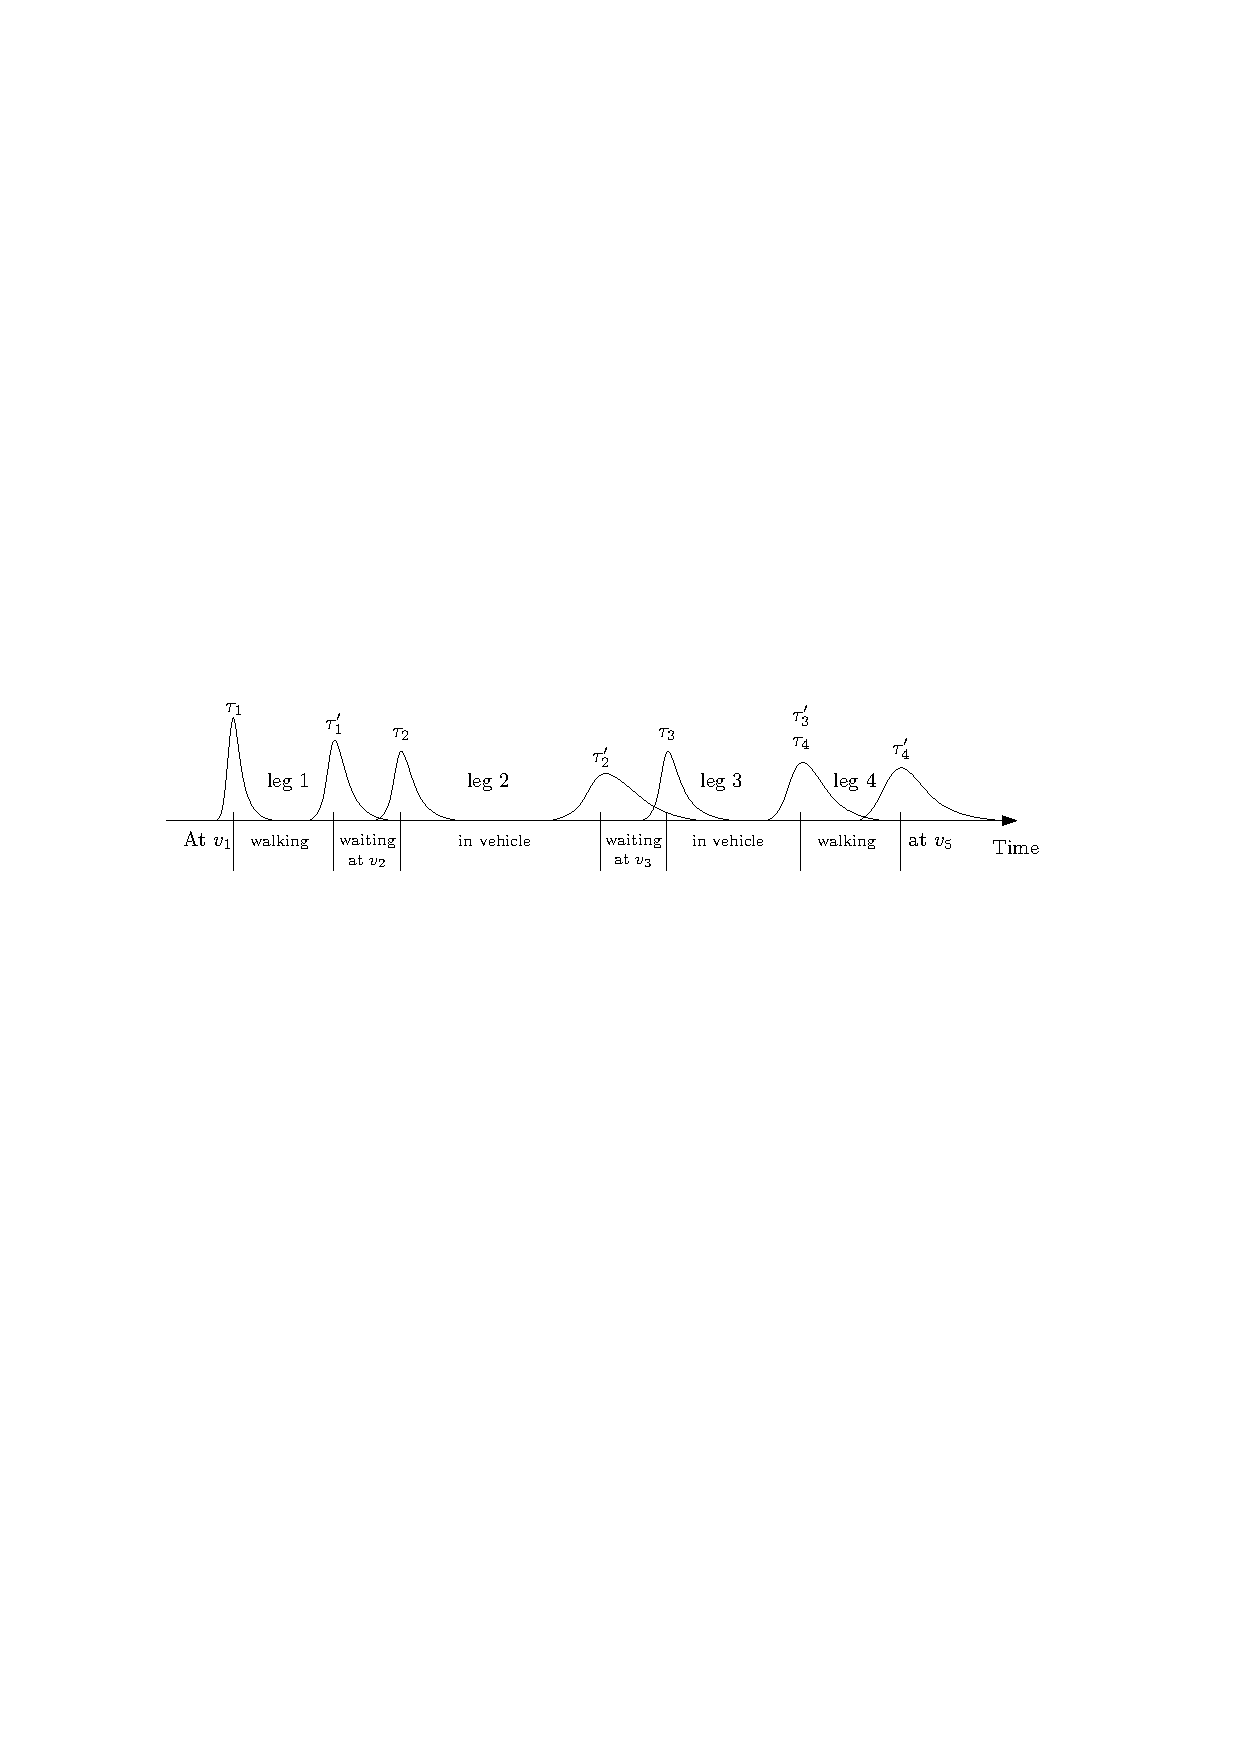
\includegraphics[width=0.9\textwidth]{journey02}
\end{center}
\caption{Deterministic and stochastic representations of a path. The ticks on the time axis represent the 
schedule of a deterministic itinerary from $v_1$ to $v_5$. The curves represent the distributions 
of random variables $\tau_i, \tau_i'$ that are used to model the start and end times of four legs that 
define the corresponding stochastic path. 
(1) A commuter starts walking at $\tau_1$ from the origin $v_1$, and arrives at stop $v_2$ at $\tau_1'$. 
(2) A transport service departs at $v_2$ at $\tau_2$ and travels to stop $v_3$,
arriving at $\tau_2'$. (3) A transport service departs at $v_3$ at $\tau_3$ and arrives at stop $v_4$ at $\tau_3'$. 
(4) Immediately at $\tau_4=\tau_3'$, 
the commuter continues by foot to the destination $v_5$, arriving at $\tau_4'$. Note that the path is successful
with probability 
$P(\tau_1' \leq \tau_2 \cap \tau_2' \leq \tau_3) 
= P(\tau_1' \leq \tau_2) \cdot P (\tau_2' \leq \tau_3 \ | \ \tau_1' \leq \tau_2)$.
}
\label{journey01}
\end{figure}


\section{Problem formulation and solution}
The dynamic journeying problem is defined as follows.
Let $[0,T] \subset \mathbb{R}$ be the time horizon of the problem,
let $v_1$ denote the origin node and $v_d$ denote the destination node. 
The \emph{origin leg} is defined by $((v_1,\tau_1),(v_1,\tau_1),0)$, where $P(\tau_1=0)=1$, 
and the \emph{destination leg} 
is defined by $((v_{d},\tau_{d}),(v_{d},\tau_{d}),0)$, where $P(\tau_d=T)=1$.
Although it is possible to reach the destination node before $T$, the start time of the 
destination leg equals $T$ with probability $1$. By this definition, we can represent the entire journey 
as legs, including the origin and the destination. If a journey ends at a successful transfer 
to the destination leg, we know that the commuter has reached the destination node before $T$ or at $T$.

With no loss of generality, all legs for
which the start or end time is outside the time horizon $[0,T]$ with probability $1$ and 
all legs for which the start node is the destination node (except the destination leg)
are excluded from the problem.
The cropped set of legs is defined by 
\begin{align*}
\mathcal{L}_{[0,T]}= \left\{i \in \mathcal{L} \ | \ P( 0 \leq \tau_i \leq T) > 0 \mbox{ and } P( 0 \leq \tau_i' \leq T) > 0\right\}
\setminus \{i \in \mathcal{L} \setminus \{d\} \mid v_i = v_d\}.  
\end{align*}
For clarity, we define $n:=|\mathcal{L}_{[0,T]}|$ and the legs in $\mathcal{L}_{[0,T]}$ 
are numbered from $1$ to $n$, where the origin leg is indexed by $1$ and the destination leg is indexed by $n$.

\subsection{Markov decision process}
The problem is modeled as a finite-state Markov decision process $(S,A,P_{\cdot}(\cdot,\cdot),R_{\cdot}(\cdot,\cdot))$, 
where the parameters are defined as follows.

\subsubsection{States}
\label{statesdef}
The set of \emph{states} $S$ consists of paths $(1,i_1,\ldots,i_m)$ of legs, where $i_h \in \{1,\ldots,n\}$ for $h \in \{0,\ldots,m\}$,
beginning from the origin leg $1$. The state $(1)$ is referred to as the \emph{origin state}.
Each state $s=(i_0,i_1,\ldots,i_m) \in S$, where $i_0=1$, is associated with a set of successor states
$S_{s} = \{(i_0,i_1,\ldots,i_m,j)\in S \mid j \in S_{i_m} \}$, where $S_{i_m}$ is the successor set of leg $i_m$.
Similarly, the set of immediate successors of state $s$ is defined by
$I_{s} = \{(i_0,i_1,\ldots,i_m,j)\in S \mid j \in I_{i_m} \}$, where $I_{i_m}$ is the immediate successor set of leg $i_m$.
Formally, the set of states is defined by
\begin{align}
\label{statejoukko}
 S=\left\{(i_0,\ldots,i_m) \mid i_0=1 \mbox{ and } i_{h+1} \in S_{i_h} \mbox{ for } h \in \{0,\ldots,m-1\} \right\}.
\end{align}
The above definition of a state includes travel history in the form of a path, see Figure \ref{treemodel01}. 
The history of performed actions is not taken into account in the model.

\begin{figure}[ht]
\begin{center}
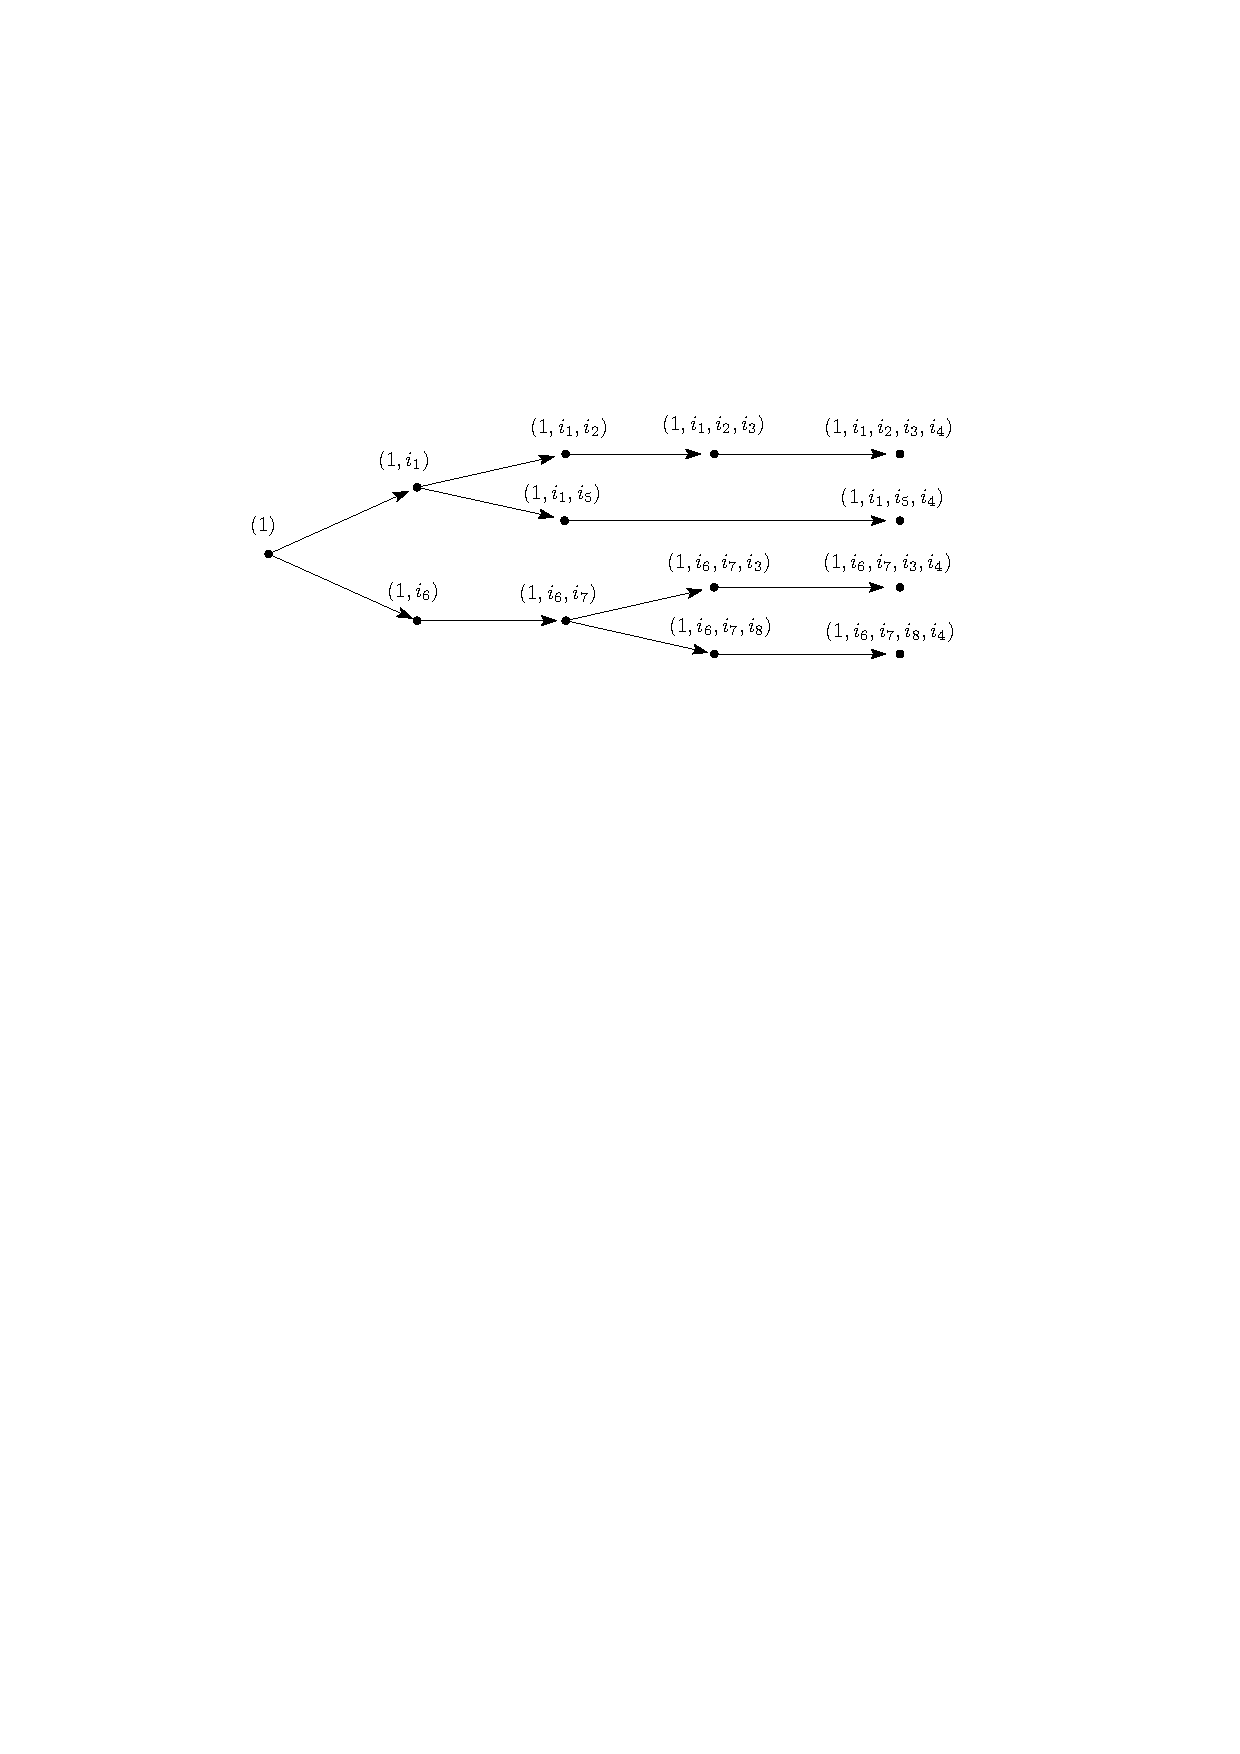
\includegraphics[width=0.9\textwidth]{treemodel01}
\end{center}
\caption{
States of the markov decision process. A state is defined as a path consisting of legs, beginning from the origin leg $1$.
The states $s$ in the figure are connected to successor states $s' \in S_s$ by arrows.
Since the travel history is included in the definition of a state, the state space has a tree structure.
In this example, the destination leg is denoted by $i_4$  and the set of destination states equals
$\mathcal{D} = \{(1,i_1,i_2,i_3,i_4),(1,i_1,i_5,i_4),(1,i_6,i_7,i_3,i_4),(1,i_6,i_7,i_8,i_4)\}$.
}
\label{treemodel01}
\end{figure}

The set of \emph{destination states}, that is, the set of states $(1,\ldots,i_m) \in S$ for which the last leg $i_m$ 
is the destination leg, is defined by $\mathcal{D} = \left\{(1,\ldots,i_m) \in S \mid i_m=n  \right\}$.
Since legs beginning from the destination node are not included in the problem, we have $S_s = I_s = \emptyset$ for all $s \in \mathcal{D}$.

The start and end times of state $s$ are denoted by the random variables $\tau_s$ and $\tau_s'$, respectively.
The distributions of $\tau_s$ and $\tau_s'$, where $s=(i_0,i_1,\ldots,i_m)$ and $i_0=1$, are defined by
\begin{align}
\label{ehdollinen1}
f_{\tau_s }(x) &= f_{\tau_{i_m}} (x  \mid \cap_{h=0}^{m-1} \tau_{i_h}' \leq \tau_{i_{h+1}} ), \\
\label{ehdollinen2}
f_{\tau_s'}(x) &= f_{\tau_{i_m}'}(x \mid  \cap_{h=0}^{m-1} \tau_{i_h}' \leq \tau_{i_{h+1}} ),
\end{align}
for $x \in \mathbb{R}$.
The service number of state $s=(i_0,i_1,\ldots,i_m)$ is defined by $k_s = k_{i_m}$.

\subsubsection{Actions}
\label{actionsdef}
The set of \emph{actions} $A$ consists of sets $A_s$ of actions available at states $s \in S$.
An action $a \in A_s$ is defined as a \emph{preference order} of the successor states $s' \in S_s$, 
that is, a bijection $a:S_s \to \{1,\ldots,|S_s|\}$, where $a(s')$ denotes the ranking of the successor state $s' \in S_s$
in the preference order. The successor states of $s$ ranked by the preference order $a$ are denoted by $s^{a,a(s')}$.
Given the the sorted successor states $s^{a,1}, \ldots, s^{a,|S_s|} \in S_{s}$ of $s$, 
the commuter transfers to state $s^{a,k}$ if 
(i) the transfer to $s^{a,g}$ is unsuccessful for $1 \leq g < k$ and 
(ii) the transfer to $s^{a,k}$ is successful.

\subsubsection{Transition probabilities}
\label{transitiondef}
$P_a(s,s') = P(s_{t+1}=s' \mid s_t = s, a_t=a)$ is the probability that action $a$ in state $s$ 
at step $t$ will lead to state $s' \in S_s$ at step $t + 1$. 
Given the preference order $s^{a,1}, \ldots, s^{a,|S_s|} \in S_{s}$ defined by action $a \in A_s$, 
we have 
\begin{align}
\label{ekakaava}
P_a(s,s^{a,k}) 
= 
P\left(\tau_{s}' \leq \tau_{s^{a,k}} \cap \bigcap_{g=1}^{k-1} \tau_{s}' > \tau_{s^{a,g}} \right).
\end{align}
If the service numbers of all pairs of distinct successor states $s',s'' \in S_s$ of state $s$ satisfy $k_{s'} \neq k_{s''}$,
we have 
\begin{align*}
P_a(s,s^{a,k}) = \int_{-\infty}^{\infty} f_{\tau_{s}'}(x) P\left(x \leq \tau_{s^{a,k}} \right) 
\prod_{g=1}^{k-1} P\left(x > \tau_{s^{a,g}} \right) \ dx,
\end{align*}
since the start times of legs with different service numbers 
are independent.
Note that since the end time $\tau_s'$ of state $s$ and the start time of an immediate successor state $s' \in I_s$ refer to the same
random variable, that is, $\tau_s' = \tau_{s'}$ for all $s' \in I_s$, the transfer probability \eqref{ekakaava}
satisfies
\begin{align}
\label{ekakaava2}
P_a(s,s^{a,k}) = 
\left\{
\begin{array}{ll}
0, &  \mbox{if $\{s^{a,1},\ldots,s^{a,k-1}\} \cap I_s \neq \emptyset$ },\\ 
P\left(\bigcap_{g=1}^{k-1} \tau_{s}' > \tau_{s^{a,g}} \right), &  \mbox{if $\{s^{a,1},\ldots,s^{a,k-1}\} \cap I_s = \emptyset$ and $s^{a,k} \in I_{s}$ },\\ 
P\left(\tau_{s}' \leq \tau_{s^{a,k}} \cap \bigcap_{g=1}^{k-1} \tau_{s}' > \tau_{s^{a,g}} \right), & \mbox{otherwise.}
\end{array}
\right.
\end{align}
For example, let $s^{a,1},s^{a,2},s^{a,3}$ denote three successor states of state $s$, sorted in the preference
order defined by action $a$. If $s^{a,2}$ is an immediate successor of $s$, that is, $s^{a,2} \in I_s$, and $s^{a,1} \notin I_s$, 
we have $P_a(s,s^{a,1}) = P\left(\tau_{s}' \leq \tau_{s^{a,1}} \right)$, $P_a(s,s^{a,2}) = P\left( \tau_{s}' > \tau_{s^{a,1}} \right)$
and $P_a(s,s^{a,3}) = 0$.

\subsubsection{Rewards}
\label{rewardsdef}
$R_a(s,s')$ is the expected immediate reward received after transition from state $s \in S$ to state $s' \in S$ 
with transition probability $P_a(s,s')$. 
Since the objective is to arrive at a destination state $s \in \mathcal{D}$, we define $R_a(s,s')$ by
\begin{align}
\label{rewards}
 R_a(s,s')= 
\left\{
\begin{array}{ll}
1, &  \mbox{if $s' \in \mathcal{D}$ },\\ 
0, & \mbox{otherwise.}
\end{array}
\right.
\end{align}
Note that $R_a(s,s')$ is independent of the action $a$. Thus, for the remainder of this document, we will use
the notation $R(s,s') = R_a(s,s')$.

Travel and overdue costs can be included in the reward function with minimial effort as follows.
Instead of maximizing the probability of reaching the destination leg, the goal is to 
maximize the expected profit gained by arriving at the destination node.

Let $u$ denote the revenue (or utility) received upon arrival at the destination node and $c(s)$ 
denote a real valued positive function representing the cost of state $s$. 
For example, $c((i_0,\ldots,i_m))$ could be defined as the sum of the \emph{leg costs} $c_{i}$,
that is, \\ ${c((i_0,\ldots,i_m))= \sum_{h=0}^{m-1} c_{i_h}}$ or a combination of ride time, waiting time, walking time and the 
number of transfers, as in \ref{jtoits}. 
Let $C_o$ denote the \emph{overdue cost}, 
that is, the cost of arriving at the destination node after $T$. By introducing an
additional \emph{late destination leg} $((v_{d},\tau_{l}),(v_{d},\tau_{l}),0)$, where $P(\tau_l=\infty)=1$,
and the set of \emph{late destination states} $\mathcal{D}'$, for which the last leg is the late destination leg,
the reward function is written in the general form
\begin{align}
\label{rewards2}
 R'(s,s')= 
\left\{
\begin{array}{ll}
u - c(s'), &  \mbox{if $s' \in \mathcal{D}$ },\\ 
u - c(s') - C_o, &  \mbox{if $s' \in \mathcal{D}'$ },\\ 
0, & \mbox{otherwise.}
\end{array}
\right.
\end{align}


\subsection{Optimal policy}
\label{solution}
The solutions to Markov decision processes are characterized as policies, 
that is, functions $\pi$ that specify the action 
$a(s)$ that the commuter chooses when in state $s$. 
The goal is to find a policy $\pi$ that maximizes the expected reward. 
Generally, the calculation of an optimal policy requires two arrays indexed by state: 
value $V$, which contains real values, and policy $\pi$ which contains actions. 
%In our problem, $V(s)$ corresponds to the probability of reaching a destination state $s' \in \mathcal{D}$
%from state $s$ by following a policy that maximizes the expected reward.

Similarly as in \citep{bellman}, the value $V(s)$ is defined by 
\begin{align}
\label{rekursio01}
V(s) := \max_{a \in A_s} \left\{ \sum_{s' \in S_s} P_a(s,s') \left(R(s,s') +V(s')\right)\right\}
\end{align}
for all $s \in S$. Note that $V(s)=0$ for all $s \in \mathcal{D}$, since $S_s = \emptyset$ for all $s \in \mathcal{D}$.

An optimal policy is characterized as follows:
When at state $s$, the available transfer options $X \subset S_s$ to successor states are revealed.
The commuter transfers to a state $s' \in X$ for which $R(s,s') +V(s')$ is maximized.
Formally, an optimal action $a$ at state $s$ is determined by
the following theorem.

\begin{theorem}
\label{optimalpolicy}
Let $s \in S$ be a state. An action $a \in A_s$ is optimal satisfying Equation \eqref{rekursio01}, if 
\begin{align}
\label{jarjestys}
R(s,s^{a,1})+V(s^{a,1}) \geq R(s,s^{a,2})+V(s^{a,2}) \geq \ldots \geq R(s,s^{a,|S_s|})+V(s^{a,|S_s|}),
\end{align}
where the successor states ranked by action $a$ are denoted by $s^{a,a(s')}$ for all $s' \in S_s$.
\end{theorem}
Theorem \ref{optimalpolicy} gives an optimal action
for a state $s$, given that the values $V(s')$ of its successor states are known.
In the following, we present an algorithm for calculating the values for all states.

\subsection{Backward induction algorithm}
The values $V(s)$ of states can be determined
by means of backward induction, as shown in Algorithm \ref{backward01}.
By executing Val($(1)$), the program recursively calculates values and optimal actions for 
all states $s$ that are reachable from the origin state $(1)$.

Initially, we only know the values of destination states, that is, $V(s)=0$ for all $s \in \mathcal{D}$.
Thus, the first states for which the value can be calculated
are the ones that precede a destination state. 
The algorithm then proceeds backwards until the value $V((1))$ of the origin state is calculated.

\begin{algorithm}
\begin{algorithmic}
 \FORALL {$s' \in S_{s}$ (successor set of $s$)}
\STATE $V(s') \leftarrow $ Val($s'$);
\STATE Determine an optimal action $a$ by sorting the states $s' \in S_{s}$ in descending order of $R(s,s') + V(s')$;
\STATE $V(s) \leftarrow \sum_{k=1}^{|S_s|} P_{a}(s,s^{a,k}) \left( R(s,s^{a,k}) +V(s^{a,k}) \right)$ \hfill ($V(s) = 0$ for destination states);
\STATE Return $V(s)$;
\ENDFOR
\end{algorithmic}
\caption{A recursive function Val($s$) for calculating the value $V(s)$ for state $s$.}
\label{backward01}
% {\scriptsize
% \ForAll{$s' \in S_{s}$ (successor set of $s$)}{
% $V(s') \leftarrow $ Prob($s'$)\; 
% }
% Determine an optimal action $a$ by sorting the states $s' \in S_{s}$ in descending order of $R(s,s') + V(s')$\;
% $V(s) \leftarrow \sum_{k=1}^{|S_s|} P_{a}(s,s^{a,k}) \left( R(s,s^{a,k}) +V(s^{a,k}) \right)$ \hfill ($V(s) = 0$ for destination states)\;
% Return $V(s)$\;
% }
\end{algorithm}



\section{Analysis}
\label{analysis}
\ref{jdjuejor} presents the following theoretical results related to 
optimal policies described in the previous section. Here the reward function is defined by \eqref{rewards} and
thus $V(s)$ corresponds to the probability of reaching a destination state from state $s$.
\begin{lemma}
\label{perustulos01}
%Let $(1,i_2,\ldots,i_d)$ denote a path from leg $1$ to the destination leg $i_d$ and
Let $(i_0,i_{1},\ldots,i_{d-1},i_d)$, where $i_0=1$, be a destination state.
Let $p_{s_h}$ % $P((i_h,i_{h+1},\ldots,i_{d-1},i_d) \mid s_h)$ %$p_{i_h|(1,\ldots,i_{h})}$ 
denote the probability of success of the path $(i_h,\ldots,i_d)$ from leg $i_h$
to the destination leg $i_d$,
given that the commuter is at state $s_h=(i_0,i_1,\ldots,i_{h-1},i_{h})$. %, that is, has successfully taken the path $(1,\ldots,i_{h})$.
%Then, $p_{s_1}$ defined by equation \eqref{rekursio01} satisfies 
%$p_{s_1} \geq p_{s_i|(s_1,\ldots,s_{i-1})}'$.
Then, $V(s_h)$ defined by Equation \eqref{rekursio01} satisfies 
$V(s_h) \geq p_{s_h}$ %P((i_h,\ldots,i_d) \mid s_h)$
for all ${h \in \{0,\ldots,d-1\}}$. 
\end{lemma}
Lemma \ref{perustulos01} states that the probability of reaching the destination
from a given state $s$ by following an optimal policy is always greater than or equal to
the probability of success of any predetermined path from $s$ to the destination.
Note that this is true for any path that maximizes the probability
of success for reaching the destination. 

By using the above result, it can be shown that the ratio of 
probabilities $V(s_h)/p(s_h)$ is an increasing function
of the distance from the destination.
\begin{theorem}
\label{kasvavat}
Using the notation of Lemma \ref{perustulos01}, we have
$V(s_h) / p(s_h) \geq V(s_{h+1}) / p(s_{h+1}) \geq 1$ for all $h \in \{0,\ldots,d-1\}$.
\end{theorem}
Theorem \ref{kasvavat} establishes a fundamental difference between dynamic and static journey planning: 
The importance of being able to reconsider the remaining path is emphasized when the number of transfers is increased.

\subsection{Leg duration models}
\label{durationmodels}
Thus far we have considered the general case where the start and end times of legs
are defined as arbitrary real-valued random variables. 
For a more specific analysis, let us study two alternative ways of modeling the durations of legs.

\subsubsection{Independent durations}
\label{independentdurations}
Perhaps the most intuitive way of defining the start and end times of a leg of a public transport service
is to assume that the \emph{duration} of each leg $i$ is a real-valued random variable $D_i$
with a strictly positive distribution and that the durations of legs are independent.
Given a service consisting of legs $i_1,\ldots,i_r$ and the start time $\tau_{i_1}$, the end time of leg $i_h$
and the start time of leg $i_{h+1}$ satisfy $\tau_{i_h}' = \tau_{i_{h+1}} = \tau_{i_1} + \sum_{h=1}^r D_{i_h}$.
Note that in this model the uncertainty of start and end times are greater at
the end of the route (see Figure \ref{stokvsdet02}). In addition, the conditional transfer probabilities 
are smaller than the prior transfer probabilities: For example, let us consider a 
transfer $j \to l$ with prior transfer probability $p_{jl} = P(\tau_j' \leq \tau_l)=P(\tau_j + D_j \leq \tau_l)$.
Given that the commuter has already successfully transferred from $i$ to $j$, where $P(\tau_i' \leq \tau_j) < 1$,
the transfer $j \to l$ is generally less likely to be successful, that is, 
$P(\tau_j + D_j \leq \tau_l \ | \ \tau_i' \leq \tau_j) \leq P(\tau_j + D_j \leq \tau_l)$.


\subsubsection{Independent start and end times}
\label{independentstartandendtimes}
In some cases it might be reasonable
to think that the driver of a transport service is capable
of adapting to the situation: If the service is behind schedule,
the driver makes an effort to reach the remaining stops on the
route in time by increasing the pace. That is, the durations of
subsequent legs of a service are not necessarily independent. 
This scenario can be approximated by assuming that the start 
and end times of all legs are independent random variables.
In this case, the transition probabilities between legs are 
conditionally independent of all previous states and actions.

Since the travel history is ignored, the states are definded
as legs, and the state space is defined by
\begin{align}
\label{rekursio02}
 S = \mathcal{L}_{[0,T]} = \{1,\ldots,n\},
\end{align}
where state $1$ denotes the orgin leg and state $n$
denotes the destination leg, see Figure \ref{randomgraph}.
Furthermore, the start and end times of states coincide with the unconditional start and end
times of legs, in contrast to Equations \eqref{ehdollinen1} and \eqref{ehdollinen2}, where the start and end times are defined as conditional
random variables.

\begin{figure}[ht]
\begin{center}
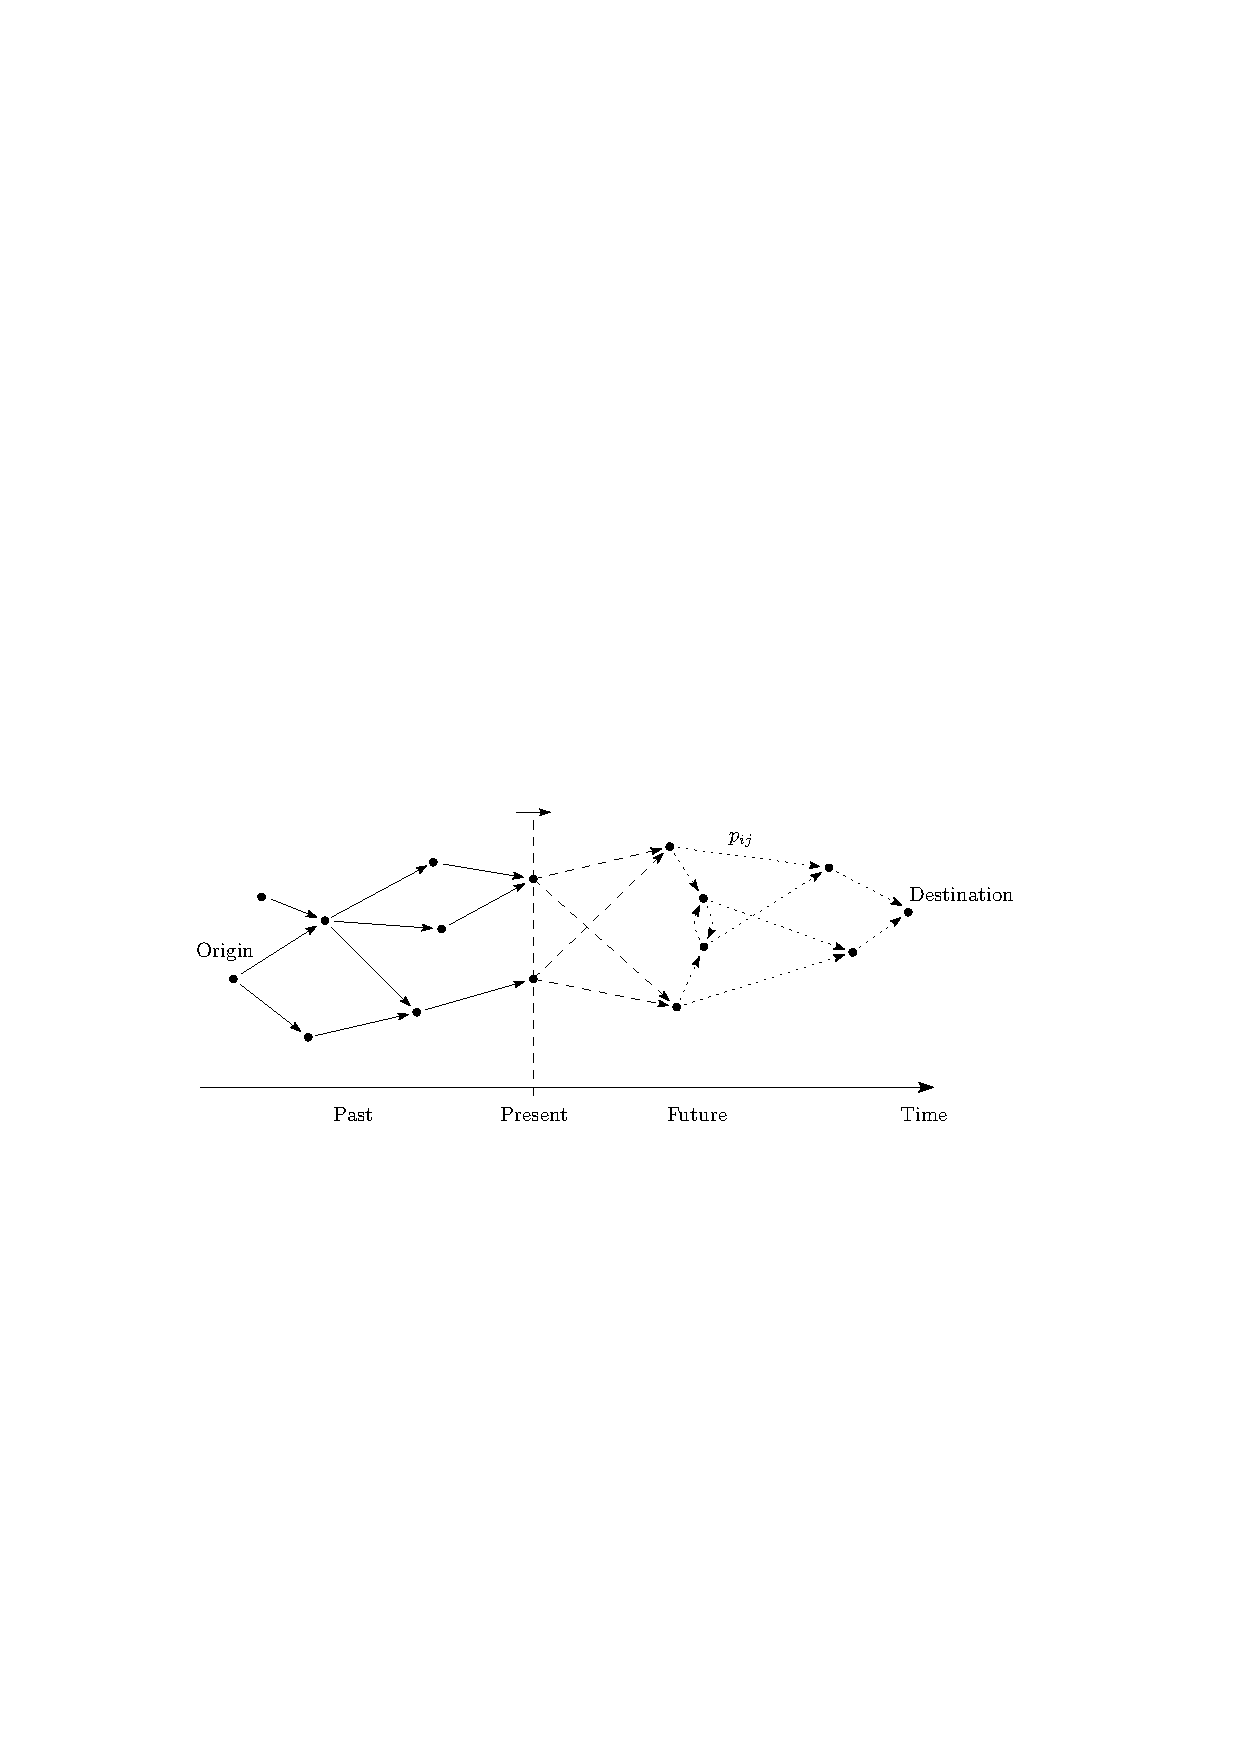
\includegraphics[width=0.9\textwidth]{randomgraph}
\end{center}
\caption{A timeline of the history independent markov decision process. The points denote states (=legs) and the arrows
between the points denote transfers between states. The solid arrows denote
successful \emph{past transfers}, which
form an acyclic graph. The dashed arrows denote \emph{present transfers}, which are realized
at the present time. The dotted arrows denote \emph{future transfers} $i\to j$, each
of which is successful with prior probability $p_{ij}$. Note that there may exist 
states $i,j$ for which both $p_{ij}>0$ and $p_{ji}>0$. Over time, 
future transfers become present transfers and present transfers become
past transfers.
}
\label{randomgraph}
\end{figure}


We suggest that the history independent model \eqref{rekursio02} can be used to
approximate the conditional case \eqref{statejoukko}.
The following theorem characterizes the relation between the two models.
\begin{theorem}
\label{durationthm}
Let $i,j$ and $k$ denote three legs and
let $D_j$ denote the random duration of leg $j$.
Given that the transfer $i \to j$ is successful and assuming that the durations of 
legs are independent, the conditional probability 
$P(\tau_{j}' \leq \tau_{k} \ | \ \tau_{i}' \leq \tau_{j})$ of a successful
transfer $j \to k$ satisfies
\begin{align*}
P(\tau_{j}' \leq \tau_{k}) \geq 
P(\tau_{j}' \leq \tau_{k} \ | \ \tau_{i}' \leq \tau_{j}) \geq 
\frac{P(\tau_{i}' \leq \textnormal{inf supp} f_{\tau_{j}})}{P(\tau_{i}' \leq \tau_{j})} P(\tau_{j}' \leq \tau_{k}), 
\end{align*}
where $\textnormal{inf supp} f_{\tau_{j}}$ denotes the greatest real number $t$ for which $f_{\tau_j}(t) = 0$ and
$t \leq x$ for all $x$ satisfying $f_{\tau_j}(x) > 0$.
\end{theorem}
Theorem \ref{durationthm} states that if the distributions of $\tau_i'$ and $\tau_j$ are
relatively far apart, the conditional probability $P(\tau_{j}' \leq \tau_{k} \ | \ \tau_{i}' \leq \tau_{j})$
of a successful transfer from $j$ to $k$ is close to the unconditional probability $P(\tau_{j}' \leq \tau_{k})$.
In this case, the two leg duration models discussed above converge and the 
independent durations model can be approximated by assuming independence of start and end times. 




\subsection{Unconditional transfers}
\label{unconditional}
The history independent model defined by Equation \eqref{rekursio02} can be further approximated by 
assuming that successful transfers from a state $s$ to its successor states are 
independent events, which is not generally true. However, if the 
spreads of the time distributions are relatively small, we obtain a 
reasonable approximation by assuming independence of successful transfers. 
From a practical viewpoint, since we are particularly interested in the choice for the commuter in 
each situation, the values 
are not as interesting  as the \emph{descending order} of the values, that is, the action at each state.
We suggest that even if approximate models are used, the actions of 
the commuter are in most cases similar as with more accurate models since the 
descending order of the probabilities is preserved.

Since transfers between legs are assumed to be independent events, the transition probability function \eqref{ekakaava} satisfies
\begin{align}
\label{ylaraja01}
P_a(s,s^{a,k}) 
= 
P\left(\tau_{s}' \leq \tau_{s^{a,k}} \cap \bigcap_{g=1}^{k-1} \tau_{s}' > \tau_{s^{a,g}} \right)
= \sum_{k=1}^h p_{ss^{a,k}} \prod_{g = 1}^{k-1}(1-p_{ss^{a,g}}),
\end{align}
where $p_{ss^{a,k}}$ denotes the prior transfer probability from $s$ to $s^{a,k}$, as defined in Equation \eqref{transferprob}.

\begin{theorem}
The history independent value $V_H(s)$ defined by model \eqref{rekursio02} and the unconditional value $V_U(s)$ 
defined by \eqref{ylaraja01} satisfy $V_H(s) \leq V_U(s)$ for all $s \in \{1,\ldots,n\}$.
\end{theorem} 
Note in particular that if the transfer probabilities satisfy $P(\tau_{s}' \leq \tau_{s^{a,k}}) \in \{0,1\}$
for all successor states $s^{a,k} \in S_{s}$, we have $V_H(s) = V_U(s) = V_U(s^{a,k^*})$, where $k^*$ is the smallest index 
for which $P(\tau_{s}' \leq \tau_{s^{a,k}}) = 1$. In this case, the history independent and unconditional
coincide. In other words, the approximation given by \eqref{ylaraja01} is seen to be most accurate when 
the variances of the arrival times are small, which means that the transfer probabilities are likely
to be close to zero or one. 

Furthermore, if each state has a single successor state, the history independent and unconditional models yield the same result.
We suggest that the accuracy of the unconditional model is greatest when the average number of successor states is small.

\subsection{Expected number of successful paths [\ref{jtoits}]}
\label{enumber}
\ref{jtoits} presents the following approximate method for maximizing the reliability
of a journey from
the origin leg $1$ to the destination leg $n$ in the unconditional model described in the previous
section. The approach is to maximize the \emph{expected number 
of successful paths} to the destination leg from each leg of the journey. 
The method is motivated by the idea that paths that allow several detours are considered
more reliable than paths with no alternatives (see Figure \ref{stokvsdet01}).

Let $h_i$ denote the expected number of successful acyclic paths from leg $i \in \{1,\ldots,n-1\}$ 
to the destination leg $n$. When the commuter is
at leg $i$, the available transfer options $X$ to successor legs are revealed. 
The commuter transfers to the leg $i' \in X$ for which $h_{i'}$ is maximized.

Theorem \ref{epolut} establishes a relation between eigenvectors and the expected number of successful paths.
For this purpose, we define a \emph{sink graph} as follows.
\begin{definition}
  Let $G=(V,A)$ be a weighted directed acyclic graph, where a weight $p_{ij} \in [0,1]$ is assigned to each arc $(i,j) \in A$
and let $s \in V$ be a node such that $(s,i) \notin A$ for all $i \in V$.
The graph $G_s=(V, A \cup (s,s))$, where $p_{ss}=1$, is called a \emph{sink graph}. 
\end{definition}
In other words, a sink graph is a weighted directed acyclic graph $(V,A)$ with the exception that one node $s \in V$ with zero outdegree is
associated with a loop $(s,s)$.

\begin{theorem}
\label{epolut}
Let $P$ denote the adjacency matrix of a sink graph $G_s=(V,A)$, where $V=\{1,\ldots,|V|\}$,  
let $h_i$ denote the expected number of successful paths from $i$ to $s$ for $i \in V \setminus \{s\}$ and let $h_s=1$. 
Then, $h=(h_1,\ldots,h_{|V|})^T$ is a unique dominant eigenvector of $L$.
\end{theorem}
Theorem \ref{epolut} states that by constructing a sink graph, the expected number of successful paths $h_i$ from leg $i$ to the destination leg $n$
is given by the dominant eigenvector of the adjacency matrix $P$ consisting of the prior transfer probabilities $p_{ij}$
between legs (and $p_{nn}=1$). 

The expected number of successful paths can also be calculated for all legs that are reachable from the 
origin leg by means of Algorithm \ref{backward02}.
\begin{algorithm}
\begin{algorithmic}
\IF {$h_i \geq 0$ \ \ ($h_i$ has already been determined )}
\STATE Return $h_i$;
\ENDIF
\FORALL {$i' \in S_{i} $ such that $p_{ij} > 0$ ($S_i$ = successor set of $i$)}
\STATE $h_{i'} \leftarrow $ Ex($i'$); 
\ENDFOR
\STATE $h_i \leftarrow \sum_{j \in S_i} p_{ij} h_j$;
\STATE Return $h_i$;
\end{algorithmic}
\caption{A recursive function Ex($i$) for calculating the expected number of feasible 
paths $h_i$ from leg $i$ to the destination leg $n$. 
Initially, set $h_i=-1$ for all $i \in \{1,\ldots,n-1\}$ and $h_n \leftarrow 1$.}
\label{backward02}
\end{algorithm}
The complexity of the algorithm is of order $\mathcal{O}(n+|A|)$, where $A$ is the set of transfers for which $p_{ij} > 0$.
Letting $m = \max_{i \in \{1,\ldots,n-1\}} |S_i|$ denote size of the largest successor set, the complexity
is bounded above by $\mathcal{O}(n(m+1))$.




\section{Numerical experiments}
\label{experiments}
In the following, we present computational results obtained by the 
conditional model \eqref{statejoukko} and the unconditional model \eqref{ylaraja01}.
In the conditional model, the durations of legs are assumed to be independent 
and in the unconditional model, the start and end times of legs are assumed to
be independent, as described in Section \ref{independentstartandendtimes}.
The studied instances are based on the tram network of Helsinki, see Figure \ref{verkot01}.

\begin{figure}[ht]
\begin{center}
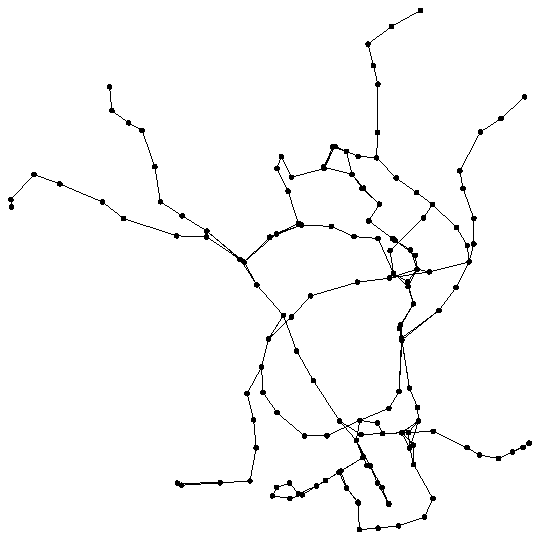
\includegraphics[width=0.7\columnwidth]{verkot01a}
\end{center}
\caption{The tram network of Helsinki consisting of ten tram lines and 154 stops. 
}
\label{verkot01}
\end{figure}

The travel times between stops are defined as shifted gamma distributed random variables. 
More precisely, given the average travel time $t_{uv}$ between stops $u$ and $v$, we define the 
travel time $\tau_{uv}$ as a random variable $\tau_{uv} \sim \text{Gamma}( \alpha t_{uv}, \beta , \delta t_{uv} )$,
where the $\text{Gamma}( \alpha, \beta , \delta )$ distribution is defined by the 
probability density function 
\begin{align}
\label{gammakaava}
f(x)=\frac{(x-\delta)^{\alpha-1} e^{-(x-\delta)/\beta}}{\beta^{\alpha} \Gamma (\alpha)} \ \ \ \mbox{ for } x > \delta \geq 0.
\end{align}
The mean of a $\text{Gamma} (\alpha, \beta, \delta)$ distribution is $\alpha \beta + \delta$,
that is, by choosing $\alpha, \beta$ and $\delta$ such that $\alpha \beta + \delta= 1$,
we have $E(\tau_{uv})=t_{uv}$. 


\subsection{Results}
\begin{table}[ht] 
\caption{Computational results of the conditional and unconditional models, 99.9\% screening. 
The decision time for each model is given by the sum of screening time and algorithm time.}
\centering     
{\tiny
\begin{tabular}{|c|c|c|c|cc|cc|}
\hline 
\multirow{2}{*}{Instance} & Number &Time horizon & Screening  & \multicolumn{2}{|c|}{Conditional model } & 
\multicolumn{2}{|c|}{Unconditional model}\\
\cline{5-8}
& of legs & $T$ (min) & time (s) & Algorithm time (s) & Probability $V((1))$ & Algorithm time (s) & Probability $V_U(1)$ \\
\hline 
 \text{r1} & 745 & 20.4 & 455.29 & 12.42 & 0.989 &  0.54 & 0.989 \\
 \text{r2} & 559 & 18. & 474.83 & 62.67 & 0.693 & 3.99 & 0.693 \\
 \text{r3} & 90 & 9.6 & 36.33 & 4.15 & 0.482 & 0.14 & 0.504 \\
 \text{r4} & 355 & 15.6 & 1419.24 & 898.54 & 0.839 &  2.08 & 0.859 \\
 \text{r5} & 558 & 24. & 234.2 & 5.94 & 0.181  & 0.28 & 0.203 \\
 \text{r6} & 704 & 22.8 & 1646.43 & 98.31 & 0.677  & 3.04 & 0.678 \\
 \text{r7} & 615 & 19.2 & 1642.85 & 30.05 & 0.555  & 2.66 & 0.602 \\
 \text{r8} & 562 & 21.6 & 1028.88 & 20.94 & 0.295  & 1.08 & 0.455 \\
 \text{r9} & 508 & 15.6 & 787.51 & 883.16 & 0.588  & 1.43 & 0.677 \\
 \text{r10} & 85 & 10.8 & 37.57 & 4.64 & 0.311 & 0.49 & 0.312 \\
 \hline
\end{tabular}
}
\label{tulokset01a}
\end{table}


The computational results are shown in Table \ref{tulokset01a}, 
The first column shows the name of the instance, the second column shows the number of
legs included the instance and the third column shows the length of the time window in minutes.

In order to be able to compute the probability in the conditional model, 
which requires the enumeration of all paths,
the set of paths from the origin state to destination states was initially narrowed by excluding paths for
which the probability of success is less than a minimum probability $p$ with confidence level $1-p$.
The duration of this screening phase (in seconds) is shown in the third column of the tables.

The remaining columns show the algorithm times for the different models and the corresponding probability values for the 
origin state. The \emph{decision time} for each model is given by the sum of screening time and algorithm time.
The decision time corresponds to the time needed to produce an optimal policy in each instance, that is, 
the time needed to suggest a decision for the commuter.

In the screening phase, paths for
which the probability of success is less than 0.1\% with a 99.9\% confidence level were excluded.
This screening phase was executed by performing $R=6905$ random tests, in each of which all paths
beginning from the origin state were enumerated.
For all states not excluded during the screening phase, the distributions of the start and end times in the conditional model were 
approximated by random sampling with $R=10000$ samples.

By looking at the algorithm times in the tables,  
we see that the unconditional algorithm is significantly, typically of order ten times, faster than the  conditional model.
Furthermore, in a part of the instances, the difference between the results obtained by the 
models is insignificant. For example, in instance r6, the probability of reaching the destination state
is equal with three-digit precision for both models.
However, the results also indicate that the modeling error in the unconditional model is significant in some cases. 

As a conclusion, it can be stated that even though the algorithm time of the conditional model is significantly greater 
compared to the unconditional model, the conditional model is justified by the fact that it may be used to
estimate the error in approximate methods. By heuristic screening, the compuation times can be significantly
decreased, see \ref{jdjuejor}.

\chapter{Economic models}
\label{economicmodels}
This chapter presents economic models for demand-responsive transport services, in which customers request trips from specified origins to specified destinations and a fleet of vehicles serves the customers. Customers seek rides to minimize travel time and transport operators aim to maximize profit. 
Demand-responsive transport is considered as a complementary service to conventional public transport services and 
customers are assumed to choose the utility-maximizing alternative from the available transport modes.
An \emph{economic equilibrium} is defined as a state in which the demand meets the supply of trips: 
the choices of transport operators
do not change if the demand remains constant and the choices of customers
do not change if the supply of trips remains constant. 

In Section \ref{networkmodel}, a stochastic model for studying demand-responsive transport services is presented.
Section \ref{simulationmodel} presents a more detailed model based on microsimulation.

\section{Stochastic model [\ref{ccompejor}]}
\label{networkmodel}
\ref{ccompejor} introduces a stochastic network model to characterize the 
behavior of customers and transport operators in a demand-responsive transport market.
The transport operators seek to maximize profit by serving as many customers per unit time as possible, 
and customers seek rides to minimize subjective trip price, defined as a combination of ticket price and travel time. 
Given these behavior models,
we calculate the \emph{network equilibrium}, defined as a state in which the demand matches the supply
of trips in each part of the network. 

This approach is somewhat similar to the taxi model proposed by \cite{yang2010}. The main difference is that in a taxi service, 
customers are delivered to their destinations directly, whereas in a demand-responsive transport service, a vehicle can serve several customers 
simultaneously and therefore a customer's trip from an origin to a destination is not necessarily a direct one. 

The stochastic model for demand-responsive transport is governed by the following preliminary assumptions.
\begin{enumerate}
\item
There are $N$ vehicles that produce trips between 
origins and destinations in a specific operating zone. 
Different trips may have different prices and
travel times. A single vehicle can simultaneously serve several customers.
\item
The subjective price of a trip is defined as a combination of ticket price and travel time.
Customers choose between trips provided by 
DRT and a virtual mode by comparing the subjective 
prices of different trips.
\item
Customers are assigned to vehicles by means of an electronic booking service.
For analysis, we assume that the DRT customers that 
choose trip $r$ are divided equally among vehicles that produce trip $r$. 
\end{enumerate} 
In the following, the behavior of customers (Section \ref{demand}) and transport operators providing service 
(Section \ref{vehiclemovements}) is studied in more detail.

\subsection{Demand}
\label{demand}
Let us consider a set of \emph{nodes} $I$ representing the origins and destinations of customers in a specific operating zone.
Each pair of nodes $(i,j) \in I \times I$ is associated with a specific \emph{direct ride time} $t_{ij}$.

A \emph{trip} from an origin $i_0 \in I$ to a destination $i_d \in I$ is defined as an acyclic sequence of nodes 
$(i_0,i_1,\ldots,i_{d-1},i_d)$ in $I$.
When a customer takes a trip $(i_0,i_1,\ldots,i_{d-1},i_d)$, the customer enters a vehicle at $i_0$, which
visits the nodes $i_1,\ldots,i_{d-1}$ before the drop-off of the customer at $i_d$. That is, the
trip denotes the path of the vehicle that transports the customer from $i_0$ to $i_d$.
For example, a \emph{direct} trip from $i_0 \in I$ to $i_d \in I$, denoted by $(i_0,i_d)$, describes a trip in which a customer enters 
a vehicle at $i_0$ and the vehicle drives directly to $i_d$ without stopping between $i_0$ and $i_d$. 
The set of all trips in $I$ is denoted by $\mathcal{R}$ and the set of trips from $i\in I$ to $j \in I$ is denoted by $\mathcal{R}_{ij}$.

\subsubsection{Subjective price}
Each trip $r \in \mathcal{R}$ has a specific ticket price $p_r$. 
Note that the prices of trips with the same origin and destination may be different.
Similarly as in \citep{yang2010}, each customer seeks a trip to minimize the \emph{subjective price}, 
defined as a combination of $p_r$ and \emph{travel time}. 

The \emph{ride time} of a trip $(i_0,\ldots,i_d) \in \mathcal{R}_{i_0i_d}$ 
refers to the time spent inside a vehicle and is defined by
\begin{align}
\label{ridetime}
q_{(i_0,\ldots,i_d)}^{\rm DRT} = \sum_{k=1}^{d} t_{i_{k-1}i_{k}}.
\end{align}
The ride time from $i_0$ to $i_d$ is minimized in the direct trip $(i_0,i_d)$. 

For any pair of nodes $i,j \in I$,
the demand responsive transport service produces different trips from $i$ to $j$ at different intervals.
That is, there may be different \emph{waiting times} for different trips
(see Section \ref{averagetraveltime} for a more detailed discussion on waiting times).

The average \emph{travel time} for a trip $r \in \mathcal{R}_{ij}$ is defined as
the sum of waiting time and ride time, that is, 
\begin{align}
\label{traveltime}
t_{r}^{\rm DRT} = w_{r}^{\rm DRT} + q_{r}^{\rm DRT}.
\end{align}

%Assuming that the level of service is determined by the average travel time,
The \emph{subjective price} of a DRT trip $r \in \mathcal{R}_{ij}$ is given by
\begin{align}
\label{asiakashinta}
g_{r}^{\rm DRT} = p_{r} + \beta t_{r}^{\rm DRT},
\end{align}
where $p_{r}$ is the ticket price for the trip $r$ and $\beta$ is the customers' 
monetary value of unit travel time. 

%For analysis, we use the notation $p_r = p_{ij}$ for all $r \in \mathcal{R}_{ij}$.
\subsubsection{Demand for DRT}
The choices of customers are determined by a logit model, similar to the one in \citep{yang2010}, as follows.
The subjective trip price of a trip from $i$ to $j$ provided by the \emph{virtual mode}\footnote{The virtual mode 
represents alternatives for the DRT service.} is denoted by $\bar{g}_{ij}$.
The probability that a customer traveling from $i$ to $j$ chooses a DRT trip $r \in \mathcal{R}_{ij}$ is defined by
\begin{align}
\label{kysyntatn}
P_{r}^{\rm DRT} = 
\frac{\exp(-\theta g_{r}^{\rm DRT})}{\exp(-\theta \bar{g}_{ij}) + \sum_{r' \in \mathcal{R}_{ij}}\exp(-\theta g_{r'}^{\rm DRT})},
\end{align}
where $\theta$ is a nonnegative parameter describing the uncertainty in transport services and demand
from the perspective of customers.  
Clearly, the above logit model has the property of independence from irrelevant alternatives, that is, 
the ratio $P_{r}/P_{r'}$ depends on the subjective prices of trips $r$ and $r'$ but
not on the subjective prices of other trips \citep{small2007}.
 

The \emph{total demand} from $i$ to $j$ is denoted by $Q_{ij}$ and describes
the number of customers willing to travel from $i$ to $j$ per unit time.
The corresponding demand for a trip $r \in \mathcal{R}_{ij}$ is given by
\begin{align}
\label{matkakysynta}
Q_{r}^{\rm DRT} = Q_{ij} P_{r}^{\rm DRT}.
\end{align}
The \emph{demand for DRT} describing the expected number of customers that 
choose to travel from $i$ to $j$ by DRT per unit time is given by
\begin{align}
\label{drtkysynta}
Q_{ij}^{\rm DRT} = \sum_{r\in \mathcal{R}_{ij}} Q_{r}^{\rm DRT}.
\end{align}

\subsection{Supply}
\label{vehiclemovements}
We assume that there are $N$ vehicles available for transporting customers. 
At any point in time, each vehicle follows a specific \emph{route} $(i_0,i_1,\ldots,i_m)$ 
determined by a sequence of nodes in the transportation network.
The vehicle starts at the first node $i_0$ and proceeds by visiting the other nodes $i_k$
for $k=1,\ldots,m$ in the order determined by the route.
Each node corresponds to a stop during which customers may enter or exit the vehicle.
We assume that each route is acyclic and consists of a minimum of two nodes, that is, none of the
vehicles are idle at any time. Since the routes are acyclic, each route consists of
a maximum of $|I|$ nodes.

The total time needed to complete a route is given by 
\begin{align}
\label{totaltime}
d_{(i_0,i_1,\ldots,i_m)}^{\rm route} = \sum_{h=1}^m t_{i_{h-1} i_h}
\end{align}
and the total cost of a route equals 
\begin{align}
\label{totalcost}
c_{(i_0,i_1,\ldots,i_m)}^{\rm route} = \sum_{h=1}^m c_{i_{h-1} i_h},
\end{align}
where $c_{i_{h-1}i_h}$ is the cost associated with leg $(i_{h-1},i_h)$.


\subsubsection{Trip production}
When a vehicle following a route $(i_0,i_1,\ldots,i_m)$ arrives at stop $i_k$, customers waiting at $i_k$ to
be transported to any of the stops $i_{k+1},\ldots,i_m$ may enter the vehicle.
In other words, we say that the vehicle \emph{produces} trips from $i_k$ to the nodes $i_{k+1},\ldots,i_m$, see Figure \ref{esim02}.
Formally, the set of produced trips from the current stop $i_k$ to the remaining stops $i_{k+1},\ldots,i_m$ is given by
\begin{align}
\label{tripproduction}
\mathcal{R}_{(i_k,\ldots, i_m)} = \bigcup_{h =k+1}^m \{(i_k,i_{k+1},\ldots,i_h)\}.  
\end{align}


During the execution of the route $(i_0,i_1,\ldots,i_m)$, the vehicle consecutively arrives at stops $i_k$,
where $k=0,\ldots,m$. 
The set of produced trips during the execution of the route equals
\begin{align}
\label{routeproduction}
\mathcal{R}_{(i_0,\ldots, i_m)}^{\rm route} = \bigcup_{k =0}^{m-1} \mathcal{R}_{(i_k,\ldots, i_m)},
\end{align}
that is, the set of subsequences of $(i_0,\ldots, i_m)$. This idea of producing trips 
is in fact similar as in traditional public transport: a bus with a given route 
produces trips that are subsequences of the route (see Figure \ref{esim02}).

\begin{figure}[ht]
\begin{center}
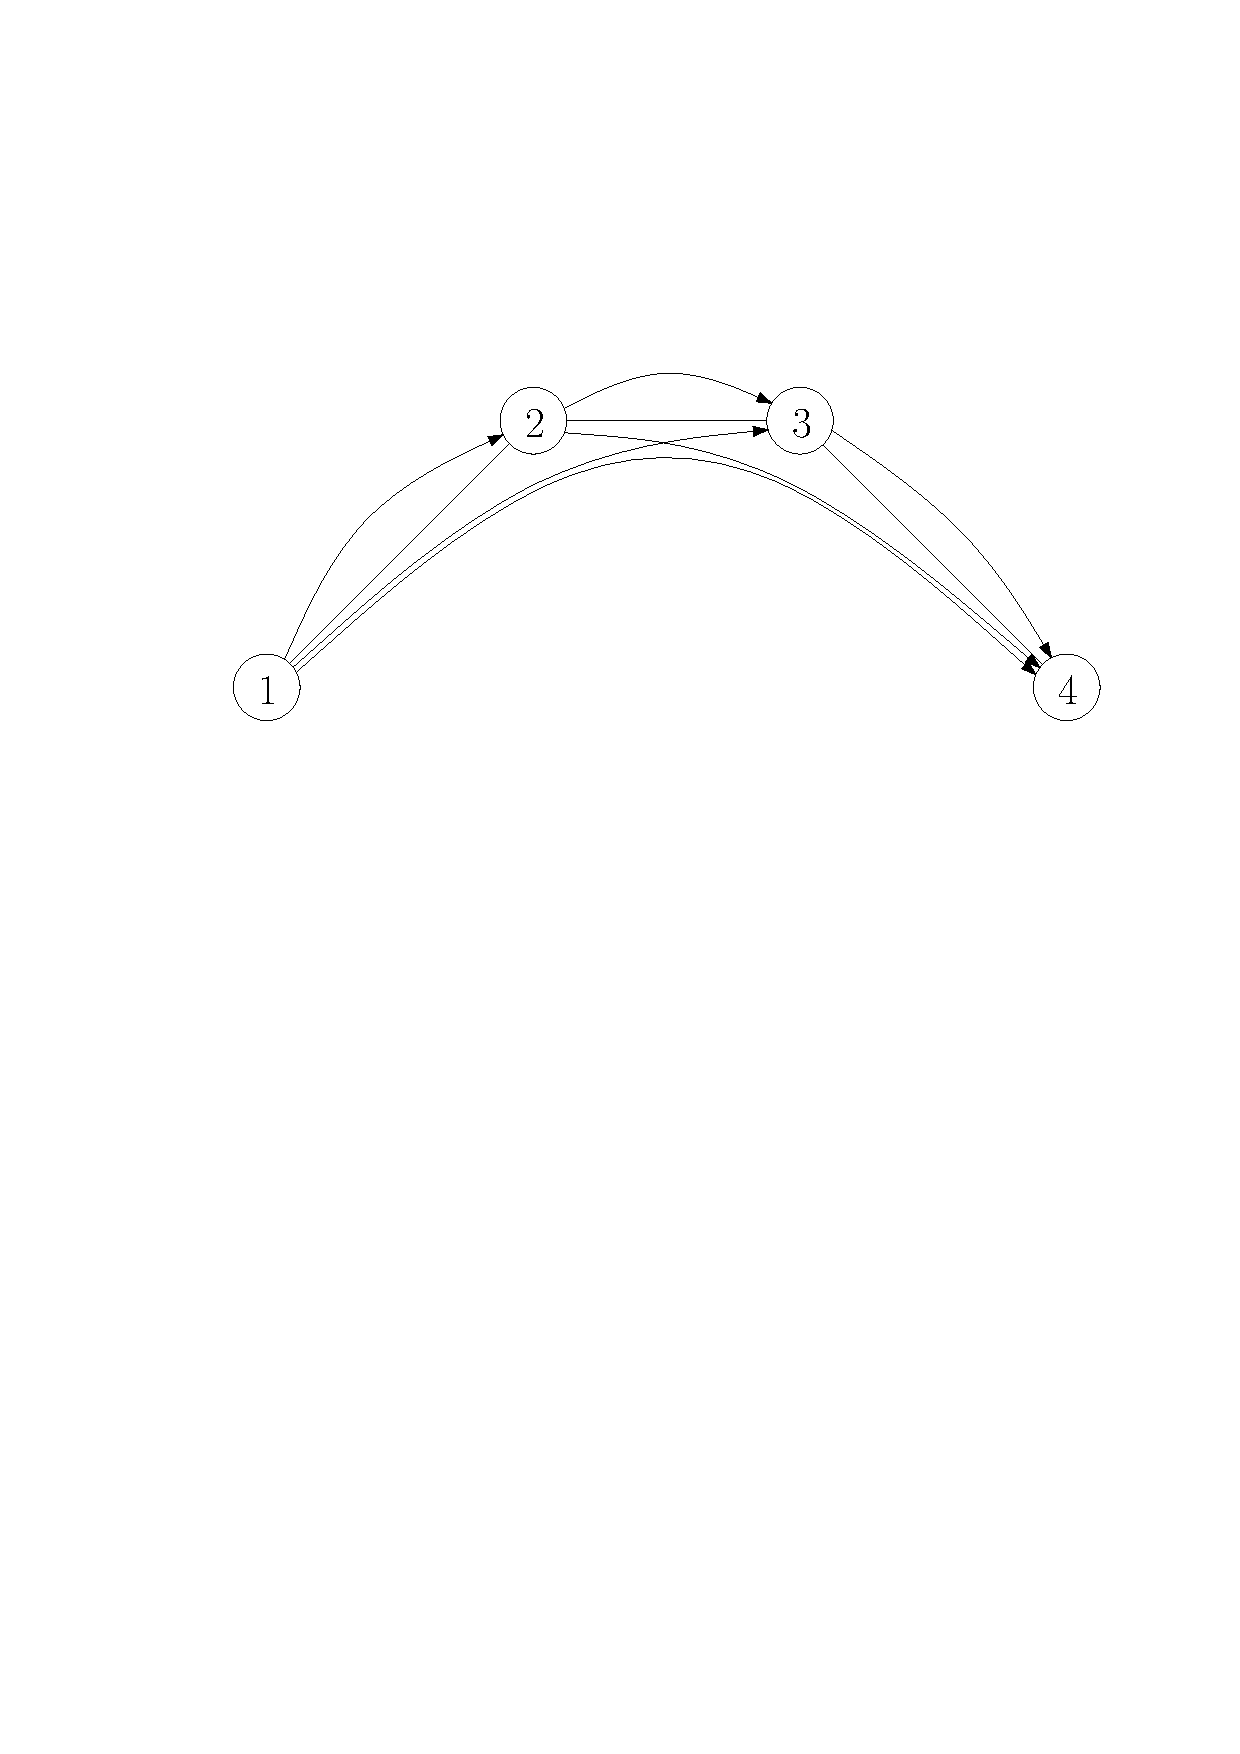
\includegraphics[width=0.7\columnwidth]{esim02}
\caption{Trip production. A vehicle follows the route $(1,2,3,4)$. Upon arrival at each stop, the
vehicle produces trips to the other stops on the route. The
set of produced trips during the execution of the route is equal to the set of subsequences of $(1,2,3,4)$, that is, 
$\mathcal{R}_{(1,2,3,4)}^{\rm route} = \{(1,2),(1,2,3),(1,2,3,4),(2,3),(2,3,4),(3,4)\}$.
}
\label{esim02}
\end{center}
\end{figure}


\subsubsection{Route modifications}
\label{routemodifications}
The most distinguishing feature of demand-responsive transport, which differentiates it from 
traditional public transport, is that the vehicle routes may be modified in
real time in order to meet the demand for transportation efficiently.
\ref{ccompejor} considers the following type of route modifications.

Suppose a vehicle follows a route $(i_0,\ldots,i_m)$ and arrives at node $i_k$.
Naturally, the vehicle produces trips from $i_k$ to all remaining nodes $i_{k+1},\ldots,i_m$.
In order to serve additional customers, the route may be
\emph{extended} by adding a sequence of nodes $i_{m+1},\ldots,i_q$ to 
the end of the route (see Figure \ref{esim01}). In this case, the vehicle produces the set of trips 
$\mathcal{R}_{(i_k,\ldots, i_q)}$
from $i_k$ to the stops $(i_{k+1},\ldots,i_q)$, see Figure \ref{esim01}c.

When a vehicle following a route $(i_0,\ldots,i_m)$ arrives at $i_k$, where $0 \leq k < m$, there
are two options:
\begin{itemize}
\item
The route is \emph{extended}. The vehicle transfers to a new route beginning at $i_k$, namely, $(i_{k},\ldots,i_q)$.
\item
The route is \emph{not extended}. The vehicle proceeds by executing the current route $(i_0,\ldots,i_m)$.
\end{itemize}
By definition, the minimum number of nodes in a route is two. Thus, when the vehicle arrives at $i_m$,
the route is automatically extended.


\begin{figure}[ht]
\begin{center}
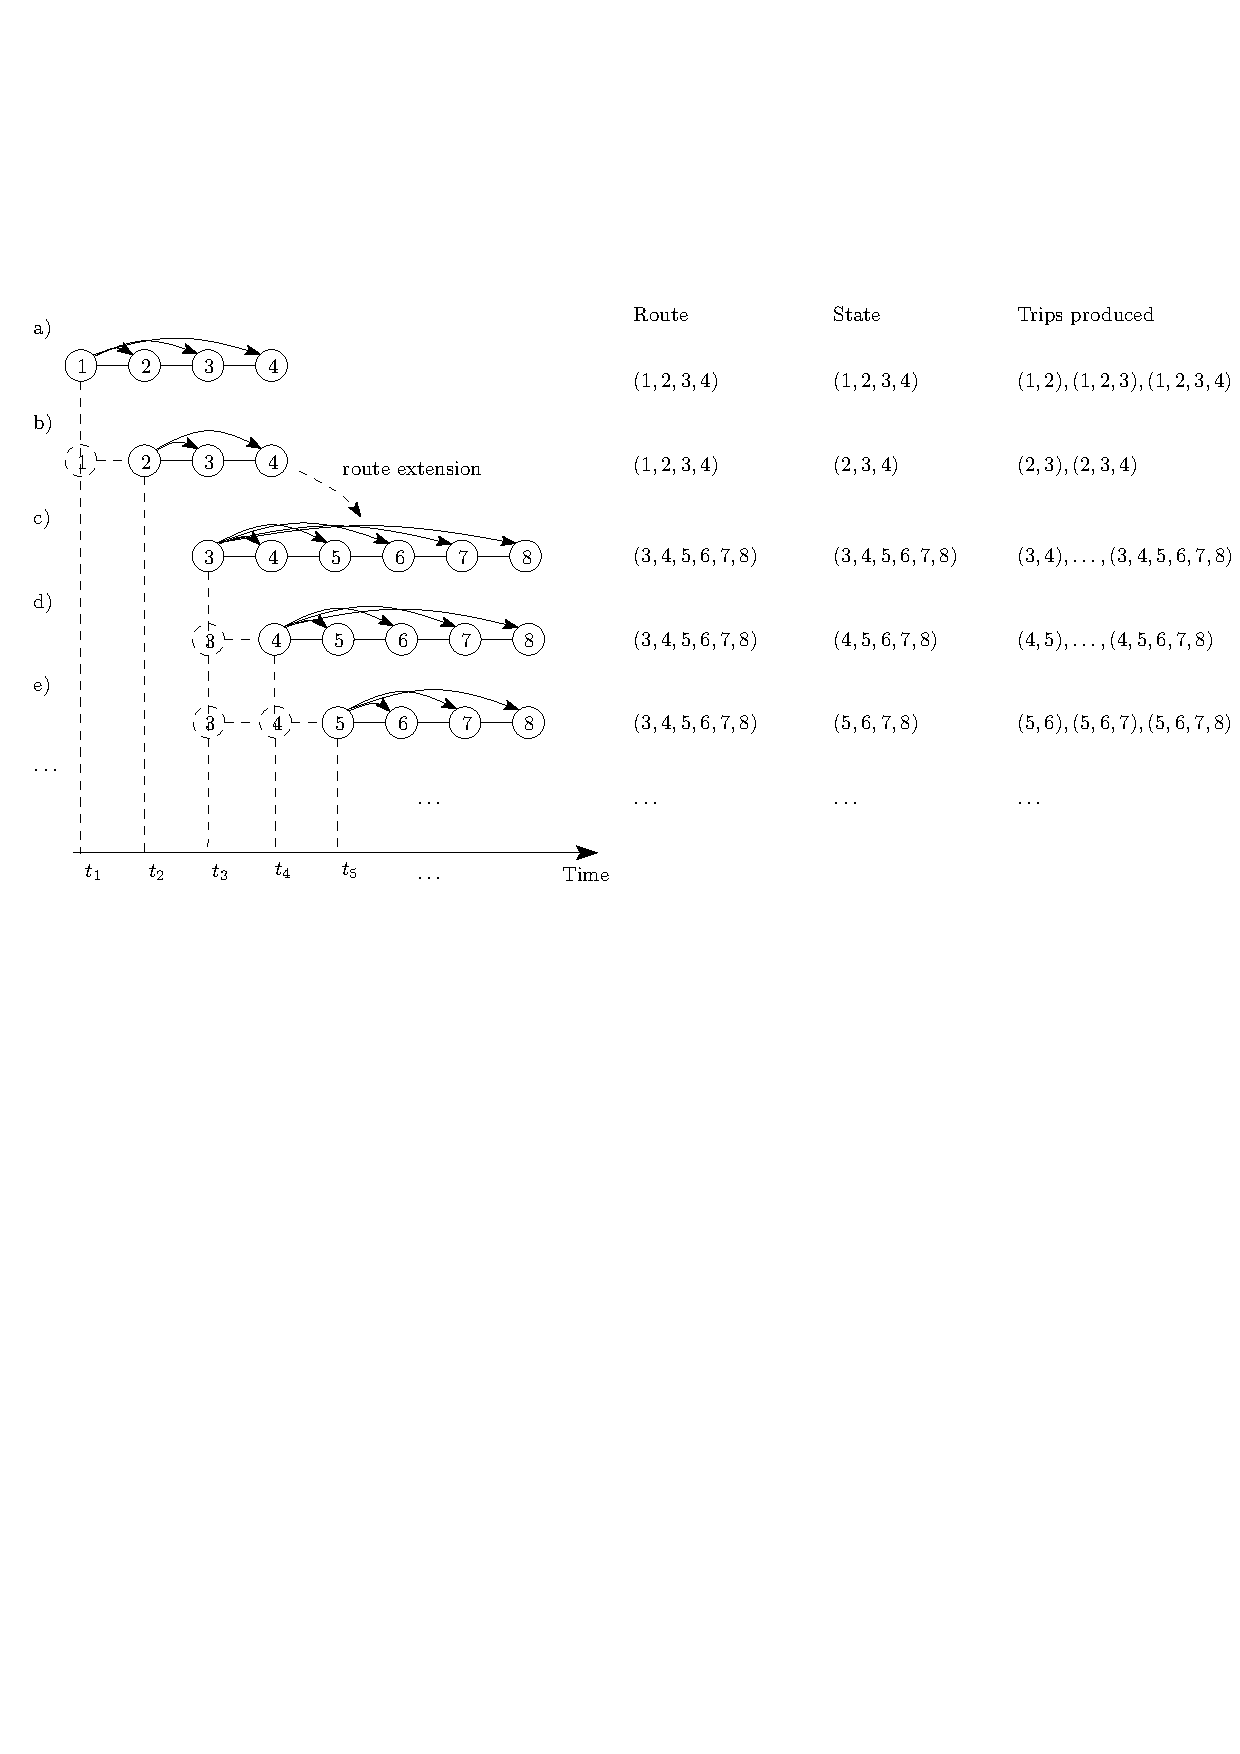
\includegraphics[width=1.0\columnwidth]{esim01}
\caption{Routes, states and trips. a) At $t_1$, a vehicle follows the route $(1,2,3,4)$ consisting
of four nodes. Customers are transported from $1$ to $2,3$ and $4$. b) At time $t_2$, the 
vehicle arrives at node $2$. At this instant, customers waiting at $2$ to be transported to $3$ or $4$ may enter the vehicle, that is, the vehicle 
produces trips $(2,3)$ and $(2,3,4)$. The route of the vehicle remains unchanged. c)
At $t_3$, the vehicle arrives at node $3$. In addition to node $4$, the driver chooses to offer transportation from node $3$ to nodes 
$5,\ldots,8$. In this case, the vehicle produces trips $(3,4),(3,4,5),(3,4,5,6),(3,4,5,6,7),(3,4,5,6,7,8)$.
The route of the vehicle is extended, and the new route is $(3,4,5,6,7,8)$. The execution of the
new route is represented as a sequence of states, namely $(3,4,5,6,7,8), (4,5,6,7,8), \ldots, (7,8)$,
see Figures c,d,e.
}
\label{esim01}
\end{center}
\end{figure}

In the following, the route extensions and production of trips is discussed in more detail
by representing routes as sequences of \emph{states}.


\subsubsection{States}
The \emph{state} of a vehicle describes which part of the route the vehicle is currently executing.
Each time a vehicle following a route $(i_0,\ldots,i_m)$ arrives at stop $i_k$, 
we say that the vehicle \emph{transfers} to a new state.
Similarly as routes, the states are defined as sequences of nodes.
The difference between states and routes
is that the state of a vehicle corresponds to the \emph{remaining part} of its current route. 
That is, the vehicle transfers to a new state each time it arrives at a stop, even if the route remains unchanged.
During the execution of a route $(i_0,\ldots,i_m)$, the vehicle successively transfers to states 
$(i_0,\ldots,i_m),(i_1,\ldots,i_m),(i_2,\ldots,i_m),\ldots,(i_{m-1},i_m)$.
For example, in Figure \ref{esim01}, the vehicle follows the same route in both \ref{esim01}a and \ref{esim01}b,
but the state in \ref{esim01}a is $(1,2,3,4)$ and the state in \ref{esim01}b is $(2,3,4)$. In \ref{esim01}c,
the vehicle transfers to state $(3,4,5,6,7,8)$.
%defined by the remaining part of the route. 

Generally, the set of states is defined by
\begin{align*}
\mathcal{S} = \{ (i_0,i_1,\ldots, i_m) \ | \ & m \geq 1, \ (h \neq g \Rightarrow i_h \neq i_g), \ i_h,i_g \in I  \mbox{ for all } h,g \in \{0,\ldots,m\} \}.
\end{align*}
The total number of states equals $|\mathcal{S}| = \sum_{l=2}^{|I|} {|I| \choose l} l!$.
Note that the set of states is equal to the set of trips, that is, $\mathcal{S}=\mathcal{R}$.

When a vehicle arrives at a stop, the route of the vehicle may be extended by adding a sequence of nodes to the
end of the route, as dicussed in Section \ref{routemodifications}. In other words, the set of states \emph{to} 
which a transfer from state $s = (i_0,\ldots,i_m)$ is possible is defined by
\begin{align}
\label{successors}
\mathcal{S}_{s} = \{ (s_1,\ldots ,i_m,i_{m+1},\ldots,i_q) \in \mathcal{S} \ | \ i_{m+1},\ldots,i_q \in I \}.
\end{align}
This set will be referred to as the \emph{successor set} of state $s$.
Note that if the route is not extended, we have $q=m$ in the above equation.

The first two nodes $i_0,i_1$ of a state $(i_0,\ldots,i_m)$ determine the leg the vehicle is currently traversing.
Since the state of the vehicle is modified at the time the vehicle arrives at $i_1$, 
the duration of a state $(i_0,\ldots,i_m)$ is given by 
\begin{align}
\label{stateduration}
d_{(i_0,\ldots, i_m)} = t_{i_0i_1}. 
\end{align}
Note that the duration of a state $(i_0,\ldots, i_m)$ is generally different from the total
time \eqref{totaltime} needed to complete the route.

\subsubsection{Arrival rate and production rate}
The \emph{arrival rate} of vehicles at state $s \in \mathcal{S}$ describes the 
number of vehicles arriving at state $s$ per unit time and is denoted by $T_s$.
During a finite time period $[0,t]$, we require that the total service time of vehicles 
at different states equals $Nt$, that is,
\begin{align}
\label{rajoitus01}
\sum_{s \in \mathcal{S}} t T_s d_s = Nt \ \ \ \ 
\Leftrightarrow \ \ \ \ \sum_{s \in \mathcal{S}} T_s d_s = N,
\end{align}
where $d_s$ is the duration of state $s$ defined by Equation \eqref{stateduration}.

Let us consider the \emph{production rate} $T_{r}^p$ for a trip $r \in \mathcal{R}$,
that is, how many times the trip $r$ is produced per unit time.
Using the notation of \eqref{tripproduction}, we note that a state $s$ \emph{produces}
the set of trips $\mathcal{R}_s$, that is, the set of all subsequences of $s$
beginning from the first node of $s$.
Correspondingly, for any trip $r \in \mathcal{R}$, %For any node $i_h$, where $h \in \{2,\ldots,q\}$, 
we define the set of states that produce trip $r$ by 
\begin{align*}
\mathcal{S}_{r}^p = \{ s \in \mathcal{S} \ | \ r \in \mathcal{R}_s \}, 
\end{align*}
where $\mathcal{S}$ is the set of all states. That is, a state $s$ is included in $S_r^p$
if $r$ is a subsequence of $s$ beginning from the first node in $s$.

Thus, the production rate $T_{r}^p$ for a trip $r$
is given by the total arrival rate of vehicles at states $s \in \mathcal{S}_{r}^p$ that 
produce trip $r$, that is,
\begin{align}
\label{totalrate}
T_{r}^p = \sum_{s \in \mathcal{S}_{r}^p} T_s,
\end{align}
where $T_s$ is the arrival rate of vehicles at state $s$ (see Figure \ref{arrivalrates}).

\begin{figure}[ht]
\begin{center}
{\small
\begin{tabular}{c|c|c|c|}
\cline{2-4}
\multirow{6}{*}{
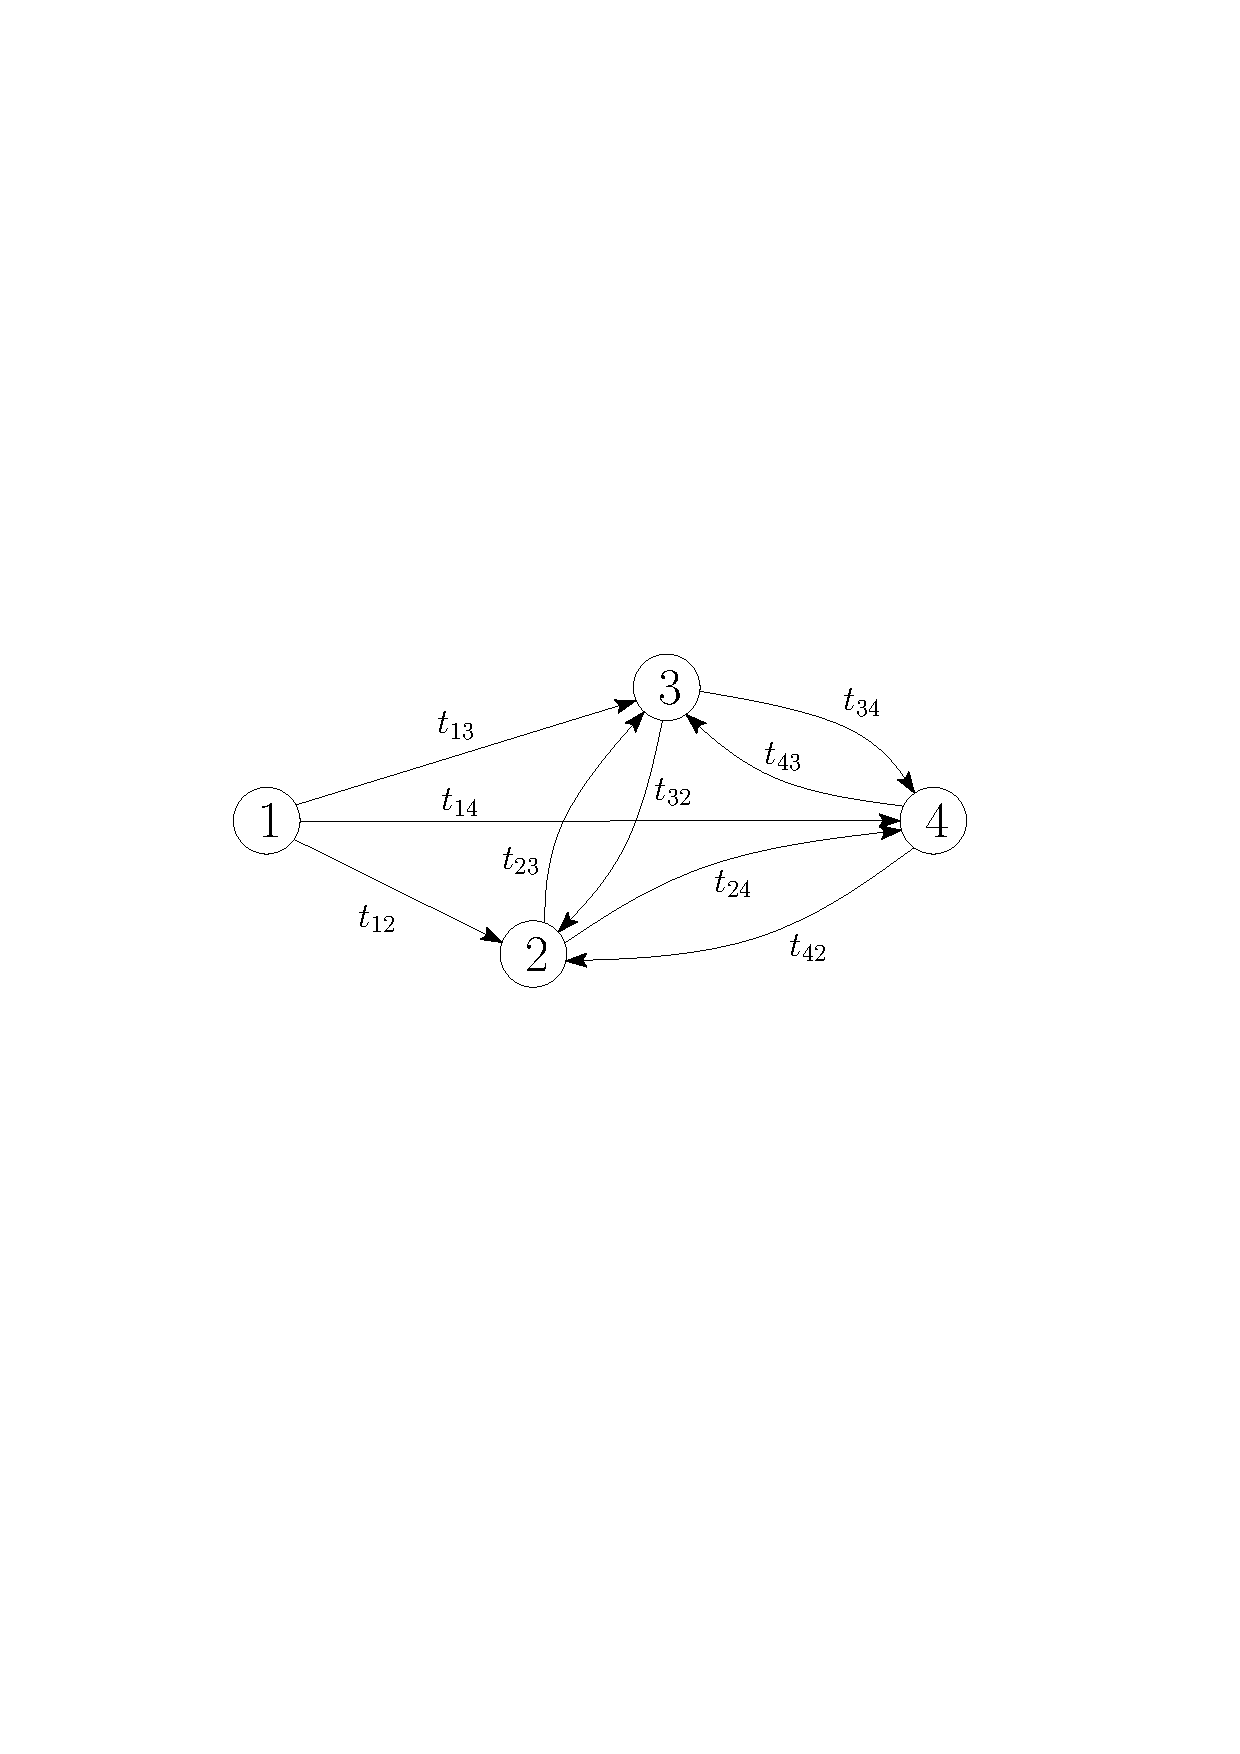
\includegraphics[width=0.35\columnwidth]{arrivalrates} 
} 
& Trip $r \in \mathcal{R}_{14}$ & Ride time $q_{r}$ & States $S_r^p$ that produce $r$ \\
\cline{2-4}
& $(1,4)$ & $t_{14}$ & $(1,4),(1,4,2),(1,4,3), $  \\
&  &   &  $(1,4,2,3),(1,4,3,2)$   \\
\cline{2-4}
& $(1,2,4)$ & $t_{12}+t_{24}$ & $(1,2,4), (1,2,4,3)$ \\
\cline{2-4}
& $(1,3,4)$ & $t_{13}+t_{34}$ & $(1,3,4), (1,3,4,2)$ \\
\cline{2-4}
& $(1,2,3,4)$ & $t_{12}+t_{23} + t_{34}$ & $(1,2,3,4)$ \\
\cline{2-4}
& $(1,3,2,4)$ & $t_{13}+t_{32} + t_{24}$ & $(1,3,2,4)$  \\
\cline{2-4}
\end{tabular}
}
\end{center}
\caption{The production rate for different trips between two nodes. 
Let us consider the rate of vehicles producing trips
from node $1$ to node $4$ in the example network presented in the figure. 
The trips $r \in \mathcal{R}_{14}$ from $1$ to $4$ are presented in the first column of the table next to the figure.
The second column of the table shows the ride time $q_{r}$ for the trip $r$ and the
third column shows the set of states $\mathcal{S}_r^p$ that produce the trip $r$. 
The production rate $T_{r}^p$
for a trip $r$ is defined as the sum of the arrival rates $T_s$ of vehicles at states $s \in \mathcal{S}_r^p$
that produce trip $r$. The average travel time for
a trip $r$ is given by $t_r^{\rm DRT} = \frac{1}{T_r^p} + q_{r}$.
}
\label{arrivalrates}
\end{figure}

\subsubsection{Average travel time}
\label{averagetraveltime}
Let us then consider the \emph{average travel time} $t_{r}^{\rm DRT}$ for a trip $r \in \mathcal{R}$, 
defined as the sum of waiting time and ride time, see Equation \eqref{traveltime}.

The ride time $q_r^{\rm DRT}$ for a trip $r$ is given by Equation \eqref{ridetime}.
The average waiting time $w_r^{\rm DRT}$ for a trip $r$ depends on the production rate $T_r^p$ of the trip, 
that is, the arrival rate of vehicles at states $S_r^p$ that produce trip $r$.

We assume that the vehicles arrive according to a Poisson process, in which 
arrivals occur continuously and independently of one another \citep{ross}.
In this case, the
expected waiting time for a customer departing at a random instant is equal to the expected 
time interval between arrivals, that is, $w_r^{\rm DRT} = \frac {1}{T_{r}^p}$.
The average travel time is thus given by
\begin{align}
\label{ajoaika}
t_{r}^{\rm DRT}= 
\left\{
\begin{array}{ll}
\frac {1}{T_{r}^p} + q_r^{\rm DRT} & \mbox{if } T_{r}^p > 0, \\
\infty & \mbox{otherwise.}
\end{array}
\right.
\end{align}

For instance, if during one hour there are three vehicles that produce a trip $r$ 
for which the \emph{ride time} is 10 minutes, the average \emph{travel time} for that trip
is given by adding the average \emph{waiting time}, that is, $t_{r}^{\rm DRT}= \frac {1}{\frac{3}{60}}  + 10 = 30$ minutes.

Note that if the production rate $T_{r}^p$ for a trip $r \in \mathcal{R}$ is zero, the
average travel time for $r$ is infinite. In this case, the demand for the trip is zero, 
see Equation \eqref{kysyntatn}. 


\subsection{Competitive market}
Most existing demand-responsive transport services provide door-to-door transportation for elderly or handicapped people
and require customers to book trips at least one hour in advance \citep{cordeau05,jouko}.
Conventionally, the trips are organized centrally via \emph{travel dispatch centers}, which have the capability of
assigning customers to vehicles and optimizing the routes \citep{mageean}.
In contrast to such centralized services, \ref{ccompejor} considers a competitive form of demand-responsive transport in which 
each driver providing service attempts to maximize his/her profit. That is,
the movement of vehicles is governed by the decisions of individual drivers, 
instead of a travel dispatch center controlled by a single transport operator.
This market structure is in fact similar to conventional taxi-markets, which have been extensively studied, see for example 
\citep{hackner1995,arnott1996,cairns1996,flores-guri2003,lagos2003,wong2005,matsushima2006,fernandez2006,moore2006,yang2002,yang2005,yang2010}.

In a competitive market, the drivers attempt to transfer to
states at which the \emph{expected profit rate} is maximized. By using the expected profit rate as a 
utility measure we can compare the profitability of routes of different lengths.

Given that a single vehicle arrives at state $s \in \mathcal{S}_{r}^p$ that 
produces a trip $r \in \mathcal{R}_{ij}$ from $i$ to $j$, 
let us study the expected number $E[Q_{r}^1]$ of DRT customers traveling 
from $i$ to $j$ that enter the vehicle.
We determine $E[Q_{r}^1]$ by
dividing the demand $E[Q_{r}^{\rm DRT}]$ for the trip $r$ by the total production rate $T_r^p$ of 
the trip, that is,
\begin{align}
E[Q_{r}^1] = \frac{E[Q_{r}^{\rm DRT}]}{ T_{r}^p}.
\end{align}
This equation is justified by the assumption that the customers
that choose the trip $r$ are divided equally among
vehicles that produce the trip $r$.
For instance, if during one hour there are three vehicles that produce a trip $r$ and the demand
for the trip $r$ is six customers/hour, the expected number of DRT customers
for a single vehicle equals $E[Q_{r}^1] = \frac{6 \ {\rm customers/h}}{3 \ {\rm vehicles/h}} = 2 \ {\rm customers/vehicle}$.

Let us then consider the expected profit rate for a vehicle 
arriving at state $s=(i_1,\ldots,i_m)$. For analysis, the expected profit rate is calculated
by assuming that the 
route corresponding to $s$ is not extended during its execution. 
That is, the vehicle executes the route by successively transferring to 
states $(i_1,\ldots,i_m),(i_2,\ldots,i_m),\ldots,(i_{m-1},i_m)$.
In this case, the    
set of trips produced during the execution equals
$\mathcal{R}_{s}^{\rm route}$ defined by Equation \eqref{routeproduction}, that is, the
set of all subsequences of $s$ (see Figure \ref{esim02}).

The expected number of customers that enter the vehicle
during the execution of the route is given by $\sum_{r \in \mathcal{R}_{s}^{\rm route}} E[Q_{r}^1]$
and the corresponding expected revenue is given by 
\begin{align*}
\sum_{r \in \mathcal{R}_{s}^{\rm route}} E[Q_{r}^1] p_r,
\end{align*}
where $p_r$ is the ticket price for the trip $r$.

The corresponding \emph{expected revenue rate} $E[R\left(s \right)]$ is given by dividing the 
expected revenue by the total time \eqref{totaltime} needed to execute the route, that is,
\begin{align}
\label{hetivoitto}
E[R\left( s \right)] 
= \frac{\sum_{r \in \mathcal{R}_{s}^{\rm route}} E[Q_{r}^1] p_r,}{t_{s}^{\rm route}}.
\end{align}

The corresponding \emph{cost rate} $C(s)$ 
of a route $s$ is given by
\begin{align}
\label{hetikustannus}
C\left(s\right) = \frac{c_{s}^{\rm route}}{t_{s}^{\rm route}},
\end{align}
where $c_{s}^{\rm route}$ denotes the total cost of the route $s$ defined by \eqref{totalcost}.

By combining equations \eqref{hetivoitto} and \eqref{hetikustannus}, 
the expected profit rate at state $s \in \mathcal{S}$
is given by
\begin{align}
\label{profitrate}
U\left(s\right) = E[R(s)] - C(s).
\end{align}

By assuming a logit model similar to the one in Equation \eqref{kysyntatn},
the probability that a vehicle at state $s$ transfers to state $s' \in \mathcal{S}$
is given by
\begin{align}
\label{transitionprobability}
P_{s,s'} = 
\left\{
\begin{array}{llr}
\frac{\exp(\theta^d U(s'))}{\sum_{s'' \in \mathcal{S}_{s}} \exp(\theta^d U_{s''})}, 
& \mbox{if } s' \in \mathcal{S}_s & (\mathcal{S}_s = \mbox{ successor set of $s$)}, \\
0 & \mbox{otherwise},&
\end{array}
\right.
\end{align}
where $\theta^d$ is a 
nonnegative parameter reflecting the uncertainty on
demand and DRT services from the perspective of drivers.

Finally, we state that the arrival rate of vehicles 
at state $s \in \mathcal{S}$ satisfies
\begin{align}
\label{saapumisnopeus}
T_s = \sum_{s' \in \mathcal{S}} T_{s'} P_{s',s}.
\end{align}

By using matrix notation, we can write equation \eqref{saapumisnopeus}
in the form
\begin{align}
\label{saapumisnopeus02}
T = T \cdot P, 
\end{align}
where $T$ is a $1 \times |\mathcal{S}|$ row vector containing the arrival rates $T_s$ 
of vehicles at different states and $P$ is a $|\mathcal{S}|\times |\mathcal{S}|$ matrix
consisting of the transition probabilities \eqref{transitionprobability} between states.
Note that the arrival rate vector $T$ satisfying Equation \eqref{saapumisnopeus02} 
is an eigenvector of the matrix $P$ corresponding to eigenvalue $1$.


\subsubsection{Network equilibrium}
\label{networkequilibrium}
The drivers attempt to maximize profit rate by 
transporting as many customers per unit time as possible. Thus, we expect that the
drivers prefer detours instead of direct routes in order to serve more 
customers, see Equation \eqref{hetivoitto}.
In some cases, however, producing only direct trips may be more profitable. 

We also expect that the customers prefer direct trips instead of detours, see Equation \eqref{asiakashinta}.
However, if many vehicles produce non-direct trips, 
the travel times in non-direct trips may be smaller than in direct trips due 
to small waiting times.

The movement of vehicles is described by means of the \emph{arrival rates} $T_s$ 
of vehicles at different states $s \in \mathcal{S}$ and
the movement of customers is described by means of the demands $Q^{\rm DRT}_r$ 
for different DRT trips $r \in \mathcal{R}$. 

A \emph{network equilibrium} denotes the following combination of
arrival rates $T_s^*$ at states $s \in \mathcal{S}$ and demands $Q_r^{{\rm DRT}*}$ for trips $r \in \mathcal{R}$: 
\begin{itemize}
\item
The set of arrival rates $\{T_{s_1}^*,\ldots,T_{s_{|\mathcal{S}|}}^*\}$ of vehicles at states $s_i \in \mathcal{S}$ 
generates the set of demands $\{Q_{r_1}^{{\rm DRT}*},\ldots,Q_{r_{|\mathcal{R}|}}^{{\rm DRT}*}\}$ for trips $r_i \in \mathcal{R}$.
\item
The set of demands $\{Q_{r_1}^{{\rm DRT}*},\ldots,Q_{r_{|\mathcal{R}|}}^{{\rm DRT}*}\}$ for trips $r_i \in \mathcal{R}$
generates the set of arrival rates $\{T_{s_1}^*,\ldots,T_{s_{|\mathcal{S}|}}^*\}$ of vehicles at states $s_i \in \mathcal{S}$. 
\end{itemize}


Formally, we define a network equilibrium $T^*$ as a $1 \times |\mathcal{S}|$ vector, containing the 
arrival rates $T_s$ of vehicles at different states $s \in \mathcal{S}$, that satisfies Equations 
\eqref{saapumisnopeus02} and \eqref{rajoitus01}. This definition is justified by the fact that 
any arrival rate vector $T$ generates a unique demand vector $Q$ containing the demands for trips $r \in \mathcal{R}$ 
(see Equations \eqref{ajoaika} and \eqref{matkakysynta}) and the demand vector
$Q$ produces unique transition probabilities \eqref{transitionprobability}.
Thus, if an equilibrium exists, it is uniquely defined by the arrival rate vector $T^*$.
The following theorem is related to the existence of such an equilibrium.

\begin{theorem}
For any finite transportation network $I$, there exists a network equilibrium $T^*$.
\end{theorem}


\subsubsection{Algorithm}
\label{ratkaisu01}
The idea for finding a steady-state equilibrium is to solve 
both the customer choice subproblem and the vehicle movement subproblem iteratively 
until a convergence criterion is met, similarly as in \citep{yang2010}. 
The outline of the procedure is presented in Algorithm \ref{compalg}.

\begin{algorithm}[H]
\begin{algorithmic}
\STATE \emph{Input}: Set $I$ of nodes, direct ride time $t_{ij}$, cost $c_{ij}$, demand $Q_{ij}$,
ticket price $p_{r}$, cost of virtual mode $\bar{g}_{ij}$ 
for all pairs $i,j \in I$ of nodes, number of vehicles $N$, 
customers' monetary value for unit time $\beta$
and the uncertainty parameters $\theta,\theta^d$.
\STATE \emph{Output}: Equilibrium arrival rates $T_s$ of 
vehicles at states $s \in \mathcal{S}$.
\STATE Initialize the arrival rates $T_s$ of vehicles by dividing the vehicles
evenly among all states $s \in \mathcal{S}$, $T_{s} = \frac {N}{d_s |\mathcal{S}|}$; 
\REPEAT
\STATE \textbf{Customer demand updating:} Calculate $E[Q_{r}^{\rm DRT}]$ for all 
$r \in \mathcal{R}$ given by Equation \eqref{drtkysynta};
\STATE \textbf{Vehicle movements:} Solve $T_s$ for all $s \in \mathcal{S}$ by Equation \eqref{saapumisnopeus};
\UNTIL{convergence}
\end{algorithmic}
\caption{Equilibration of DRT.}
\label{compalg}
\end{algorithm}

%\subsection{Numerical examples}
\subsubsection{A three node example}
\label{compexample}
Let us demonstrate the calculation of the competitive network equilibrium in a simple case 
in which the network consists of three nodes denoted by $1,2,3$, as shown in Figure \ref{3node01}. 

\begin{figure}[ht]
\begin{center}
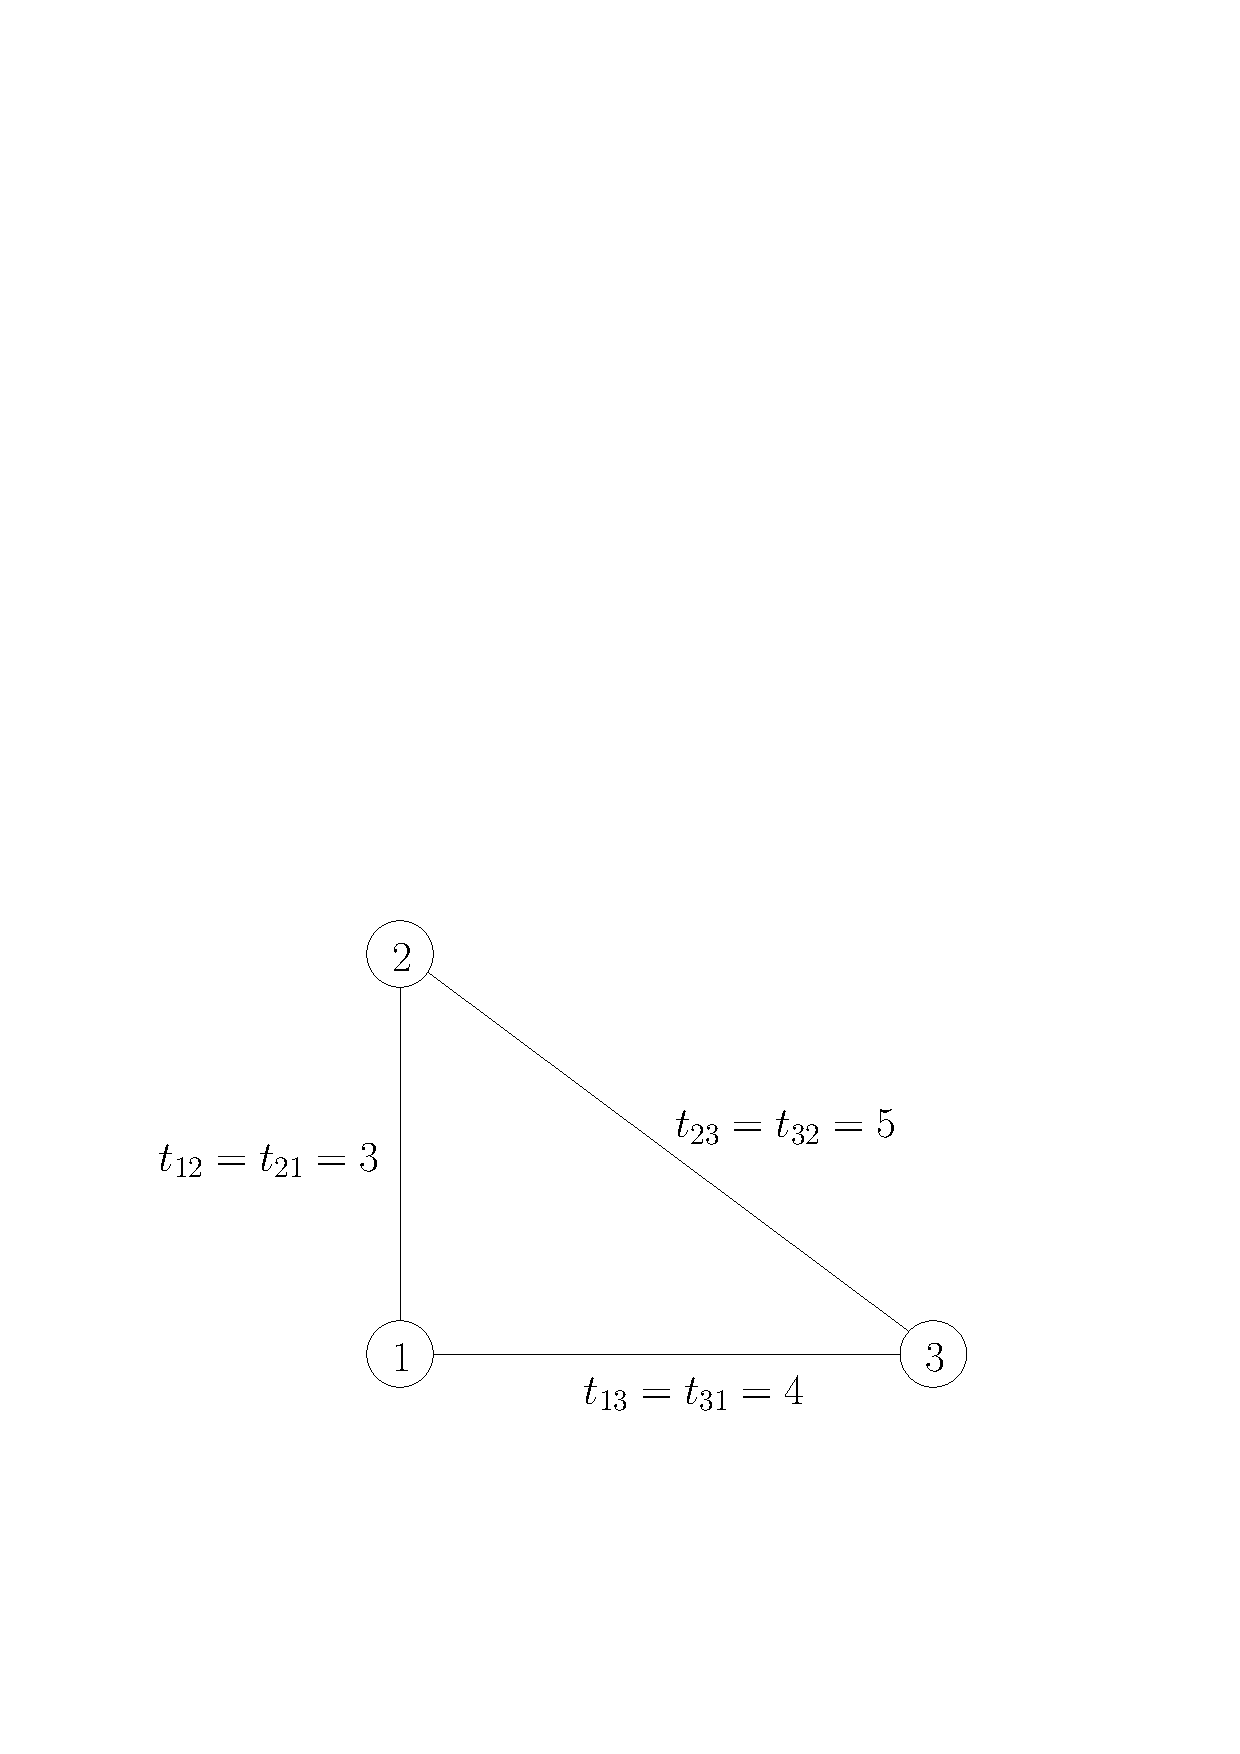
\includegraphics[width=0.4\columnwidth]{3node01}
\caption{A three node example network. The distances between the nodes 
(in kilometers) are equal to the direct ride times $t_{ij}$.}
\label{3node01}
\end{center}
\end{figure}

The solid lines in Figure \ref{convergence01} show the
arrival rates $T_s$ of vehicles at different states $s \in \mathcal{S}$ after each step of Algorithm \ref{compalg}. 
The black dashed line shows on a logarithmic scale the convergence of the norm $\|T^k - T^{k-1}\|$ 
of the difference between two successive arrival rate vectors $T^k$ and $T^{k-1}$.
The grey dashed line shows the corresponding convergence of the demand vector $Q^{\rm DRT}$.
After 28 iterations, the norm $\|T^k - T^{k-1}\|$ was less than $0.001$. 
The equilibration was continued until the norm was less than $0.00001$.

\begin{figure}[ht]
\begin{center}
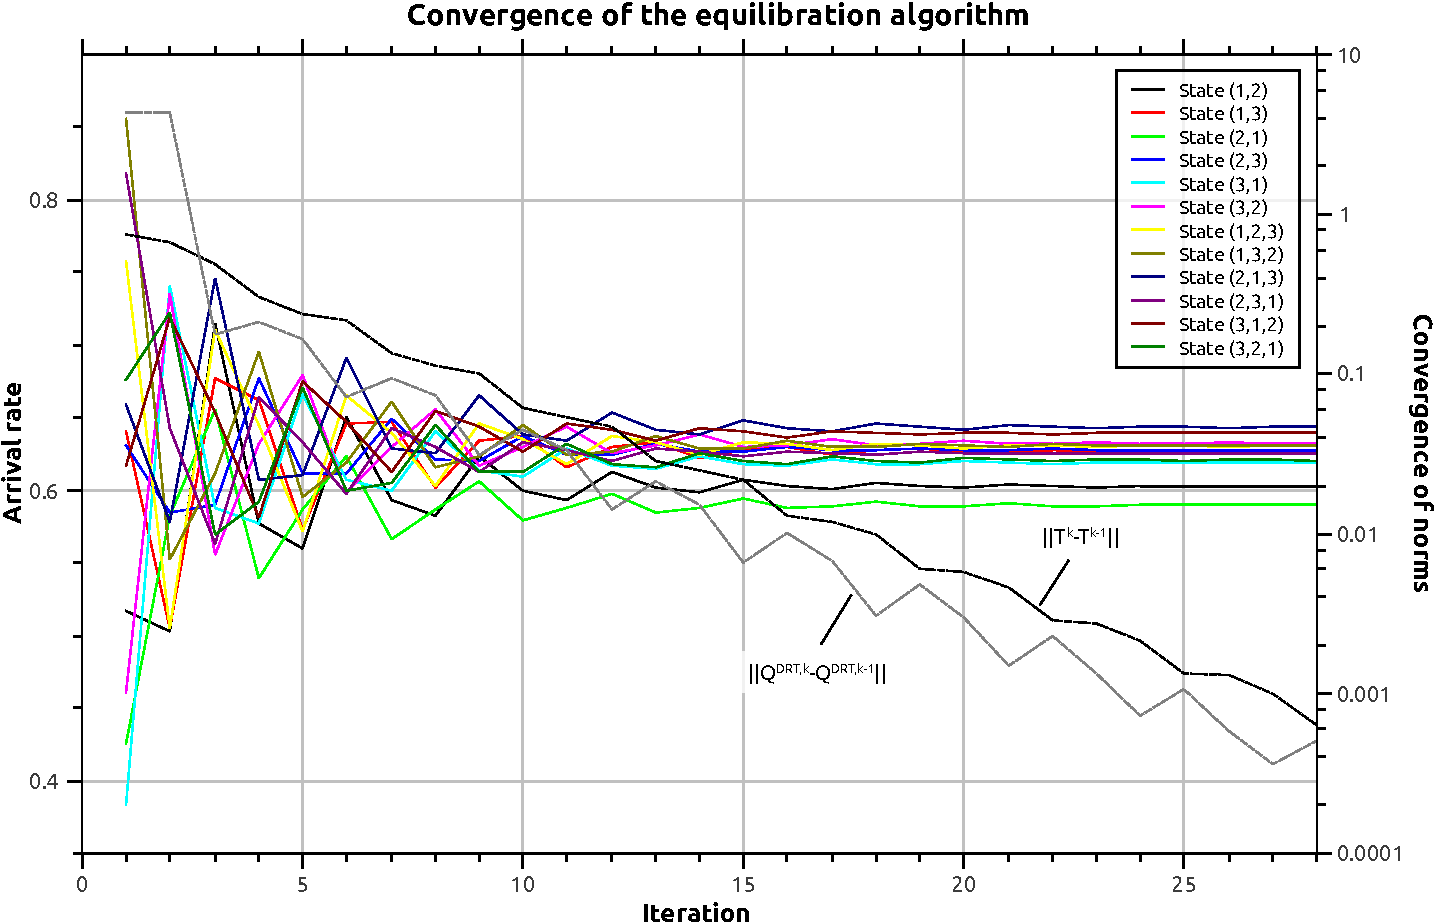
\includegraphics[width=0.9\columnwidth]{convergence01}
{\tiny
\begin{tabular}{|c|cccccccccccc|}
\multicolumn{13}{c}{} \\
\hline
\multicolumn{13}{|c|}{Arrival rates at states in the network equilibrium $T^*$} \\
\hline
State $s$ & (1,2) & (1,3) & (2,1) & (2,3) & (3,1) & (3,2) & (1,2,3) & (1,3,2) & (2,1,3) & (2,3,1) & (3,1,2) & (3,2,1) \\
\hline
Arrival rate $T_s$ & 0.603 & 0.627 & 0.590 & 0.628 & 0.619 & 0.632 & 0.631 & 0.631 & 0.644 & 0.626 & 0.639 & 0.621 \\
\hline
\end{tabular}
}
\caption{Convergence of Algorithm \ref{compalg} in the three node example. The solid lines in show the
arrival rates $T_s$ of vehicles at different states $s \in \mathcal{S}$ after each step of the algorithm. 
The black and grey dashed lines show on a logarithmic scale 
the convergence of the arrival rate vector $T$ and the demand vector $Q^{\rm DRT}$, respectively.
After 28 iterations, the norm $\|T^k - T^{k-1}\|$ was less than $0.001$. The equilibration was continued 
until the norm was less than $0.00001$. The network equilibrium is defined by the
arrival rates at different states shown in the table below the figure.}
\label{convergence01}
\end{center}
\end{figure}

By looking at the solid lines, we see the oscillatory nature of the arrival rates: When the
arrival rate of vehicles in a specific state $s$ increases during the equilibration, the number 
of customers available for a single vehicle in that state decreases. 
This causes the drivers to choose other states instead of $s$.
When the arrival rate at state $s$ decreases, it becomes more profitable for individual vehicles
and results in drivers choosing state $s$ more often. In the network equilibrium, the arrival rate is highest
at state $(2,1,3)$ and lowest at state $(2,1)$.

Referring to the dashed lines, which are roughly straight lines on a logarithmic scale, 
we see that the norms of the arrival rate and demand vectors converge exponentially
with respect to the number of iterations. Decreasing the difference $\|T^k -T^{k-1}\|$ by a factor of $F \in \mathbb{R}$
requires $G \in \mathbb{N}$ iterations. That is, $\|T^k -T^{k-1}\| = \frac{1}{F^K} \|T^{k-GK} -T^{k-1-GK}\|$
for $K \in \mathbb{N}$.
By looking at the slope of the dark dashed line, we see that the 
difference $\|T^k -T^{k-1}\|$ decreases 
by a factor of $10$ in approximately $10$ iterations, that is, $\|T^k -T^{k-1}\| = \frac {1}{10^K} \|T^{k-10K} -T^{k-1-10K}\|$
for $K \in \mathbb{N}$.




\subsection{Monopoly}
In a demand-responsive transport monopoly, a single transport operator controls the transition probabilities of vehicles
between states, in contrast to the competitive market in which the routing decisions are made by individual drivers.
In this case, the matrix $P$ containing the transition probabilities $P_{s,s'}$ is referred to as a \emph{routing strategy}.
By Equation \eqref{saapumisnopeus},
each routing strategy produces an arrival rate vector $T$ (the dominant eigenvector of $P$) that contains the arrival rates $T_s$ of
vehicles at states.

\subsubsection{Optimal routing strategies}
Let us consider three different objective functions \eqref{monopprofitrate}, \eqref{monopsurplus} and \eqref{monopwelfare}.

In an unregulated demand-responsive service operated by a single transport operator, 
the goal is to find a routing strategy $P$ that maximizes the profit rate
\begin{align}
\label{monopprofitrate}
U = \sum_{r \in \mathcal{R}}  Q_r^{\rm DRT} p_r - \sum_{s \in \mathcal{S}} T_s c_{s},
\end{align}
where $\sum_{r \in \mathcal{R}}  Q_r^{\rm DRT} p_r$ is \emph{total revenue rate} 
and $\sum_{s \in \mathcal{S}} T_s c_{s}$ is
the corresponding \emph{total cost rate}. 

Regulating the service in real-time, as described in \ref{cmonop_ecotran}, could improve the service
from the social point of view. In order to be able to study social welfare, we first define the \emph{customer surplus}
as the difference between the subjective price of the virtual mode and 
the subjective price of DRT by
\begin{align}
\label{monopsurplus}
V = \sum_{(i,j) \in I \times I} \sum_{r \in \mathcal{R}_{ij}} Q^{DRT}_r  (\bar{g}_{ij}-g_r),
\end{align}
where $Q^{DRT}_{ij}$ is the total demand for DRT trips from $i$ to $j$, $\mathcal{R}_{ij}$
is the set of DRT trips from $i$ to $j$, $g_r$ is the subjective price
of trip $r$ and $\bar{g}_{ij}$ is the subjective price of the virtual mode from $i$ to $j$.

Social welfare is defined as the sum of profit rate and surplus, that is, 
\begin{align}
\label{monopwelfare}
 W=U+V.
\end{align}

\subsubsection{Algorithm}
The idea for finding an optimal routing strategy is as follows.
First, the routing strategy $P$ is initialized and the objective function 
(for example, profit rate) is evaluated. Second, a routing strategy candidate $P'$ 
is produced by randomly perturbing $P$ and the objective function is evaluated again. 
If the value of the objective function is increased, $P'$ becomes the new routing strategy, that is, $P \leftarrow P'$. 
The second step is repeated until convergence.
The outline of the procedure is presented in Algorithm \ref{monopalg}.

\begin{algorithm}[H]
\begin{algorithmic}
\STATE \emph{Input}: Set $I$ of nodes, direct ride time $t_{ij}$, cost $c_{ij}$, demand $Q_{ij}$,
ticket price $p_{r}$, cost of virtual mode $\bar{g}_{ij}$ 
for all pairs $i,j \in I$ of nodes, number of vehicles $N$, 
customers' monetary value for unit time $\beta$
and the uncertainty parameter $\theta$.
\STATE \emph{Output}: Optimal routing strategy $P$ and the corresponding arrival rates $T_s$ of 
vehicles at states $s \in \mathcal{S}$.
\STATE Initialize the routing strategy $P$; \hfill (Transition probabilities between states) 
\REPEAT
\STATE \textbf{Arrival rates:} Solve $T_s$ for all $s \in \mathcal{S}$ by Equation \eqref{saapumisnopeus};
\STATE \textbf{Customer demand:} Calculate $E[Q_{r}^{\rm DRT}]$ for all 
$r \in \mathcal{R}$ given by Equation \eqref{drtkysynta};
\STATE Evaluate the objective function;
\IF{the value of the objective function is improved}
\STATE $P^* \leftarrow P$; \hfill (Store the current solution)
\ENDIF
\STATE Set $P \leftarrow P^* * \epsilon$ and normalize $P$, 
where $\epsilon$ is a random matrix; 
\UNTIL{convergence}
\end{algorithmic}
\caption{Equilibration of DRT.}
\label{monopalg}
\end{algorithm}

\subsubsection{A three-node example}
The three-node example described in \ref{compexample} was repeated with the maximum profit routing strategy and 
the results were compared. Table \ref{verkkovertailu} shows the total profit rate, demand and social welfare for 
the competitive market equilibrium and the profit-maximizing strategy.

\begin{table}[ht]
\begin{center}
{\footnotesize
\begin{tabular}{|c|p{2.4cm}p{2.4cm}p{2.4cm}|}
\hline
Market mechanism & Profit rate (EUR / minute) & Demand (Customers / minute) & Social welfare (EUR / minute)\\
\hline
Competitive equilibrium & 3.7 & 12.0 & 23.5 \\
Maximum profit & 5.8 & 15.6 & 35.6 \\
\hline 
\end{tabular}
\caption{Total profit rate, demand and social welfare for the competitive market equilibrium and maximum profit routing strategy.}
\label{verkkovertailu}
}
\end{center}
\end{table}

The results suggest that centralized routing strategies can be used to improve the efficiency of demand responsive transport:
By maximizing profit by means of a centralized strategy, the total profit rate, demand and social welfare are increased from
the competitive equilibrium. The difference between the mechanisms is explained by the fact that in the competitive market, 
the routing decisions are based on the drivers' incomplete market information whereas in the case of a single transport operator,
the routes are generated by using information on the state of the entire network.



\subsection{Long-run market equilibria}
\label{longrun}
In an unregulated demand-responsive transport service operated by a single operator, 
we expect that the number of vehicles and ticket price are chosen in a way that
the total profit rate is maximized in the long run.
In a competitive demand responsive market with no entry limits, 
we expect that the number of vehicles increases as long as the profit
rate of vehicles is positive. 
Regulating the number of vehicles and ticket price could improve the service
from the customers' point of view as well as from the perspective of transport operators.
In the following, we study different characteristics of demand-responsive transport
as a function of the number of vehicles $N$ and average price per kilometer $p$.
We identify the following \emph{long-run market equilibria}, defined by combinations of $N$ and $p$.

\subsubsection{Free entry equilibrium}
In the absence of entry limits in a competitive market, new vehicles arrive as long as 
the total profit rate $U(N,p)$ of vehicles is positive\footnote{We assume that the profits are 
divided equally among vehicles on average.}. 
%At some point, we expect that entry is no longer profitable. 
Thus, the feasible set for the free entry equilibrium is given by
\begin{align}
\mathcal{F} = \{(N,p) \ | \ U(N,p) \geq 0 \}.
\end{align}
In the free entry market, we assume that the drivers may agree to modify the ticket price of the service.
Thus, when the number of vehicles increases and the total profit rate approaches zero with a given 
price, the price is modified in order to keep the service profitable for the drivers.
These type of modifications result in ticket prices that attract additional vehicles to the market.
Thus, we define the free entry equilibrium by means of the condition
\begin{align}
\label{freeentry}
(N^{\rm f},p^{\rm f}) \in \{ (N,p) \in \mathcal{F} \ | \ N \geq N' \ \mbox{ for all } (N',p) \in \mathcal{F} \}.
\end{align}
That is, both the number of vehicles and price per kilometer are chosen in a way that the 
number of vehicles is maximized.

\subsubsection{Maximum profit rate}
Maximizing the \emph{total profit rate} of vehicles results in the equilibrium
\begin{align}
\label{totalprofit}
(N^{\rm tot},p^{\rm tot}) = \arg \max_{(N,p) \in \mathcal{F}} U(N,p). 
\end{align}
From the perspective of individual drivers, the optimal combination of the
number of vehicles and price is such that the \emph{profit rate per vehicle}
is maximized, that is 
\begin{align}
\label{pervehicle}
(N^{\rm 1},p^{\rm 1}) = \arg \max_{(N,p) \in \mathcal{F}} \frac{U(N,p)}{N}. 
\end{align}
 
\subsubsection{Social welfare}
Public authorities might consider regulating the DRT service in a way that it would
improve the service provided to customers as much as possible, compared
to existing transport services. The customer surplus $V$ is defined in Equation \eqref{monopsurplus}.
Similarly as in the free entry equilibrium, we require that the total profit rate of
vehicles is positive. Thus, the customer surplus equilibrium is defined by 
\begin{align}
\label{surplus}
(N^{\rm V},p^{\rm V}) = \arg \max_{(N,p) \in \mathcal{F}} V(N,p). 
\end{align}
In this case, the number of vehicles $N$ and price $p$ are regulated in a way that the 
customer surplus is maximized.

In the social welfare equilibrium, $N$ and $p$ are chosen such that the sum of profit and surplus is maximized, that is, 
\begin{align}
\label{welfare}
(N^{\rm W},p^{\rm W}) = \arg \max_{(N,p) \in \mathcal{F}} U(N,p) + V(N,p). 
\end{align}


\subsubsection{Long-run example}
The long-run market equilibria described above was determined for the three node example case introduced
in Section \ref{networkequilibrium}. The network equilibrium was calculated for different numbers
of vehicles $N$ and prices per kilometer $p$ by means of Algorithm \ref{compalg}.
For each combination of $N$ and $p$, the total profit rate, profit 
rate per vehicle and customer surplus were calculated. The results are shown in Figure \ref{a-equilibria01}.

\begin{figure}[ht]
\begin{center}
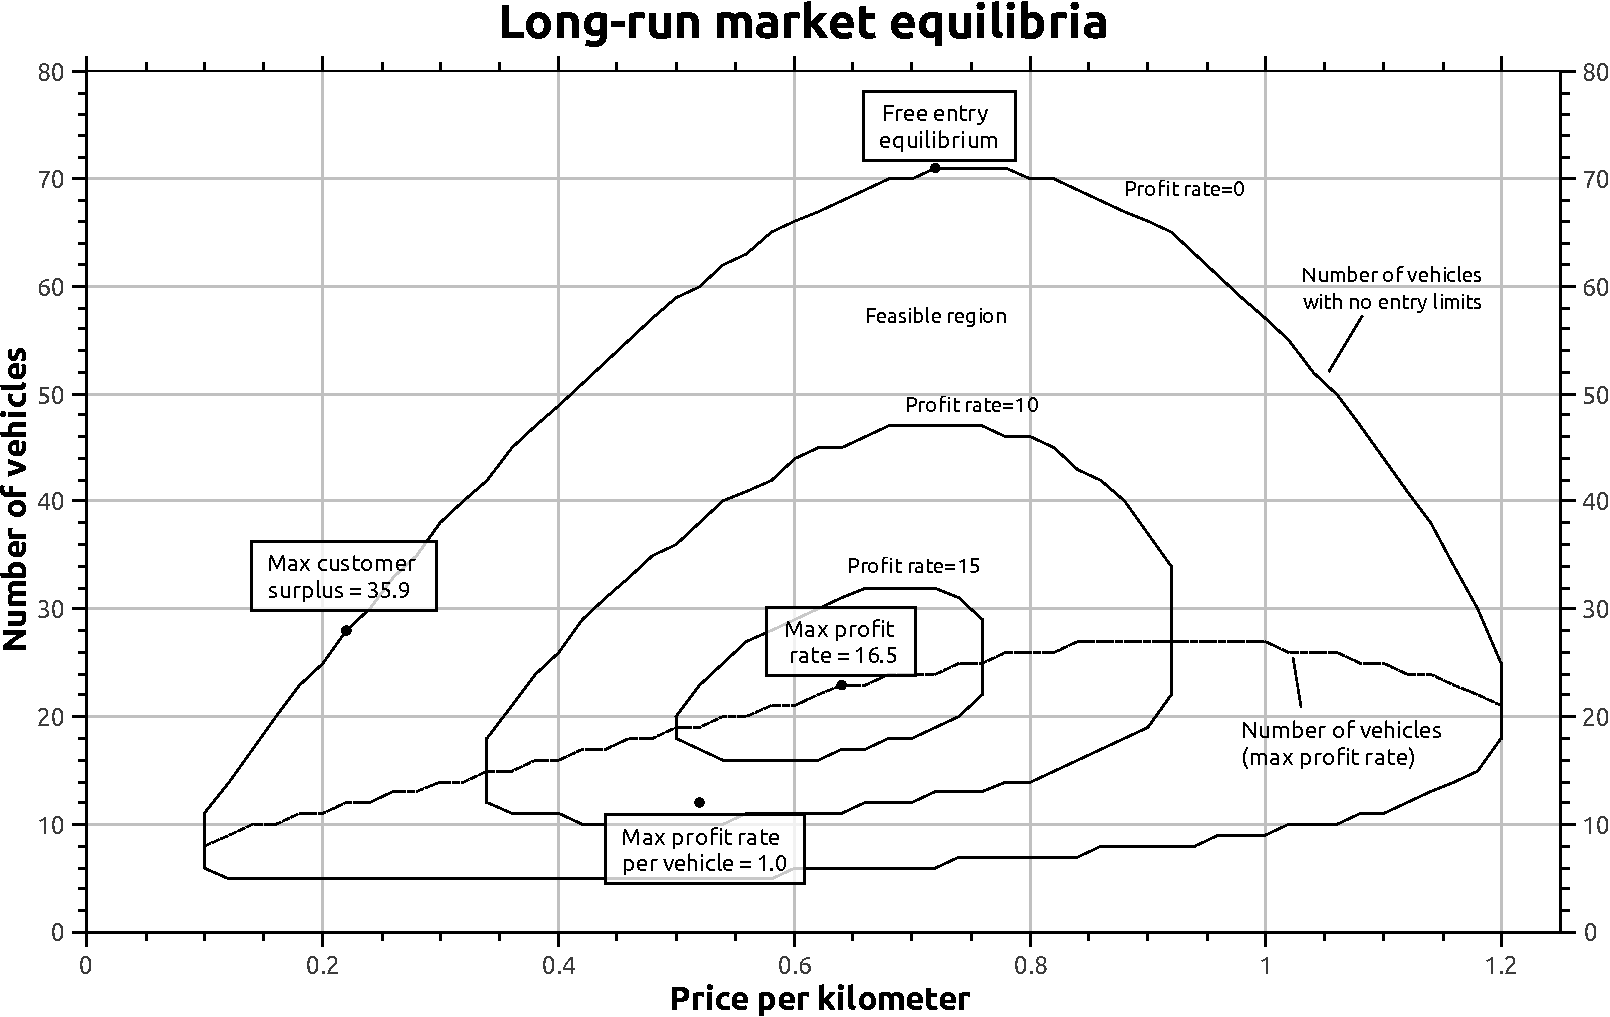
\includegraphics[width=0.9\columnwidth]{a-equilibria01}
\\
{\scriptsize
\begin{tabular}{|p{2.0cm}|p{1.0cm}|p{1.0cm}|p{1.5cm}|p{1.4cm}|p{1.2cm}|p{0.75cm}|p{0.9cm}|}
\multicolumn{8}{c}{} \\
\hline
Equilibrium & Number of vehicles & price per kilometer & Demand for DRT (customers/min) & 
Tot. profit rate / per vehicle (EUR/min) & Surplus (EUR/min) & Travel time ratio & Average occupancy \\
\hline
Max. customer surplus & 28 & 0.22 & 16.1 & 0.13 / 0.005 & 35.9 & 1.24 & 2.4 \\
\hline
Maximum total profit rate & 23 & 0.64 & 10.8 & 16.5 / 0.7 & 3.9 & 1.28 & 1.9 \\
\hline
Maximum profit rate per vehicle & 12 & 0.52 & 8.4 & 12.6 / 1.0 & 0.2 & 1.50 & 3.0 \\
\hline
Free entry equilibrium & 71 & 0.72 & 12.4 & 0.1 / 0.001 & 8.7 & 1.11 & 0.7 \\
\hline
\end{tabular}
}
\caption{Long-run market equilibria for the three node example. The first column shows the
four studied equilibrium points. The second and third columns show the 
number of vehicles and price per kilometer with which the equilibrium is achieved.
The remainder of the columns show the total demand for DRT, total profit rate and profit rate
per vehicle, customer surplus, the average ratio of travel time to direct travel time
and the average number of customers in a single vehicle.}
\label{a-equilibria01}
\end{center}
\end{figure}

The solid curves represent contour lines in which the total profit rate $U(N,p)$ of vehicles is equal ($=0,10,20$).
In particular, the outermost contour line corresponding to $U(N,p)=0$ encloses the 
\emph{feasible region}, that is, the area in which the service is profitable for drivers.
The dashed curve shows the number of vehicles for different prices for which
the total profit rate is maximized. The points represent the long-run market equilibria
defined in the previous section.

The table in Figure \ref{a-equilibria01} shows the demand for DRT, total profit rate, profit rate per vehicle, 
customer surplus, the average ratio of travel time to direct travel time
and the average number of customers in a single vehicle in the four equilibrium points.

By looking at the figure, we note that there is a significant difference between the
equilibria. In the free entry equilibrium, the number of vehicles is significantly
higher than in the other points. The average travel time ratio 
and the average occupancy are extremely low. This indicates that with no regulation, the
DRT service would approach a taxi-type service, in which all customers are 
transported privately and all trips are direct trips.

The difference in price between the free entry equilibrium and
the point in which the total profit rate is maximized is small. 
In addition, the number of served customers (demand for DRT)
is only slightly smaller in the maximum profit rate case compared to the free entry case.
However, maximizing the profit rate of vehicles would decrease the 
customer surplus and decrease the average level of service,
as can be seen by looking at the average travel time ratio and average occupancy.

The profit rate per vehicle is maximized with an extremely small number of vehicles.
In this case, only a small number of customers could be served and the level of service
would be poor.

The customer surplus is maximized by using a significantly
lower ticket price than would be optimal from the perspective of drivers. This is mainly due to the 
fact that the low price results in a high demand for DRT. Moreover, we note that the customer surplus
equilibrium is achieved by using price regulation exclusively. That is, the results suggest that 
the optimal solution from the customers' point of view would be to regulate price and allow free 
entry.





\section{Simulation model [\ref{cmonop_ecotran}]}
\label{simulationmodel}
Publications \cp{csimutools} and \cp{cmonop_ecotran} describe a microsimulation approach to 
study and compare different market mechanisms and regulation policies for
an instant-response demand-responsive transport service. An advantage of microsimulation is that 
it enables the comparison of different market mechanisms and regulation policies on a detailed level:
For example, the model can be used to study scenarios involving multiple competing vehicle operators,
each of which seeks to maximize its total profit (typical structure of conventional taxi-markets), as well as
scenarios involving a monopoly service operator.

The simulation model is governed by the following preliminary assumptions.
\begin{enumerate}
\item
There are $K$ vehicles available for transporting customers requesting service within a certain operating zone $A$. For each pair of points $a$ and $b$ in $A$, the distance $d(a,b)$ and direct ride time $t(a,b)$ are known and equal for all vehicles.
\item
At each moment, each vehicle is assigned a certain set of customers and a tentative (shortest) route passing through all 
unvisited pick-up and drop-off points associated with these customers. 
\item
At any moment, a new customer may request a trip from a specific pick-up point $a$ to a specific drop-off 
point $b$.
\item
As an instant response to each customer request, one or several trip offers are presented to the customer, from which the customer
accepts at most one. If an offer is accepted, the customer is assigned to the corresponding vehicle and the route of the vehicle
is modified (see Figure \ref{dynamicexample07}).
	\item
	There is a fixed fare structure. 
	The price $R$ of a trip is assumed to be dependent on the direct trip 
	length $d(a,b)$ exclusively by means of the formula
	\begin{align}
R(a,b)=p\cdot d(a,b),
\end{align}
where $p$ is the price per kilometer in relation to direct trip length.
% The customers know the fare structure and the direct trip lengths beforehand.
\end{enumerate}






\begin{figure} %[ht]
\begin{center}
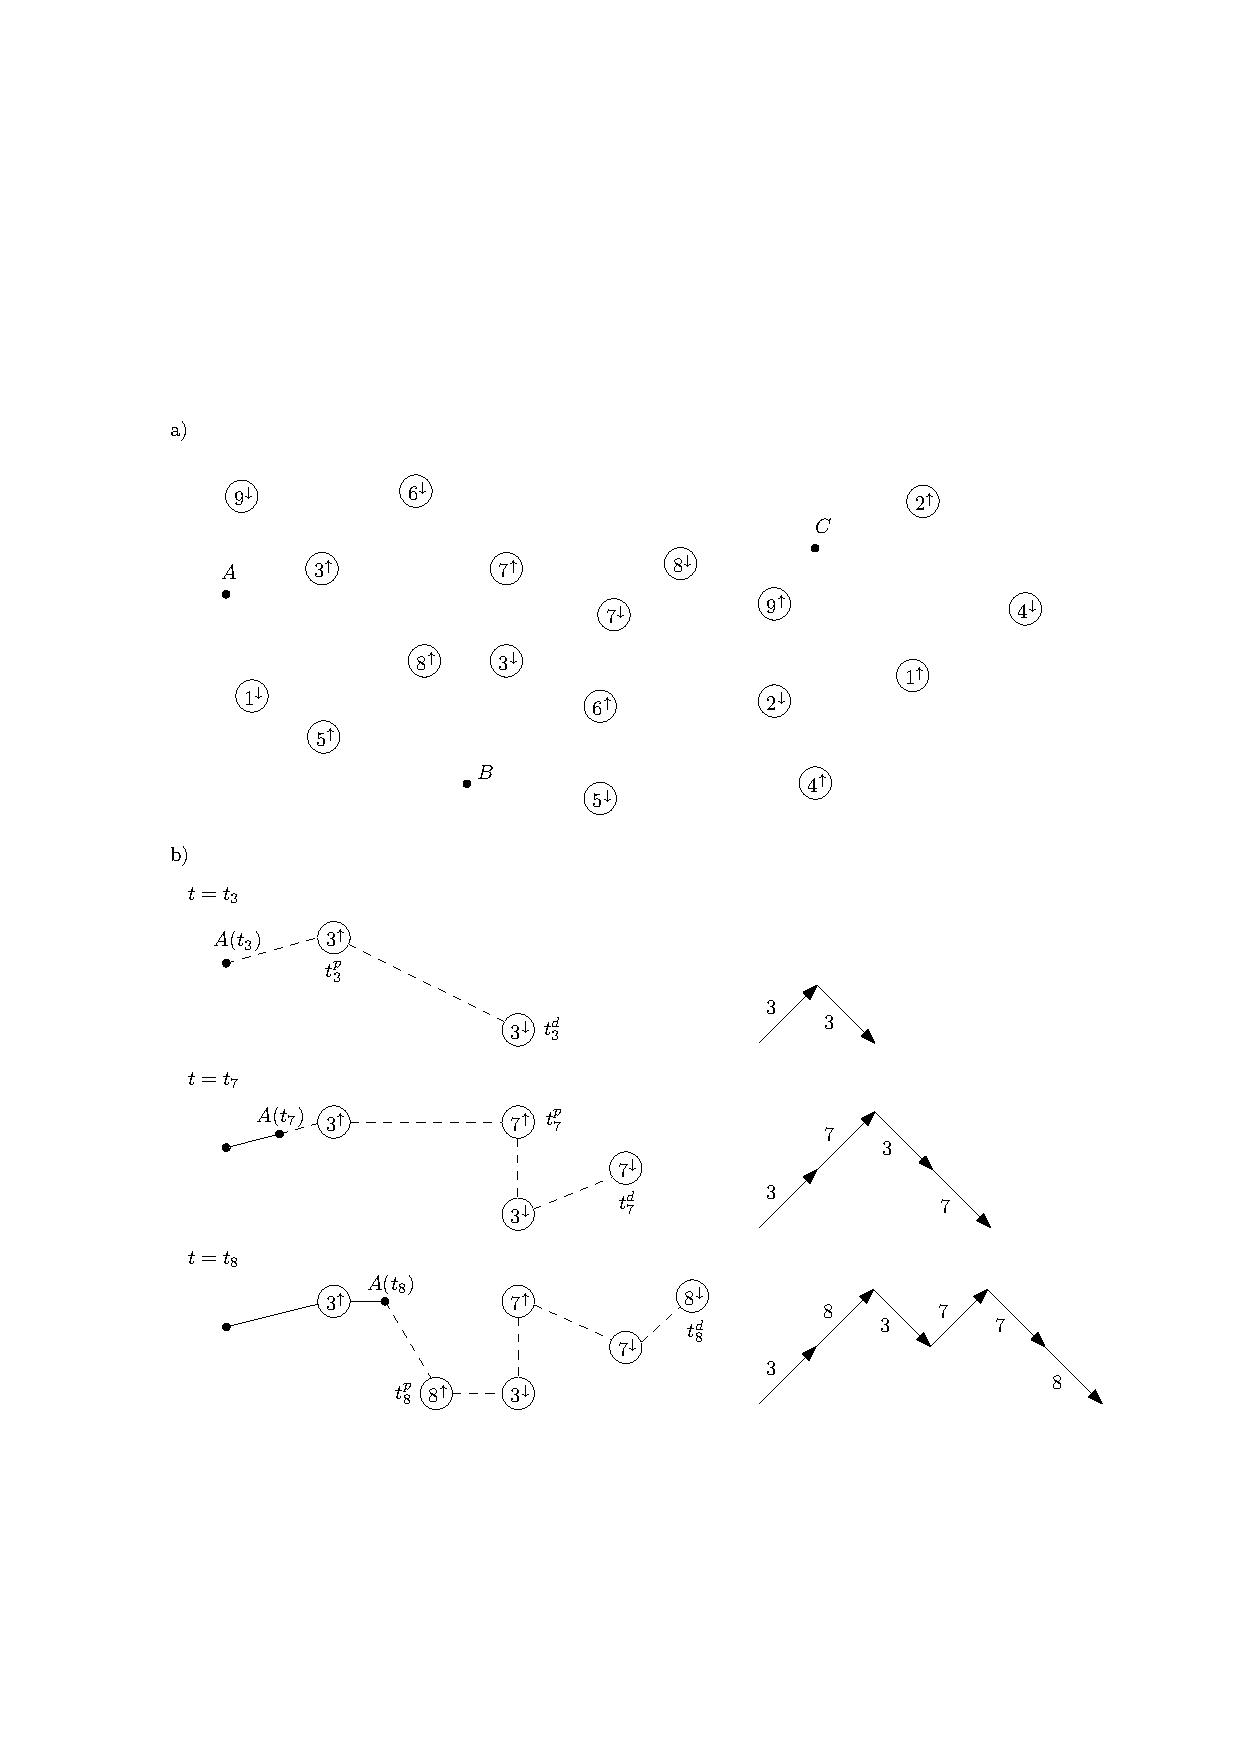
\includegraphics[width=1.0\textwidth]{dynamicexample09}
\caption{Route modifications. The top figure (a) shows the pick-up points (denoted by $\uparrow$-signs) and drop-off points ($\downarrow$-signs) of
nine customers and the initial locations of vehicles $A,B$ and $C$. Each customer $i$ requests a trip from $i^{\uparrow}$ to $i^{\downarrow}$
at time $t=t_i$, where $t_1 < t_2 < \ldots < t_9$. The bottom figure (b) shows the modifications in the route of vehicle $A$. 
At the time customer $3$ requests a trip ($t=t_3$), the vehicle is located at $A(t_3)$. A new route for the vehicle, namely ($3^{\uparrow},3^{\downarrow}$), beginning from $A(t_3)$ is calculated and the expected pick-up and drop-off times, $t_3^p$ and $t_3^d$, 
are determined by means of the new route. Customer $3$ accepts the offer and the vehicle route
is updated. Customers $7$ and $8$ are added to the vehicle route in a similar fashion.
The figures on the right show the routes as so-called labeled Dyck 
paths \citep{cori, eadarp},
%\footnote{The term "labeled Dyck path" was introduced in \citep{cori}. 
%The number of labeled Dyck paths involving $n$ customers is equal to $(2n)!/2^n$ .}
%\protect\footnotemark[5]
in which each pick-up $i^{\uparrow}$ precedes the corresponding drop-off $i^{\downarrow}$. 
After each step, a new path is formed due to the addition of a new customer. Clearly, the "height" of the path
shows the number of customers aboard in different parts of the route.
}
\label{dynamicexample07}
\end{center}
\end{figure}

\subsection{Demand}
The level of service is determined by \emph{travel time ratio}, which describes the ratio of travel time to direct ride time.
In other words, a travel time ratio equal to one corresponds to the best possible level of service and 
a larger travel time ratio corresponds to a lower level of service. 

Since the fare structure for trips is assumed to be fixed, 
the only question a customer faces after requesting service is whether or not to accept the best transportation offer in terms
of the level of service. 
The level of service offered to a customer traveling from $a$ to $b$ is defined by means of travel time ratio
\begin{align}
\tau=\frac{t_d-t_r}{t(a,b)},
\end{align}
where $t_d$ is the drop-off time, $t_r$ is the release time of the request and $t(a,b)$ is the direct ride time from $a$ to $b$. 

The demand model is expressed by means of a probability distribution $P(\mbox{accept} \ | \ \tau,p)$, 
which denotes the conditional probability that an arbitrary customer accepts an offer with travel time ratio $\tau$ and price $p$. 
An example of a linear acceptance probability function is illustrated in Figure \ref{acceptanceprob01}. The relation 
to alternative transportation modes is clarified in Figure \ref{acceptanceprob02}, which shows the basic idea behind the linear demand model.

\begin{figure} [ht]
\begin{center}
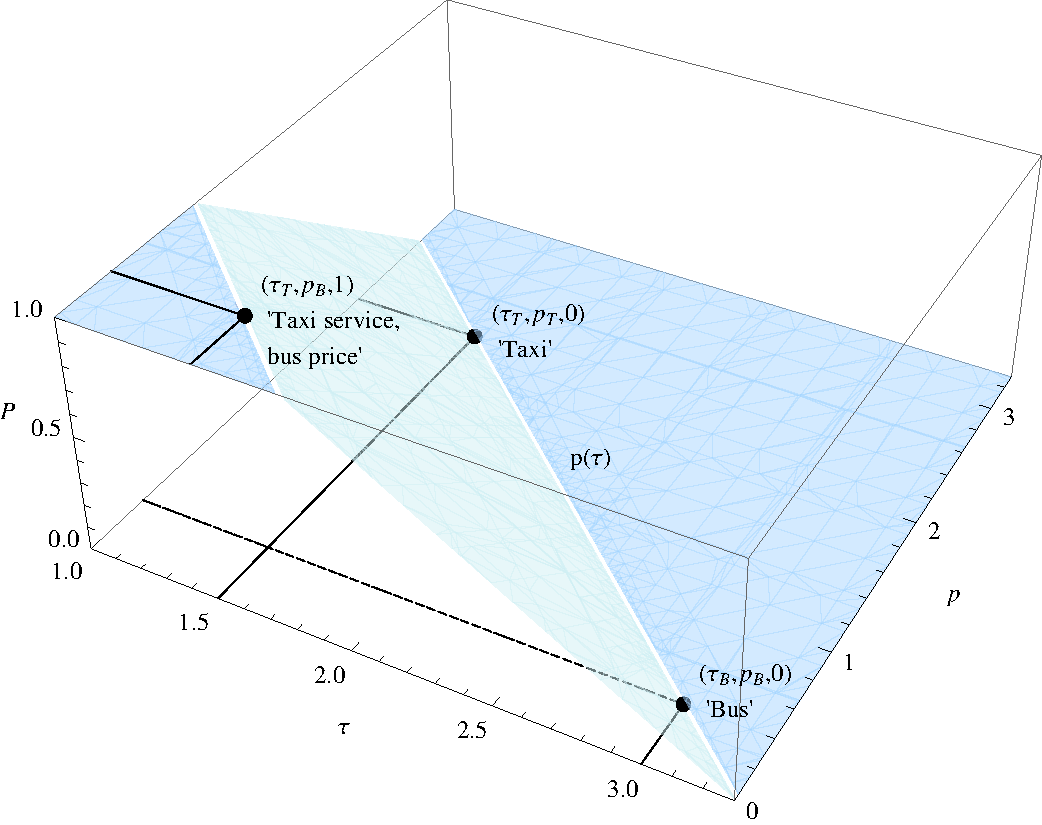
\includegraphics[width=0.9\textwidth]{acceptanceprob01}
\caption{A linear example of the acceptance probability function $P(\mbox{accept} \ | \ \tau, p)$. The linear function is
specified by means of three points representing conventional bus and taxi services and a taxi-type service for the price of a bus. 
}
\label{acceptanceprob01}
\end{center}
\end{figure}


\begin{figure} [ht]
\begin{center}
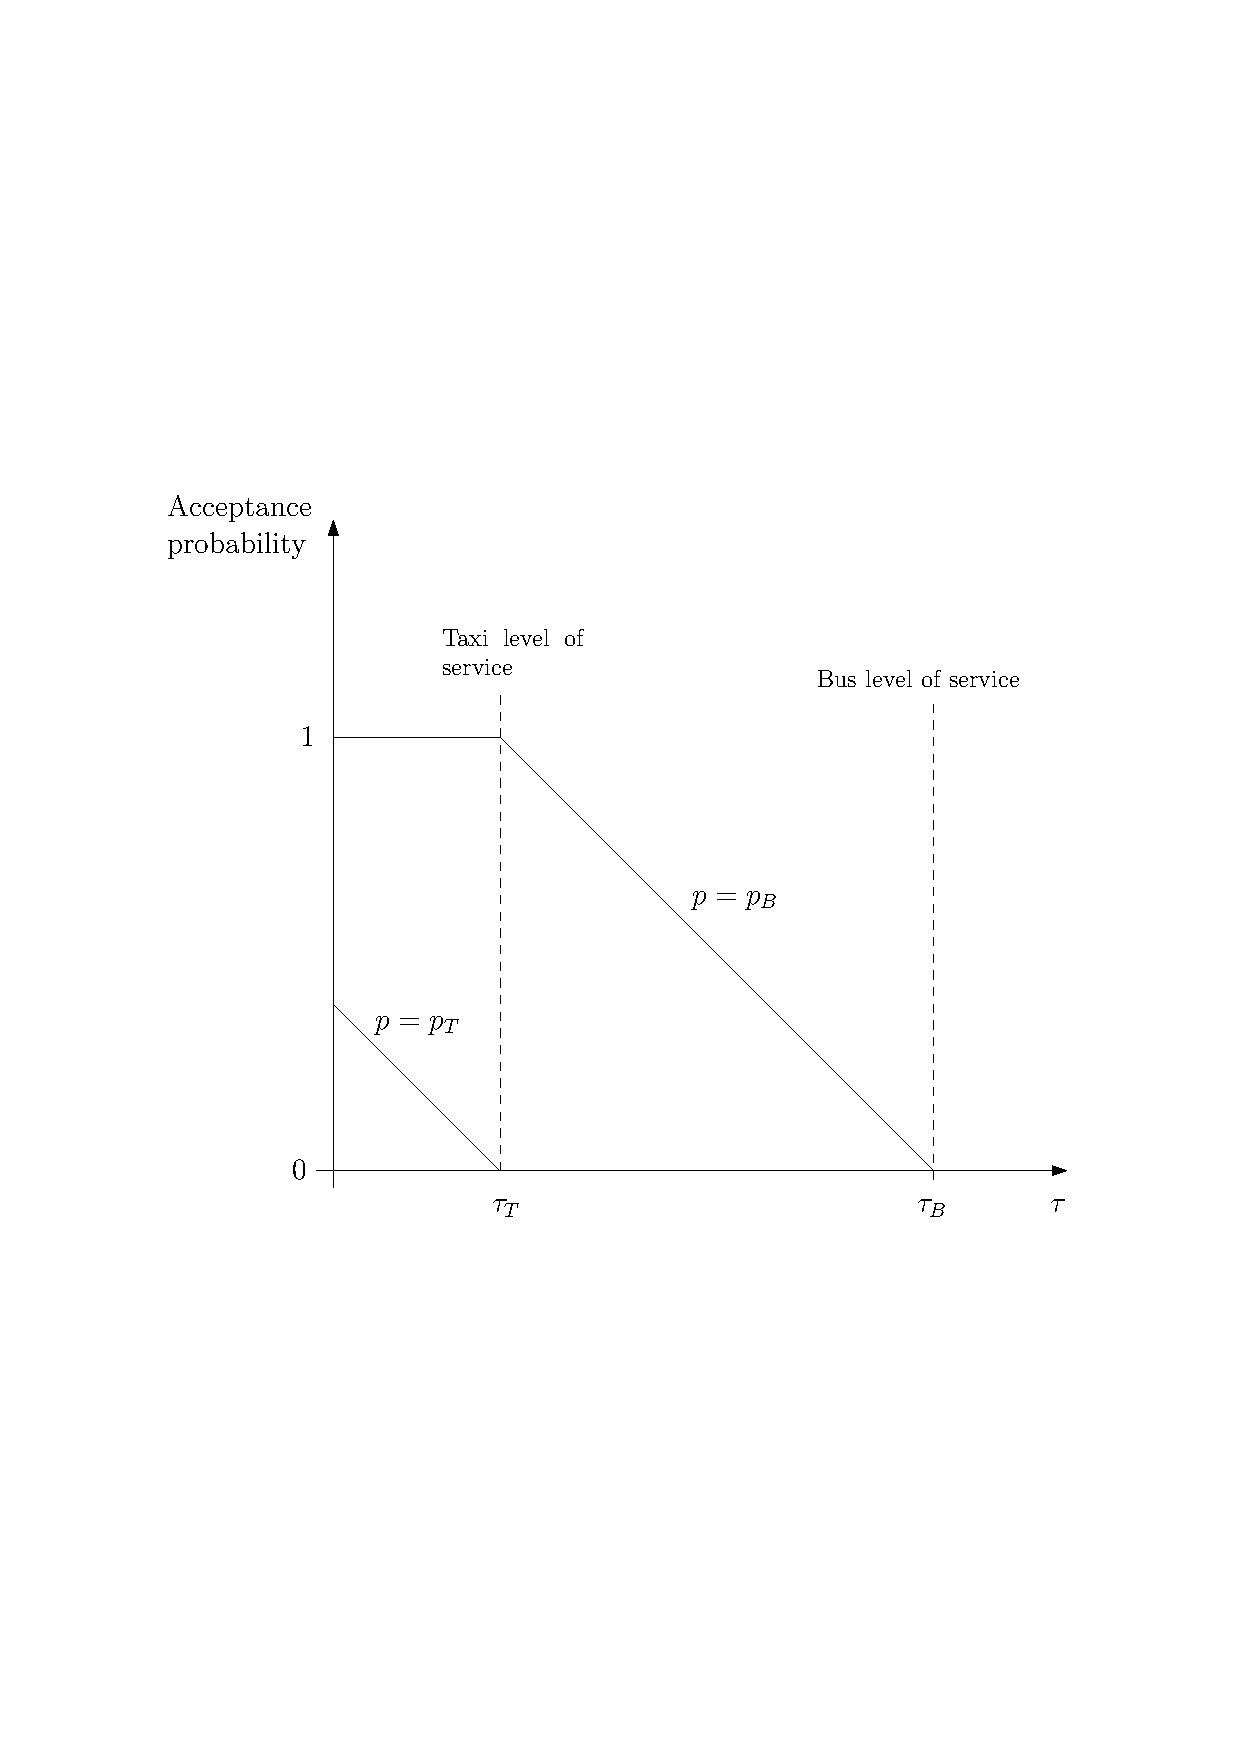
\includegraphics[width=0.6\textwidth]{acceptanceprob2}
\caption{The linear acceptance probability function related to alternative transportation modes. 
If the level of service is as good as that of a normal taxi 
($\tau = \tau_T$) and the price is equal to the price of a bus ($p=p_B$), any customer is likely to accept the demand-responsive transport service. The fraction of customers willing to accept the service decreases with the level of service. If the price and level of service are equal to the taxi ($p=p_T$ and $\tau=\tau_T$), the acceptance probability is zero.
}
\label{acceptanceprob02}
\end{center}
\end{figure}

\subsection{Supply}
\label{dailydecisions}
Let us present the following mechanisms for generating trip offers at the time a customer request is released: 

\textbf{Monopoly:} In order to maximize total profit, the monopolist formulates a single offer in a way that the additional cost of 
providing service is as small as possible and the probability that the customer accepts the offer is as high as possible. In other words, 
the monopolist chooses for each trip $(a,b)$ a vehicle in a way that the expected profit
\begin{align}
\label{dailymonopoly}
\E{\pi}=P(\mbox{accept} \ | \ \tau, p) \cdot \Big( p -\E{\Delta C} \Big)
\end{align}
is maximized, where $P(\mbox{accept} \ | \ \tau, p)$ denotes the acceptance probability with level of service $\tau$, price $p$ and 
$\E{\Delta C}$ denotes the expected increase in the cost of the vehicle route caused by the new potential customer.

\textbf{Competitive market:}
For each vehicle, a new route serving the new potential customer and the previously assigned customers
is computed. The best vehicle from the customer's point of view is the one that
provides the smallest travel time ratio $\tau^*$. The customer chooses the trip offered by this vehicle with probability
$P(\mbox{accept} \ | \ \tau^*, p)$.


\subsection{Simulation experiments}
\ref{csimutools} describes a simulation model, where trip requests occur within a bounded region in a plane. Each trip request is defined as a triple, $(t_i, a_i,b_i)$, where $t_i$ denotes the release time of request $i$, $a_i$ and $b_i$ denote the origin and the destination of the trip, respectively. There are $K$ vehicles each with capacity of $c$ customers. 
When a trip request arrives, it is immediately assigned to a single vehicle. The chosen vehicle then carries the customer from the origin to the destination. With $c>1$, several customers can share a vehicle, which allows the system to combine trips and decrease the effort per customer.
A constant velocity $v$ and a constant minimum stop time of $t_{\mbox{st}}$ is assumed for each vehicle. The minimum stop time is assumed to include the time needed for deceleration and acceleration. 

\ref{cmonop_ecotran} extends this model by the following modification:
Upon arrival of a trip request, it is assigned to a single vehicle, assuming that the customer accepts the 
best trip offered by the studied market mechanism, that is, with probability $P(\mbox{accept} \ | \ \tau, p)$.
If the customer does not accept the best offer, no vehicle routes are modified.

\subsubsection{Long-run market equilibria}
Similarly as in Section \ref{longrun}, the simulator is used to find the optimal number of 
vehicles $K$ and price per kilometer $p$ in two mechanisms: 
1) monopoly and 2) competitive market.
In both mechanisms, the objective is to maximize profit. The optimal values $K^*$ and $p^*$
are determined for each mechanism by running the simulator with different values of $K$ and $p$ and choosing the
best combination with respect to the objective, see Figure \ref{simulationkuva}. 

\begin{figure} [ht]
\begin{center}
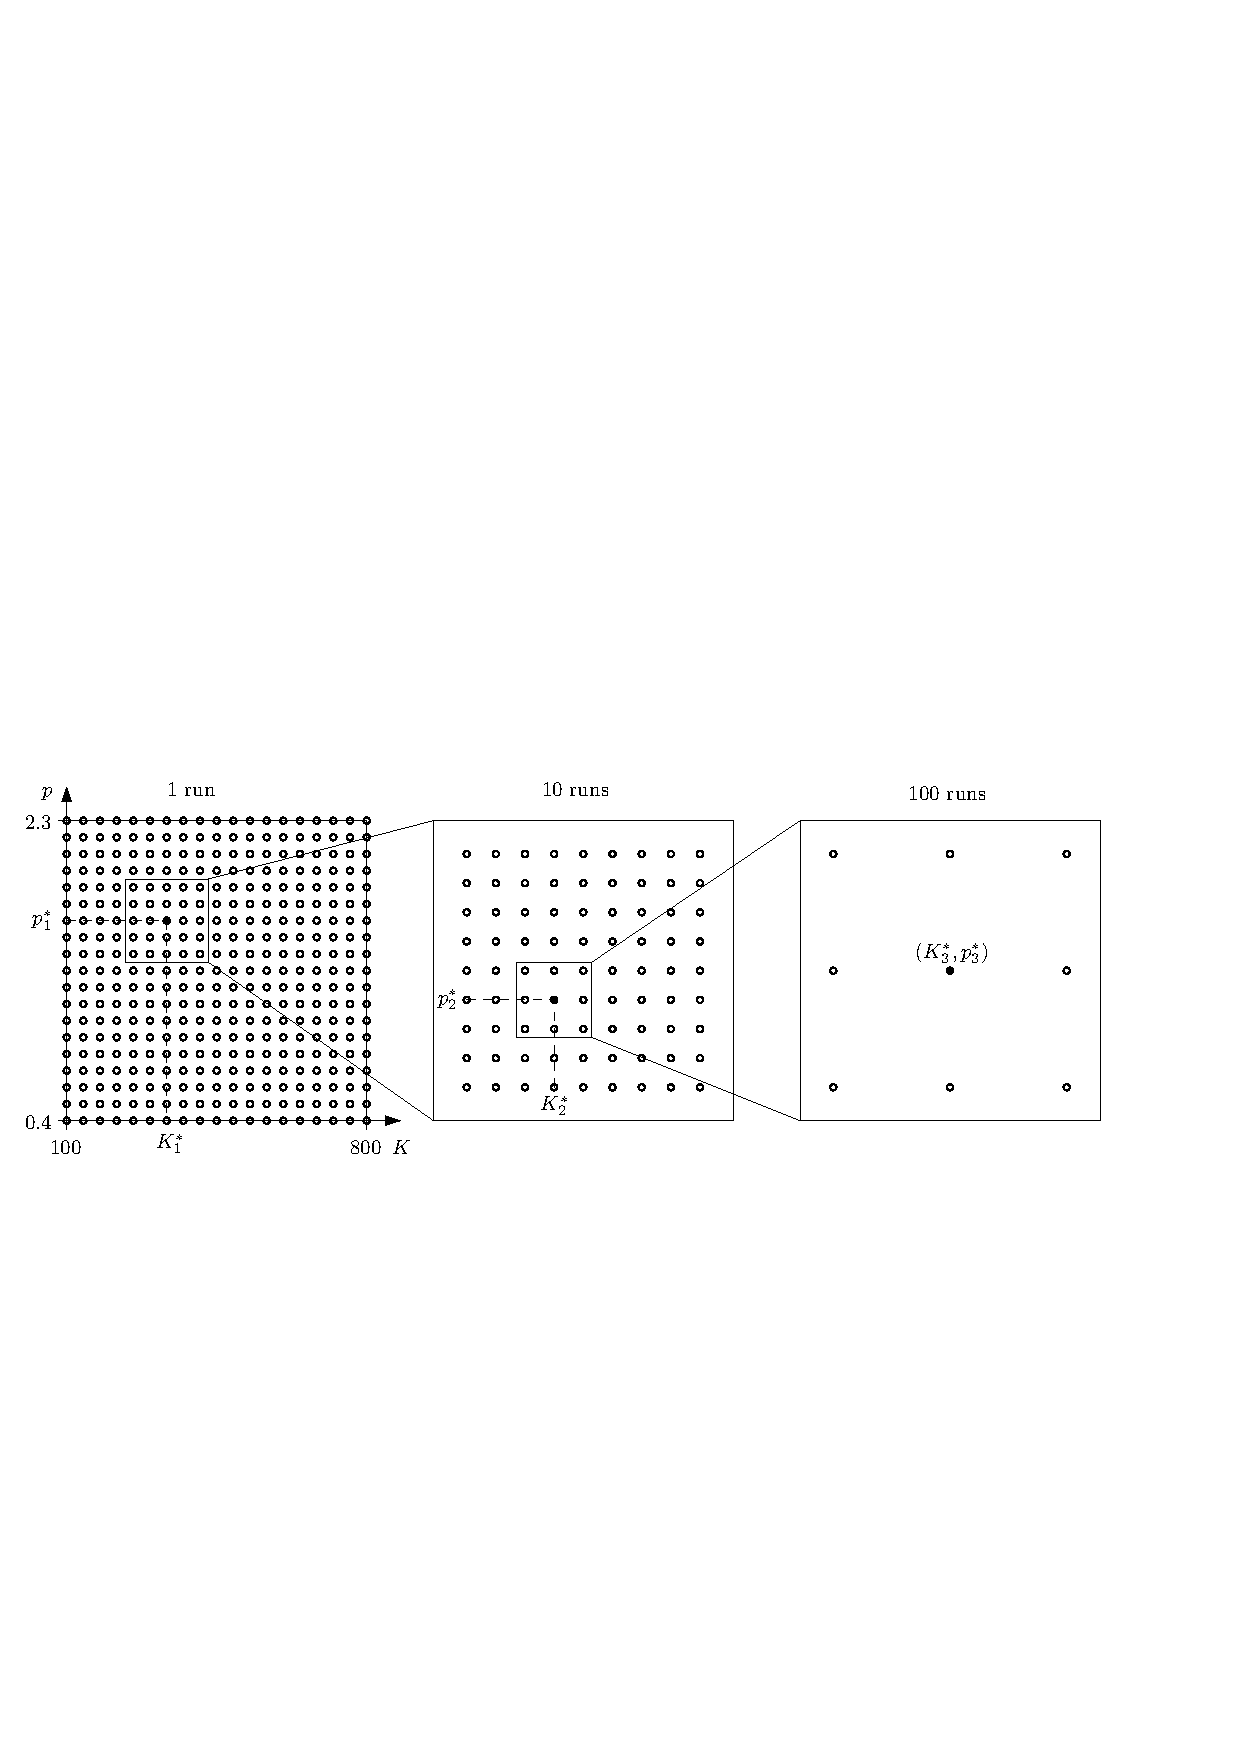
\includegraphics[width=\textwidth]{simulation02}
\caption{Determining optimal number of vehicles $K$ and price per kilometer $p$ by means of 
simulation. At first, an initial run is executed for each $(K,p) \in \{100, 110, \ldots, 800\} \times \{0.4, 0.45, \ldots, 2.3\}$.
Then, the optimum $(K^*_1,p^*_1)$ is updated by narrowing the parameter space to 81 points chosen from the neighborhood of the optimal point and 
performing 10 runs for each point, yielding $(K^*_2,p^*_2)$.
Finally, a new optimum is determined by performing 100 runs for nine points in the neighborhood of the previous optimum. 
The last step is repeated until convergence.} 
\label{simulationkuva}
\end{center}
\end{figure}

\subsubsection{Results}
Table \ref{tulokset} presents the long-run equilibria for the studied market mechanisms. The table shows the optimal price per kilometer and the optimal number of vehicles for the market mechanisms together with the corresponding daily profit, customer surplus and social welfare, that is, the sum of the profit and surplus. In addition, the number of served customers, average realized travel time ratio and relative driven distance are given. The average travel time ratio is determined by dividing the total travel time of customers by the sum of direct trip ride times. Thus, it describes the average level of service experienced by the customers. The relative driven distance is calculated by dividing the total distance driven by vehicles by the sum of direct trip lengths. Consequently, it describes how efficiently the vehicles are utilized. 

\begin{table}
\centering
{\scriptsize
\begin{tabular}{|lrrrrrrrr|}
\hline
Mechanism & Number of &	Price/ & Surplus	& Profit	& Social & Served & Travel time& Relative \\
& vehicles $K$ &  km $p$ & & & welf. & cust. & ratio & dist. \\
\hline
1) Monopoly	                & 210	& 1.65	& 417	  & 94535	& 95429 & 21213	& 1.688	& 0.613 \\
3) Competitive market 	    & 700	& 1.70	& 47040	&  985	& 48025	& 26041	& 1.268	& 1.024 \\
\hline
\end{tabular}
}
\caption{Simulation results. The first columns of the upper table show the 
optimal number of vehicles $K$ and price per kilometer $p$ for the studied mechanisms. The remaining
columns show the corresponding daily surplus, profit, social welfare, 
number of served customers, realized travel time ratio and relative driven distance.}
\label{tulokset}
\end{table}

From table \ref{tulokset}, one can observe that while the monopoly mechanism yields more profits than the competitive market, focusing only on profit will wither the total customer surplus. The distance driven by the vehicles is 39\% lower compared to
the sum of direct trip lengths, which suggests that the vehicles are utilized efficiently.

In the competitive market mechanism, the number of vehicles that are allowed to enter the market is not limited. The market attracts new vehicles as long as there are excess profits available. The profit of the competitive market would thus finally approach zero. However, the large number of vehicles could provide a relatively good level of service for customers, as can be seen from the total surplus and average travel time index. 
The travel time of customers is increased only by 27\% compared to the direct trips. Thus, the competitive market is seen to
provide a service comparable to conventional taxi.

The results presented in \ref{cmonop_ecotran} suggest that the social welfare can be further increased by 
regulating the monopoly mechanism in real time. This means that instead of expected profit, trip offers are generated by maximizing 
the sum of expected profit and customer surplus. 
%In addition, the number of vehicles and price are
%regulated in a way that the social welfare is maximized.


\chapter{Conclusions}
\label{conclusions}
This work presents mathematical models for demand-responsive transport and methods
that can be used to solve combinatorial problems related to vehicle routing and journey planning
in a transport network.

First,
we show how the demand for transportation can be satisfied by constructing routes for a fleet of vehicles,
assuming that the origins, destinations and time limits of customers' trips are known.
Then, by considering a stochastic journey planning problem in a public transport network we determine
the optimal actions of commuters, assuming that the vehicle routes are fixed during a specific time horizon.
Finally, we present methods based on microsimulation and analysis
for determining the economic equilibrium, that is, the point at which the demand meets the supply,
by assuming that commuters attempt to minimize travel time and transport operators aim to maximize profit.

The proposed models can be used to simulate the operations of public transport services ranging 
from paratransit services for the elderly and disabled to 
large-scale demand-responsive transport services. These calculations can 
provide valuable information to public authorities and planners of transportation services,
regarding, for example, regulation and investments.
In addition to public transport, potential applications of the proposed methods for solving vehicle routing and journey planning problems
include freight transportation, courier and food delivery services, military logistics and air traffic.

%This work is focused on combinatorial problems arising from the planning of demand responsive transport.
%Particularly, the single vehicle dial-a-ride problem and related problems are studied.

% In chapter \ref{irdarp}, a decentralized algorithm for
% real-time demand responsive transport is described.
% The proposed solution makes use of communication between
% customers requesting service and vehicles providing service in a way
% particularly suitable for a highly dynamic service, in which
% a vast majority of requests are formed not long before the customer
% requesting service is willing to depart. 
% An algorithm for solving the dynamic single vehicle dial-a-ride
% problem is used as a subroutine in the multiple-vehicle problem. 
% In order to achieve high-quality results, an exact algorithm for the single vehicle dial-a-ride problem
% should be incorporated. In some applications, however, this may not be feasible since such an algorihm 
% would require too much computational work. On the other hand, the use of heuristics, such as the insertion algorithm
% (see for example \cite{jaw}) may significantly degrade the performance of the service in some cases.
% 
% In chapter \ref{eadarp}, an exact optimization procedure is developed to solve the
% static and dynamic versions of the single vehicle dial-a-ride problem with time 
% windows. Using complete enumeration to solve the problem with respect
% to a generalized objective function is motivated by the dynamic nature of 
% online demand responsive transport services,
% in which looking only at the tentative route duration, as in existing algorithms for the problem,
% may decrease the possibilities of serving future customers.
% In addition, an adjustable heuristic extension to the algorithm
% is introduced, in order to be able to control the CPU times:
% If the problem size is reasonable, the proposed solution method
% produces globally optimal solutions. If the problem size is increased, 
% the algorithm adjusts itself to produce locally optimal solutions,
% closing the gap between the classical insertion heuristic and the exact solution and thus
% making the algorithm applicable to any static or dynamic dial-a-ride problem.
% 
% Chapter \ref{tspdn} focuses on the effect of walking on the performance of
% demand responsive transport. The problem of redirecting customers is modeled by means of the traveling salesman
% problem with disk neighborhoods, in which each node can be redirected
% to another location within a certain maximum walking distance from the original location. 
% By means of differential analysis, an upper bound for the decrease 
% in the length of a vehicle route is derived for the Euclidean, Manhattan and
% hyperbolic metrics. The main result is that the effect of walking is strongly dependent on the sharpness of turns in
% a vehicle route: if all customers are located along the same road, no advantage is gained by redirecting. 
% On the other hand, if the service is near door to door, the distance driven by
% the vehicle may be reduced up to 2 times the total walking distance of customers.
% 
% In chapter \ref{simutools}, an immediate request dynamic vehicle routing problem with pick-ups and deliveries is studied.
% The focus is on systems where a large number of vehicles are needed to support
% the transportation demand. As a particular feature of the system, a vehicle is assigned to
% each customer immediately upon the trip request. Simulation experiments are used to show that 
% that in this context it is typically sufficient, without any significant loss in performance, to consider
% the insertion approach for route enumeration, where the relative order
% of the earlier waypoints is always kept the same. 
% That is, it is not necessary to enumerate
% {\em all} feasible orders of waypoints per trip request and per
% vehicle, which indeed can take some time in a large system. % with high load.
% On the other hand, the viability of this type
% of transportation system is demonstrated by means of simulation experiments. In general, there is a well-known
% trade-off between the work conducted (driven kilometers)
% and the level of the service (e.g., mean waiting times).
% However, the experiments suggest that if the customers are
% willing to accept even a small average delay for their trips,
% in form of waiting time and/or a longer route, then
% the amount of work can be reduced considerably. That is, the
% transportation cost per trip can be reduced significantly.

As a final conclusion, it can be stated that there are many theoretical results
that support the technical viability of demand-responsive transport.
However, as suggested in \cite{cortes}, one of the key issues in a large scale demand 
responsive service ever becoming a reality, is the
institutional inertia against change in transit paradigms. No models exist that are
directly applicable in finding to what extent a completely new transportation system is possible in real life.
How to accurately estimate the demand for a hypothetical transportation service remains a relatively open question.
In order to be able to access such practical problems, future work calls for 
real-life pilot services, which would probably give valuable information on the 
demand for and performance of demand-responsive transport.






%% The following commands are for article dissertations, remove them if you write a monograph dissertation.

% Errata list, if you have errors in the publications.
%\errata

\bibliographystyle{plain}
\bibliography{dju,vk,eadarp,hitsdarp,hitsdarp2,kuhmo}


%% The first publication (journal article)
% Set the publication information.
% This command musts to be the first!
\addpublication{Lauri H\"ame}{An adaptive insertion algorithm for the single-vehicle dial-a-ride problem with narrow time windows}{European Journal of Operational Research}{209, p. 11–22}{February}{2011}{Elsevier B.V.}{jeadarp}
% Add the dissertation author's contribution to that publication (the order can be interchanged with \adderrata).
\addcontribution{This article was written by the author.}
% Add the errata of the publication, remove if there are none (the order can be interchanged with \addauthorscontribution).
%\adderrata{This is wrong}
% Add the publication pdf file, the filename is the parameter (must be the last).
\addpublicationpdf{articles/eadarpejor.pdf}

%% The second publication (conference article, note the optional parameter)
% Set the publication information.
\addpublication[conference]{Esa Hyyti\"a, Lauri H\"ame, Aleksi Penttinen, Reijo Sulonen}{Simulation of a Large Scale Dynamic Pickup and Delivery Problem}{SIMUTools}{Malaga, Spain}{March}{2010}{ICST}{csimutools}
% Add the dissertation author's contribution to that publication.
\addcontribution{Parts of this paper were written the author, including most of Section 3 and parts of Section 1. 
The simulations reported in Section 3 were designed and conducted by the author.}
% No errata
% Add the publication pdf file, the filename is the parameter.
\addpublicationpdf{articles/simutools-2010b.pdf}

\addpublication[conference]{Lauri H\"ame, Jani-Pekka Jokinen, Reijo Sulonen}{Modeling a competitive demand-responsive transport market}{Kuhmo Nectar Conference on Transport Economics}{Stockholm, Sweden}{June-July}{2011}{No copyright holder at this moment}{ccompejor}
\addcontribution{The author was the main author of this article, which was nominated for the best student paper award in Kuhmo Nectar 2011.
The article is under review for publication in Economics of Transportation.}
\addpublicationpdf{articles/compejor.pdf}

\addpublication[conference]{Jani-Pekka Jokinen, Lauri H\"ame, Esa Hyyti\"a, Reijo Sulonen}{Simulation Model for a Demand Responsive Transportation Monopoly}{Kuhmo Nectar Conference on Transport Economics}{Stockholm, Sweden}{June-July}{2011}{No copyright holder at this moment}{cmonop_ecotran}
\addcontribution{Parts of this paper were written the author, including major parts of Sections 2 and 3.
The market mechanisms were programmed into the simulation model and the simulations were executed by the author.
The author produced the figures in this paper and the idea of using the simulation model reported in 
"Simulation of a Large Scale Dynamic Pickup and Delivery Problem" to study market mechanims was originally suggested by the author.
This paper is also under review for publication in Economics of Transportation.
}
\addpublicationpdf{articles/monop_ecotran.pdf}

%% The third publication (another journal paper, accepted for publication, note the optional parameter)
% Set the publication information, detailed information can be empty
\addpublication[conference]{Teemu Sihvola, Lauri H\"ame, Reijo Sulonen}{Passenger-Pooling and Trip-Combining Potential of High-Density Demand Responsive
Transport}{Annual Meeting of the Transportation Research Board}{Washington, D.C.}{January}{2010}{Transportation Research Board}{cpooling}
% Add the dissertation author's contribution to that publication.
\addcontribution{The author programmed and executed the simulations reported in this paper.}
% Add the errata of the publication, remove if there are none.
%\adderrata{This is wrong}
% Add the publication pdf file, the filename is the parameter.
\addpublicationpdf{articles/pooling.pdf}


%% The fourth publication (yet another journal paper, submitted for publication, note the optional parameter)
%% Note that you are allowed to use this option only when submitting the dissertation for pre-examination!
% Set the publication information, detailed information is not printed
\addpublication[submitted]{Lauri H\"ame, Harri Hakula}{Dynamic journeying under uncertainty}{European Journal of Operational Research}{}{20.12.2011}{}{No copyright holder at this moment}{jdjuejor}
\addcontribution{The author was the main author of this article.}
\addpublicationpdf{articles/djuejor2.pdf}

\addpublication[submitted]{Lauri H\"ame, Harri Hakula, Saara Hyv\"onen}{Dynamic journeying in scheduled networks}{IEEE Transactions on Intelligent Transportation Systems}{}{16.1.2012}{}{No copyright holder at this moment}{jtoits}
\addcontribution{The author was the main author of this article.}
\addpublicationpdf{articles/toits.pdf}

\addpublication[submitted]{Lauri H\"ame, Harri Hakula}{A Maximum Cluster Algorithm for Checking the
Feasibility of Dial-A-Ride Instances}{Transportation Science}{}{16.1.2012}{}{No copyright holder at this moment}{jhitsdarpts}
\addcontribution{The author was the main author of this article.}
\addpublicationpdf{articles/hitsdarpts2.pdf}

\addpublication[submitted]{Lauri H\"ame, Harri Hakula}{Routing by Ranking: A Link Analysis Method for the Constrained Dial-A-Ride Problem}
{Operations Research Letters}{}{16.1.2012}{}{No copyright holder at this moment}{jrbrorl}
\addcontribution{The author was the main author of this article.}
\addpublicationpdf{articles/rbrorl2.pdf}





\end{document}
